% Stanford University undergraduate honors thesis style -- modifications to the report style
% This is unofficial so you should check with your department and advisor
% See http://library.stanford.edu/research/bibliography-management/latex-and-bibtex
% 
% Example of use below
% See the suthesis-ug.sty file for documentation
%

\documentclass[12pt]{report}
% \documentclass[12pt,twoside]{report} # 2-side printing
\usepackage[utf8]{inputenc}
\usepackage[utf8]{vietnam}
% \usepackage[english]{babel}
\usepackage{suthesis-ug}
\usepackage{algorithm2e}
\usepackage{amsmath}
\usepackage{booktabs}
\usepackage[labelfont=bf]{caption}
\usepackage{cases}
\usepackage{color}
\usepackage{enumerate}
\usepackage{xcolor}
\usepackage{listings}
\definecolor{lightgray}{rgb}{.9,.9,.9}
\definecolor{darkgray}{rgb}{.4,.4,.4}
\definecolor{purple}{rgb}{0.65, 0.12, 0.82}
\lstdefinelanguage{JavaScript}{
  keywords={break, case, catch, continue, debugger, default, delete, do, else, false, finally, for, function, if, in, instanceof, new, null, return, switch, this, throw, true, try, typeof, var, void, while, with},
  morecomment=[l]{//},
  morecomment=[s]{/*}{*/},
  morestring=[b]',
  morestring=[b]",
  ndkeywords={class, export, boolean, throw, implements, import, this},
  keywordstyle=\color{blue}\bfseries,
  ndkeywordstyle=\color{darkgray}\bfseries,
  identifierstyle=\color{black},
  commentstyle=\color{purple}\ttfamily,
  stringstyle=\color{red}\ttfamily,
  sensitive=true
}

\lstset{
   language=JavaScript,
   backgroundcolor=\color{lightgray},
   extendedchars=true,
   basicstyle=\footnotesize\ttfamily,
   showstringspaces=false,
   showspaces=false,
   numbers=left,
   numberstyle=\footnotesize,
   numbersep=9pt,
   tabsize=2,
   breaklines=true,
   showtabs=false,
   captionpos=b
}
\usepackage{graphicx}
\usepackage{hyperref}
\usepackage{multirow}
\usepackage{subcaption}
\usepackage{xcolor}
\usepackage{indentfirst}
% \usepackage{natbib}
\usepackage{amsmath}
\usepackage{amsthm}
\usepackage{array}
\usepackage{bm}
\usepackage{float}
\usepackage{amssymb}
\usepackage{longtable}
\usepackage{booktabs}% http://ctan.org/pkg/booktabs
\newcommand{\tabitem}{~~\llap{\textbullet}~~}
\usepackage{makecell}
\usepackage{tabularx, caption}
\usepackage{xcolor}

\usepackage{plantuml}
\usepackage{lscape}
\RestyleAlgo{ruled}
\newtheorem{theorem}{Theorem}
\newtheorem{definition}{Definition}
\mathchardef\mhyphen="2D
\newcommand{\mathbi}[1]{\boldsymbol{#1}}
\NewDocumentCommand{\includeplantuml}{m}{%
  \directlua{
    local jobname=\luastring{#1}
      local plantUmlMode=\luastring{\PlantUmlMode}
      local plantUmlSourceFilename = jobname .. "-plantuml.txt"
          infile = io.open(jobname, "r")
          instr = infile:read("*a")
          infile:close()
          outfile = io.open(plantUmlSourceFilename, "w")
          outfile:write(instr)
          outfile:close()
      require("plantuml.lua")
      convertPlantUmlToTikz(jobname, plantUmlMode)
    }
  \ifthenelse{\equal{\PlantUmlMode}{latex}}{
    \begin{adjustbox}{max width=\linewidth}
      \input{#1-plantuml.latex}
    \end{adjustbox}
  }{
    \includegraphics[width=\maxwidth{\textwidth}]{#1-plantuml.\PlantUmlMode}
  }
}

\raggedbottom
\usepackage{titlesec}
\setcounter{secnumdepth}{4}
\setcounter{tocdepth}{4}
\begin{document}
\setstretch{1.25}

\author{Hà Trung Kiên - 2470723}
\principaladvisor{TS. Phan Trọng Nhân}
\beforepreface
\pagenumbering{roman}

\prefacesection{Lời cảm ơn}
Để hoàn thành luận văn thạc sĩ này, học viên đã nhận được sự hỗ trợ tích cực từ rất nhiều phía. Đầu tiên và quan trọng nhất, em xin gửi lời cảm ơn chân thành đến giảng viên hướng dẫn trực tiếp của em, thầy TS. Phan Trọng Nhân. Thầy là người định hướng chính, cung cấp tài liệu cũng như theo dõi quá trình thực hiện đề tài và hỗ trợ khi em gặp khó khăn.

Em xin được tỏ lòng biết ơn sự tận tình dạy dỗ, giúp đỡ của quý thầy cô trong khoa Khoa học và Kỹ thuật Máy tính nói riêng cũng như trường Đại học Bách khoa TP. Hồ Chí Minh nói chung. Những kiến thức nhận được từ quý thầy cô là vô cùng quý giá và bổ ích, hỗ trợ rất lớn cho em có thể hoàn thành luận văn này.

Cuối cùng, em muốn gửi lời cảm ơn đến gia đình, người thân, bạn bè, những người đã quan tâm, động viên, giúp đỡ cả về thể chất lẫn tinh thần để em có đủ nghị lực, sức khỏe hoàn thành tốt luận văn này.

Với lòng biết ơn chân thành, em xin gửi lời chúc sức khỏe cũng như những lời chúc tốt đẹp nhất đến các quý thầy cô trong Khoa Khoa học và Kỹ thuật Máy tính -- Trường Đại học Bách khoa, Đại học Quốc gia Thành phố Hồ Chí Minh.

\begin{flushright}
TP. Hồ Chí Minh, tháng 10 năm 2026
\end{flushright}

\prefacesection{Lời cam đoan}
Học viên xin cam đoan luận văn \textit{``Ứng dụng AI trong gán nhãn y tế cho bệnh đau thắt lưng''} là công trình nghiên cứu của bản thân, được thực hiện dưới sự hướng dẫn của TS. Phan Trọng Nhân. Các kết quả, số liệu và phân tích trình bày trong luận văn là trung thực, do học viên trực tiếp thực hiện. Mọi tài liệu, công trình của tác giả khác được sử dụng trong luận văn đều được trích dẫn đầy đủ trong phần \textit{Tài liệu tham khảo}.

\begin{flushright}
\begin{tabular}{c}
    TP. Hồ Chí Minh, tháng 10 năm 2026\\
    Học viên thực hiện\\
    Hà Trung Kiên
\end{tabular}
\end{flushright}

\prefacesection{Tóm tắt}
Đề tài là: \textit{``Ứng dụng AI trong gán nhãn y tế cho bệnh đau thắt lưng''}.

Đau thắt lưng là nguyên nhân gây mất khả năng lao động hàng đầu trên thế giới, và việc đánh giá mức độ thoái hóa trên ảnh MRI cột sống thắt lưng hiện vẫn do bác sĩ thực hiện thủ công cho từng đĩa đệm. Công việc này tốn nhiều thời gian và có độ dao động đáng kể giữa những người đọc khác nhau. Khi tự động hóa, hai khó khăn nổi lên rõ nhất. Thứ nhất là mất cân bằng lớp nghiêm trọng: nhóm Severe, nhóm quan trọng nhất về mặt lâm sàng, chiếm chưa tới 5\% dữ liệu, và một mô hình huấn luyện theo cách thông thường gần như không bao giờ dự đoán nhóm này. Thứ hai là không gian nhãn cố định: một mô hình huấn luyện trên bộ nhãn này không trả lời được câu hỏi đặt theo bộ nhãn khác nếu không gắn thêm đầu ra mới và huấn luyện lại.

Luận văn giải quyết hai vấn đề trên bằng một giải pháp gồm hai phần. Về mô hình, luận văn đề xuất kiến trúc Hybrid hai nhánh: một nhánh thị giác khối ba chiều có cơ chế chú ý CBAM nắm bắt ngữ cảnh giải phẫu xuyên lát cắt, và một nhánh đa phương thức BiomedCLIP được giữ đông cứng để cung cấp tri thức ngữ nghĩa học từ dữ liệu y sinh quy mô lớn; một tầng hợp nhất nhỏ trộn hai biểu diễn thành một vector căn chỉnh với không gian văn bản. Vì dự đoán được thực hiện bằng cách so khớp vector này với các câu mô tả nhãn, tập nhãn trở thành đầu vào của suy luận, nên cùng một mô hình đã huấn luyện có thể chấm một bộ nhãn hoàn toàn mới mà không cần đầu ra mới và không cần huấn luyện lại. Đi kèm là một quy trình xử lý mất cân bằng gồm focal loss, trọng số lớp theo căn bậc hai, lấy mẫu lại lớp thiểu số và tăng cường dữ liệu. Về ứng dụng, luận văn hiện thực một phần mềm hỗ trợ bác sĩ gán nhãn ảnh MRI: tải ảnh DICOM, phân vùng tự động bằng TotalSpineSeg, chấm các nhãn bệnh lý bằng mô hình đề xuất, cho phép bác sĩ xem và chỉnh sửa trực tiếp trên ảnh, đồng thời lưu lại toàn bộ chỉnh sửa làm cơ sở cho vòng phản hồi cải tiến mô hình.

Kết quả thực nghiệm được báo cáo dưới dạng trung bình qua ba lần chạy với ba hạt giống ngẫu nhiên khác nhau. Trên bộ dữ liệu RSNA 2024, so với baseline SpineNetV2, kiến trúc đề xuất nâng Mean F1 macro từ 0.420 lên 0.527, và cải thiện rõ rệt nhất nằm ở nhóm Severe: Severe Recall tăng từ 12.3\% lên 48.6\%, tức khoảng bốn lần, còn Severe F1 tăng từ 0.152 lên 0.356. Cái giá phải trả là Mean Accuracy giảm khoảng chín điểm, do baseline đạt độ chính xác cao chủ yếu nhờ dự đoán Normal/Mild ở hầu hết trường hợp; trong bối cảnh lâm sàng, bỏ sót một ca nặng nghiêm trọng hơn một lần báo động nhầm. Khả năng mở rộng không gian nhãn được kiểm chứng trên bộ dữ liệu SPIDER, vốn đến từ bệnh viện khác và dùng lược đồ nhãn khác: không huấn luyện lại dòng nào, mô hình chấm được tám nhãn chưa từng thấy với F1 trung bình 0.362, và khi cho phép huấn luyện có giám sát thì đạt mức ngang SpineNetV2 (0.653 so với 0.646). Luận văn cũng so sánh phương pháp đề xuất với hai phương pháp đã công bố trên cùng một cách chia dữ liệu, và trình bày các kết quả âm thu được trong quá trình thử nghiệm.

Một phần kết quả của luận văn đã được công bố tại hội nghị quốc tế \textit{The 18th Multi-disciplinary International Conference on Artificial Intelligence} (MIWAI 2026), Halifax, Nova Scotia, Canada, với bài báo \textit{``A Two-Branch Hybrid Model for Imbalanced Lumbar Disc Grading and Zero-Shot Label Extension''}, xuất bản trong bộ Lecture Notes in Artificial Intelligence của Springer.

Luận văn được cấu trúc thành bảy chương:
\begin{itemize}
    \item \textbf{Chương 1: Giới thiệu đề tài}\\
    Trình bày tổng quan về đề tài, bối cảnh lâm sàng, mục tiêu, giới hạn, đóng góp chính và phạm vi của luận văn.
    \item \textbf{Chương 2: Cơ sở lí thuyết}\\
    Trình bày các kiến thức nền tảng về ảnh y tế trong chẩn đoán bệnh cột sống và các mô hình học sâu liên quan như mạng nơ-ron nhân tạo, mạng tích chập, kiến trúc U-Net, Transformer và các mô hình thị giác ngôn ngữ.
    \item \textbf{Chương 3: Công trình nghiên cứu liên quan}\\
    Tổng hợp và phân tích các nghiên cứu đã công bố về ứng dụng trí tuệ nhân tạo trong phân tích ảnh y tế cột sống, chỉ ra khoảng trống mà luận văn hướng tới.
    \item \textbf{Chương 4: Mô hình đề xuất}\\
    Trình bày kiến trúc Hybrid hai nhánh, cơ chế mở rộng không gian nhãn qua câu mô tả, quy trình xử lý mất cân bằng lớp và cách huấn luyện.
    \item \textbf{Chương 5: Thực nghiệm và đánh giá mô hình}\\
    Trình bày các thí nghiệm lựa chọn mô-đun, kết quả của mô hình đề xuất trên hai bộ dữ liệu, so sánh với các phương pháp đã công bố trên cùng cách chia dữ liệu, và các kết quả âm thu được.
    \item \textbf{Chương 6: Phần mềm hỗ trợ bác sĩ gán nhãn}\\
    Trình bày yêu cầu, kiến trúc, các chức năng, quá trình hiện thực và kiểm thử của phần mềm, cùng cơ chế ghi nhận chỉnh sửa của bác sĩ.
    \item \textbf{Chương 7: Kết luận và hướng phát triển}\\
    Tổng kết các kết quả đã đạt được, nêu những hạn chế còn tồn tại và đề xuất các hướng phát triển tiếp theo.
\end{itemize}

\afterpreface

\chapter{GIỚI THIỆU ĐỀ TÀI}

\section{Giới thiệu chung}

Đau thắt lưng là nguyên nhân gây mất khả năng lao động hàng đầu trên thế giới, và phần lớn các can thiệp y tế sau đó đều bắt nguồn từ thoái hóa đĩa đệm vùng thắt lưng. Để chẩn đoán, bác sĩ đọc ảnh cộng hưởng từ và đánh giá mức độ bất thường cho từng tầng đĩa đệm. Công việc này hiện vẫn làm thủ công: với mỗi ca, bác sĩ phải xem qua nhiều lát cắt, xác định từng đĩa đệm, rồi cho điểm theo nhiều tiêu chí khác nhau. Quá trình đó vừa tốn thời gian, vừa có độ dao động đáng kể giữa những người đọc khác nhau.

Luận văn xây dựng một công cụ phần mềm ứng dụng trí tuệ nhân tạo để hỗ trợ công việc này: tự động phân vùng các cấu trúc giải phẫu của cột sống thắt lưng, chấm mức độ bất thường cho từng tầng đĩa đệm, và trình bày kết quả sao cho bác sĩ xem lại và chỉnh sửa được. Mục đích là rút ngắn thời gian đọc phim, không phải thay thế vai trò chẩn đoán của bác sĩ.

\section{Mục tiêu và nhiệm vụ của đề tài}

\subsection*{Mục tiêu chính}
\begin{itemize}
    \item \textbf{Phân vùng tự động:} phân vùng và gán nhãn các cấu trúc giải phẫu của cột sống thắt lưng gồm đốt sống, đĩa đệm, ống sống và tủy sống trên ảnh MRI.
    \item \textbf{Đánh giá mức độ bất thường:} chấm điểm các dấu hiệu bệnh lý cho từng tầng đĩa đệm, với trọng tâm là nhóm nặng vốn hiếm gặp trong dữ liệu nhưng quan trọng nhất về mặt lâm sàng.
    \item \textbf{Mở rộng được không gian nhãn:} cho phép mô hình chấm một bộ nhãn mới mà không phải gắn thêm đầu ra và huấn luyện lại từ đầu.
    \item \textbf{Hệ thống tương tác:} cung cấp giao diện để bác sĩ xem kết quả ngay trên ảnh, chỉnh sửa mọi nhãn mà AI gán, và lưu lại các chỉnh sửa đó.
\end{itemize}

\subsection*{Đầu vào và đầu ra}
\begin{itemize}
    \item \textbf{Đầu vào:} chuỗi ảnh MRI cột sống thắt lưng ở định dạng DICOM, ưu tiên các lát cắt dọc có trọng số T2.
    \item \textbf{Đầu ra:} mặt nạ phân vùng các cấu trúc giải phẫu, bảng điểm bệnh lý theo từng tầng đĩa đệm, và một bản ghi các chỉnh sửa của bác sĩ. Kết quả xuất được ra tệp để lưu trữ và chia sẻ.
\end{itemize}

\section{Giới hạn của đề tài}

Về phạm vi, luận văn chỉ làm trên ảnh cộng hưởng từ, chưa mở rộng sang X-quang và cắt lớp vi tính vốn cũng phổ biến trong chẩn đoán đau thắt lưng. Phạm vi giải phẫu giới hạn ở vùng thắt lưng, và mô hình chỉ đọc các lát cắt dọc, chưa khai thác mặt cắt ngang.

Về dữ liệu, cả hai bộ dữ liệu sử dụng đều là dữ liệu công khai của nước ngoài. Hiệu năng trên ảnh chụp tại các cơ sở y tế trong nước, với máy chụp và thông số khác, chưa được kiểm chứng.

Về kết quả, mức độ phát hiện ca nặng tuy cải thiện nhiều lần so với mô hình nền nhưng vẫn chưa đủ để dùng như một công cụ sàng lọc độc lập. Những giới hạn cụ thể được trình bày ở Chương 7.

\section{Đóng góp của đề tài}

Luận văn có bốn đóng góp chính.

\begin{enumerate}
    \item \textbf{Kiến trúc Hybrid hai nhánh:} Vùng bệnh lý trên ảnh MRI chỉ chiếm một phần rất nhỏ của khối ảnh đầu vào, nên mạng tích chập thông thường dễ bị loãng bởi phần mô lành xung quanh. Luận văn chèn CBAM vào sau mỗi tầng của ResNet-34 ba chiều để mạng tự học cách đánh trọng số cho từng kênh đặc trưng và từng vị trí không gian, thay vì xử lý mọi vùng như nhau. Nhánh thứ hai dùng BiomedCLIP giữ nguyên trọng số, đóng vai trò giữ nhịp cho nhánh thứ nhất, nhờ đó phần lợi thế mà cơ chế chú ý mang lại không mất đi khi chuyển sang bộ dữ liệu khác.
    \item \textbf{Cơ chế mở rộng không gian nhãn theo hướng zero-shot:} Vì dự đoán được thực hiện bằng cách so khớp với câu mô tả nhãn, tập nhãn trở thành đầu vào của suy luận: thêm một nhãn mới chỉ là thêm một câu, không cần đầu ra mới và không cần huấn luyện lại.
    \item \textbf{Quy trình xử lý mất cân bằng lớp:} Kết hợp focal loss, trọng số lớp theo căn bậc hai, lấy mẫu lại lớp thiểu số và tăng cường dữ liệu, nhằm vào nhóm Severe vốn chiếm chưa tới 5\% mẫu trên RSNA 2024.
    \item \textbf{Phần mềm hỗ trợ bác sĩ gán nhãn:} Hiện thực một hệ thống hoàn chỉnh từ tải ảnh DICOM, phân vùng, chấm nhãn, tới giao diện cho bác sĩ chỉnh sửa và ghi nhận mọi chỉnh sửa.
\end{enumerate}

Kiến trúc ở đóng góp thứ nhất và thứ hai đã được công bố tại hội nghị quốc tế MIWAI 2026 và xuất bản trong bộ \textit{Lecture Notes in Artificial Intelligence} của Springer.

\section{Thách thức của bài toán}

Bốn thách thức sau định hình cách tiếp cận của luận văn.

\textbf{Mất cân bằng lớp:} Nhóm Severe chiếm chưa tới 5\% mẫu, nên một mô hình huấn luyện theo cách thông thường gần như không bao giờ dự đoán nhóm này: nó đạt độ chính xác cao chỉ bằng cách đoán nhóm đa số. Cách giải quyết trình bày ở Chương 4 và kết quả ở Chương 5.

\textbf{Không gian nhãn cố định:} Mô hình huấn luyện với bộ nhãn này không trả lời được câu hỏi đặt theo bộ nhãn khác nếu không gắn thêm đầu ra và huấn luyện lại. Đây là trở ngại thực tế, vì mỗi bệnh viện và mỗi bộ dữ liệu lại dùng một bộ tiêu chí riêng.

\textbf{Khả năng tổng quát hóa:} Một mô hình chạy tốt trên bộ dữ liệu huấn luyện chưa chắc giữ được hiệu năng khi đổi sang dữ liệu của cơ sở khác. Luận văn kiểm chứng điều này bằng một bộ dữ liệu độc lập, không dùng bất kỳ ảnh nào của nó trong quá trình huấn luyện.

\textbf{Khoảng cách giữa mô hình và người dùng:} Một mô hình trả về con số thì bác sĩ khó dùng. Kết quả phải đặt được lên ảnh, phải sửa được, và chỗ sửa phải giữ lại được để về sau còn cải thiện mô hình.

\clearpage

\chapter{CƠ SỞ LÍ THUYẾT}

\section{Tổng quan về ảnh y tế trong chẩn đoán bệnh lý cột sống}
Chẩn đoán hình ảnh đóng vai trò then chốt trong việc xác định nguyên nhân và đánh giá mức độ nghiêm trọng của các bệnh lý cột sống. Việc lựa chọn phương pháp hình ảnh phù hợp phụ thuộc vào tình trạng lâm sàng và cấu trúc giải phẫu cần khảo sát.

\subsection{Các loại bất thường thường gặp trên ảnh MRI thắt lưng}
Trước khi đi vào chi tiết kĩ thuật, phần này tóm tắt các loại bất thường mà mô hình AI cần phát hiện trên ảnh MRI cột sống thắt lưng. Các bất thường được chia theo cấu trúc giải phẫu bị ảnh hưởng:

\textbf{Bất thường ở đĩa đệm:}
\begin{itemize}
    \item \textbf{Thoái hóa đĩa đệm (Thang đo Pfirrmann grade 1-5)~\cite{pfirrmann2001grading}:} đĩa đệm mất nước, giảm chiều cao, tín hiệu T2 giảm dần.
    \item \textbf{Thoát vị đĩa đệm (Disc herniation):} nhân nhầy bị đẩy ra ngoài vòng sợi, chèn ép vào tủy sống hoặc rễ thần kinh.
    \item \textbf{Phồng đĩa đệm (Disc bulging):} dạng nhẹ hơn của thoát vị, vành đĩa đệm phình đều ra ngoài.
    \item \textbf{Hẹp đĩa đệm (Disc narrowing):} giảm chiều cao đĩa đệm so với bình thường.
\end{itemize}

\textbf{Bất thường ở đốt sống :}
\begin{itemize}
    \item \textbf{Trượt đốt sống (Spondylolisthesis):} một đốt sống trượt ra trước hoặc sau so với đốt sống liền kề.
    \item \textbf{Tổn thương endplate (Upper/Lower endplate damage):} các vết nứt hoặc schmorl node ở mặt trên hoặc dưới của đốt sống.
    \item \textbf{Biến đổi modic (Modic changes type 1--3)~\cite{modic1988degenerative}:} biến đổi tủy xương dưới sụn endplate, biểu hiện rõ trên T1 và T2.
\end{itemize}

\textbf{Bất thường ở ống sống và lỗ liên hợp:}
\begin{itemize}
    \item \textbf{Hẹp ống sống (Spinal canal stenosis):} thu hẹp ống sống do thoái hóa, thoát vị hoặc dày dây chằng vàng.
    \item \textbf{Hẹp lỗ liên hợp (Neural foraminal narrowing - trái và phải):} thu hẹp lỗ thoát rễ thần kinh ra khỏi cột sống.
    \item \textbf{Hẹp ngách bên (Subarticular/lateral recess stenosis - trái và phải):} thu hẹp vùng ngách bên ống sống, nơi rễ thần kinh đi qua trước khi vào lỗ liên hợp.
\end{itemize}

Luận văn tập trung tinh chỉnh mô-đun grading cho 3 nhãn theo chuẩn RSNA 2024~\cite{rsna2024dataset} (canal stenosis, foraminal narrowing trái/phải) và mở rộng lên 8 nhãn theo chuẩn SPIDER~\cite{vansluijs2022spider} (thêm Pfirrmann, Modic, narrowing, spondylolisthesis, endplate, herniation, bulging). Hình~\ref{fig:abnormality_examples} minh họa sự khác biệt trực quan giữa case Normal/Mild và Severe cho 3 conditions chính trên ảnh MRI Sagittal T2/STIR.

\begin{figure}[H]
    \centering
    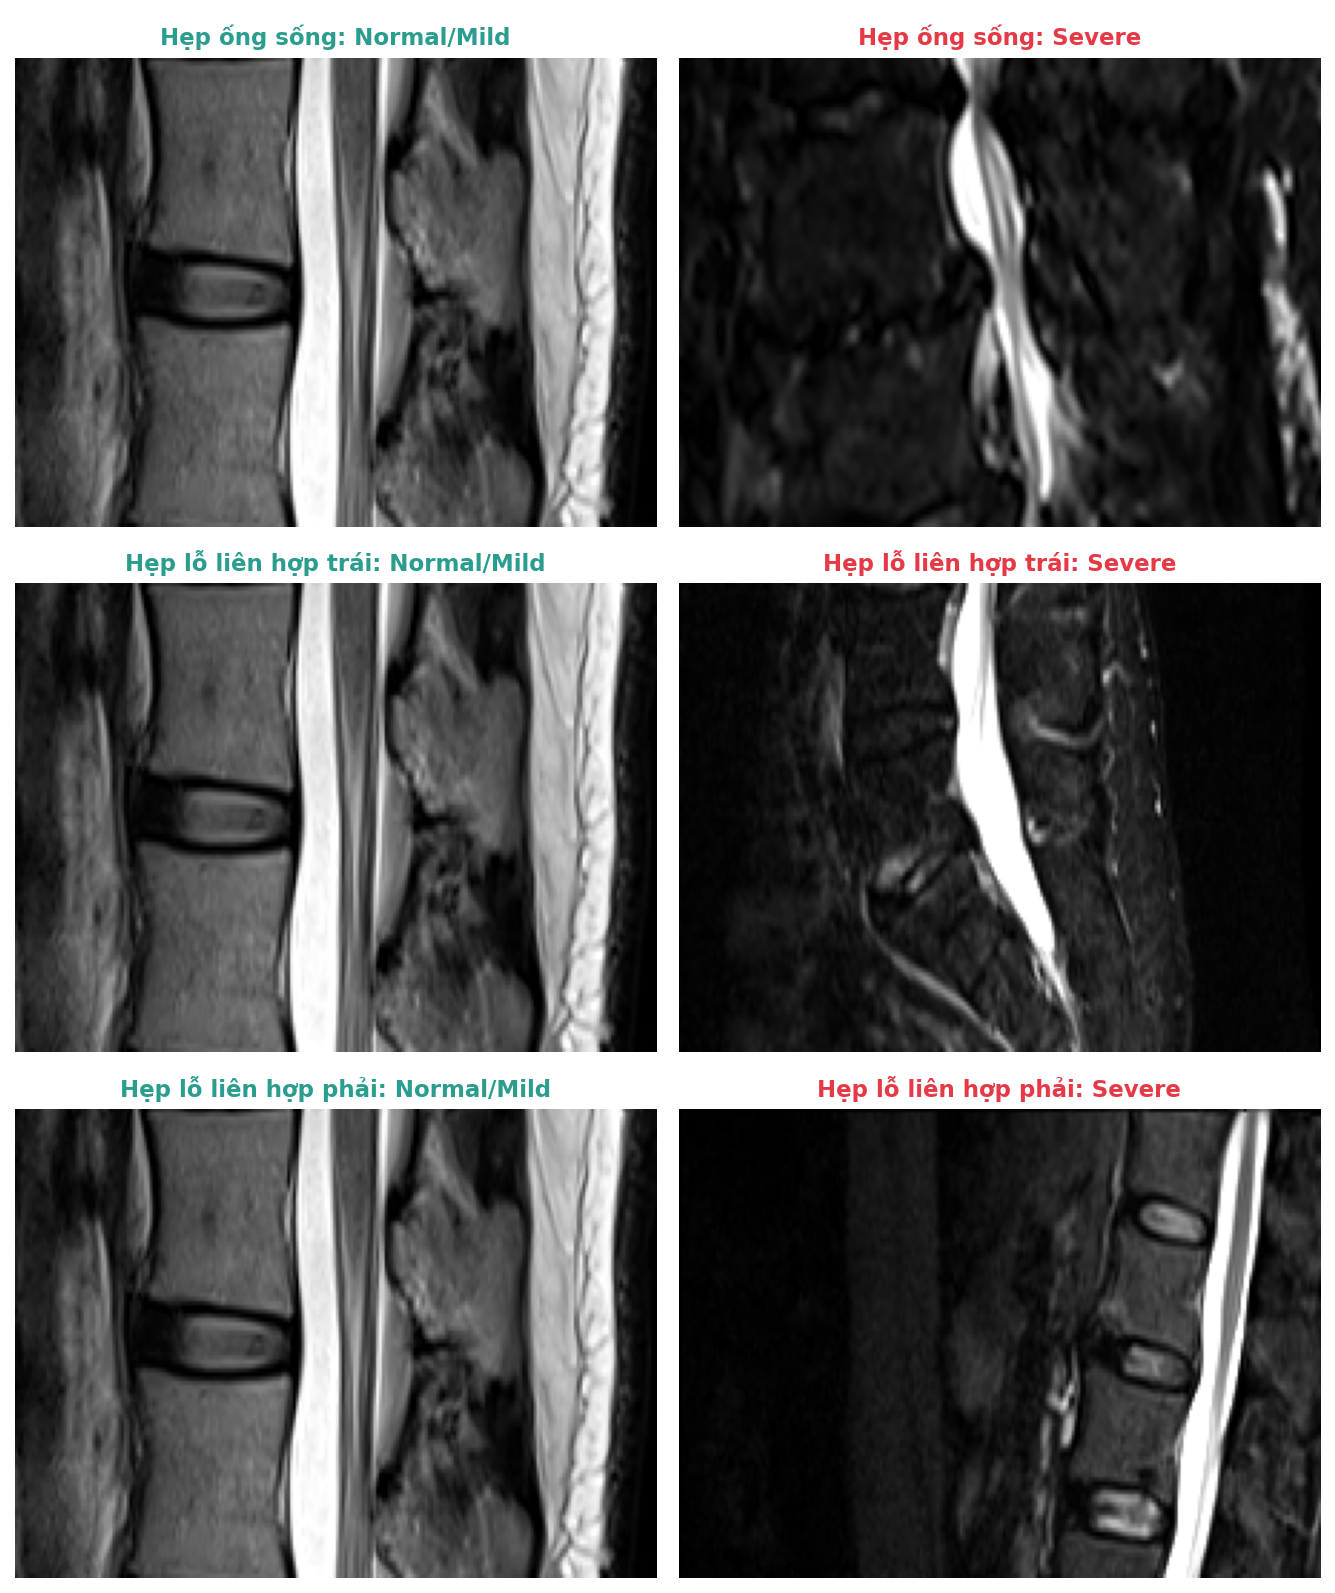
\includegraphics[width=0.85\textwidth]{cslt/abnormality_examples.png}
    \caption{Ví dụ Normal/Mild vs Severe cho 3 conditions RSNA, ảnh lấy từ bộ dữ liệu RSNA 2024~\cite{rsna2024dataset}.}
    \label{fig:abnormality_examples}
\end{figure}

% Hình~\ref{fig:spider_abnormality_examples} bổ sung minh họa cho 4 loại bất thường ở đĩa đệm và đốt sống từ SPIDER dataset, bao gồm Pfirrmann grade, thoát vị đĩa đệm, phồng đĩa đệm và trượt đốt sống.

% \begin{figure}[htbp]
%     \centering
%     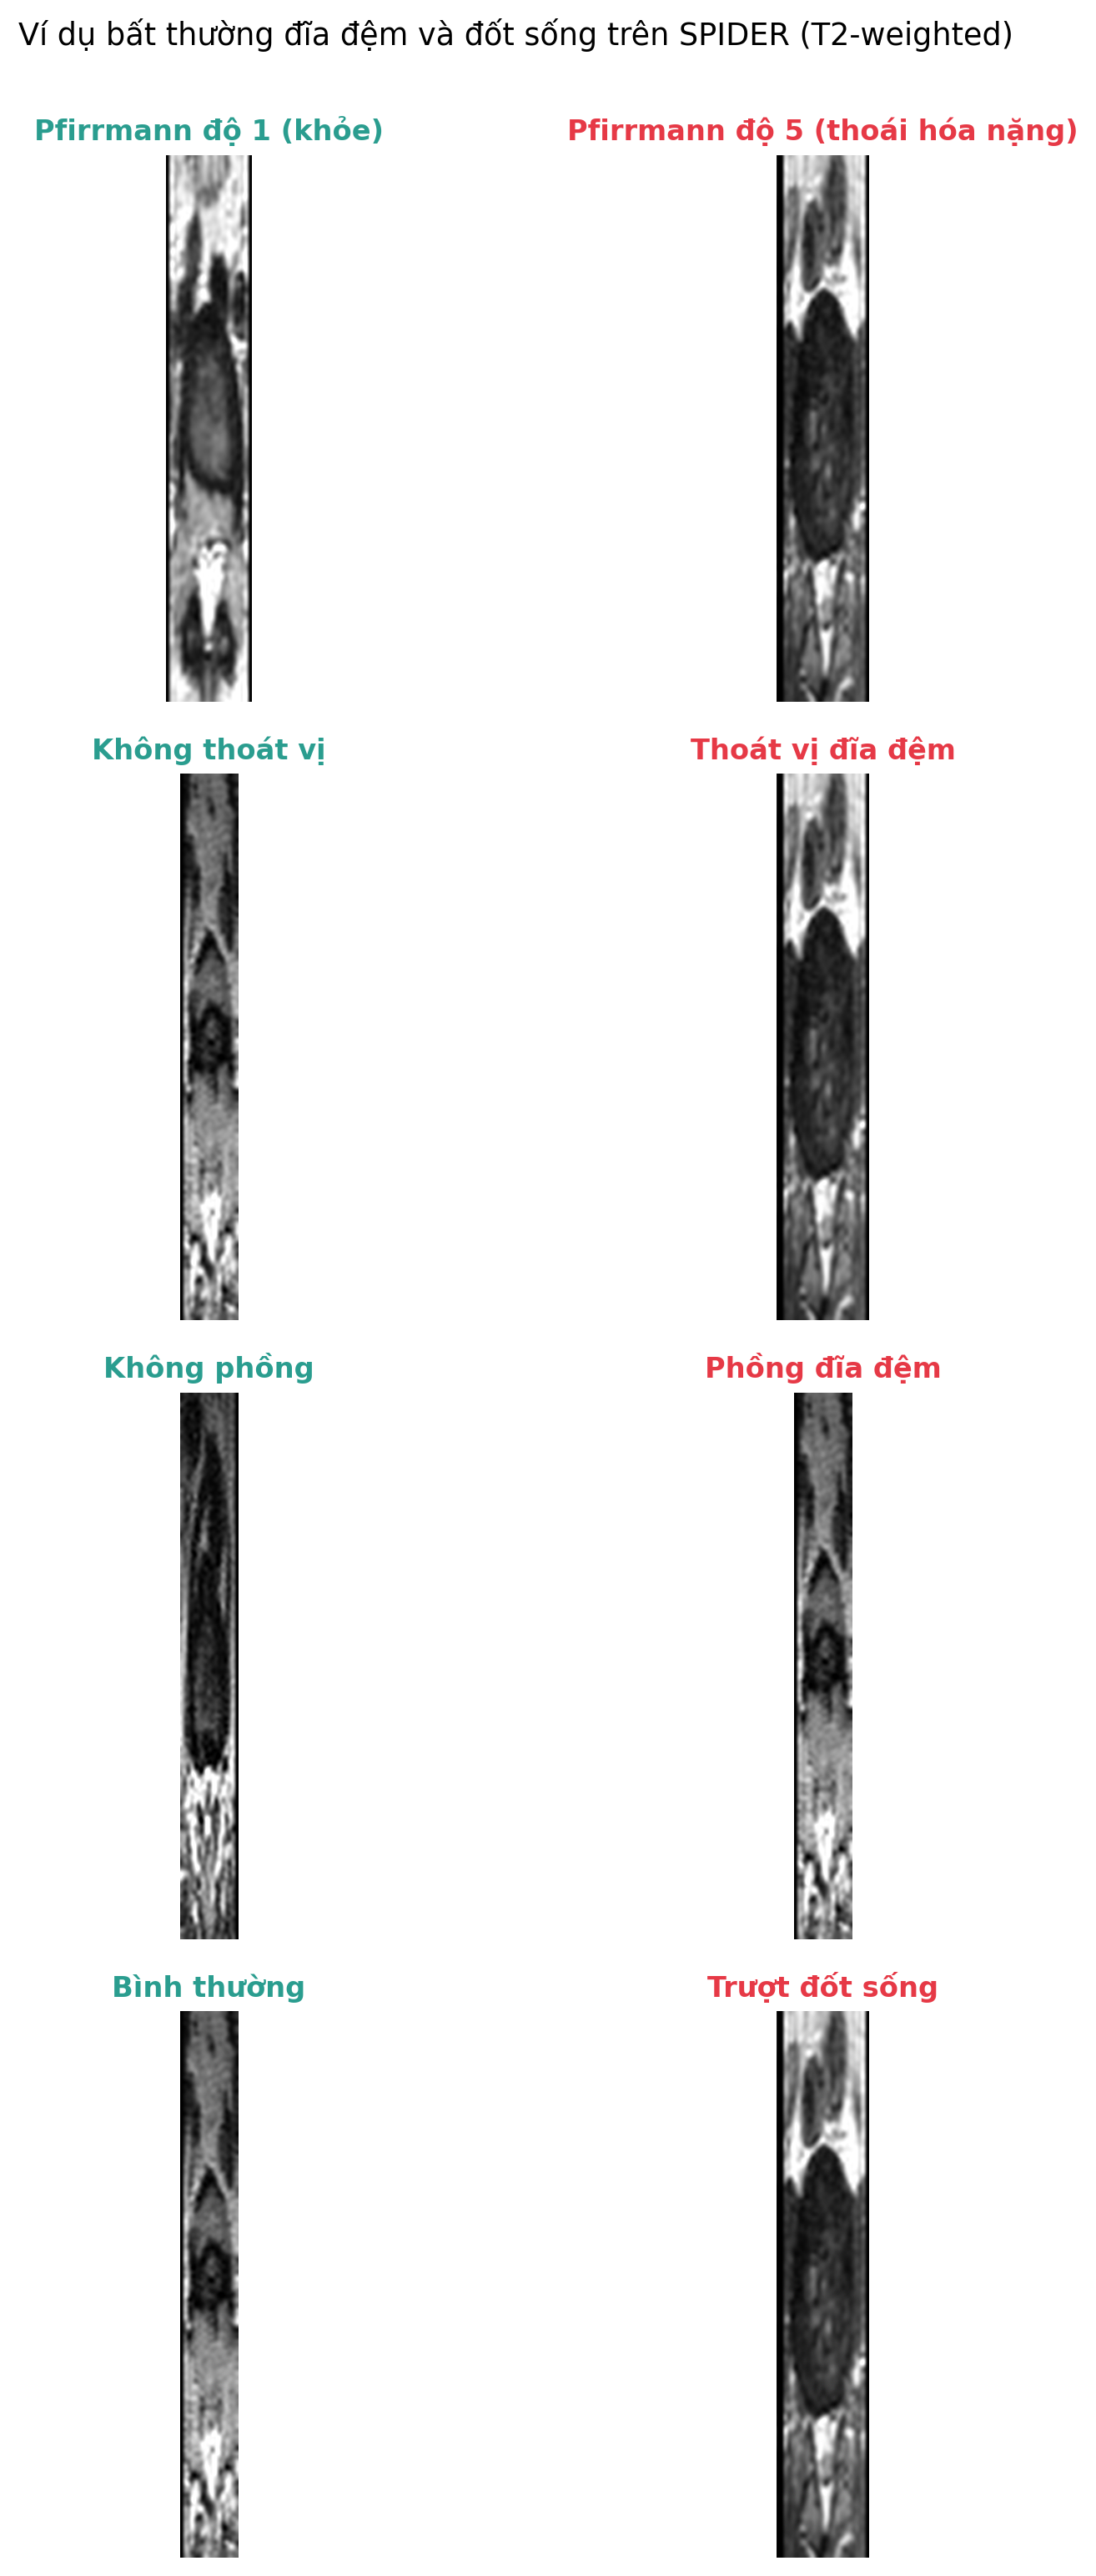
\includegraphics[width=0.75\textwidth]{cslt/spider_abnormality_examples.png}
%     \caption{Bất thường đĩa đệm và đốt sống trên SPIDER.}
%     \label{fig:spider_abnormality_examples}
% \end{figure}

\subsection{Các mặt cắt MRI và hướng chụp cơ bản}
Một khối ảnh MRI cột sống 3D có thể được trình bày dưới ba mặt cắt chính, mỗi mặt cắt phù hợp cho việc đánh giá các cấu trúc khác nhau:

\begin{itemize}
    \item \textbf{Mặt cắt dọc giữa (Sagittal):} cắt theo mặt phẳng đứng trước-sau, chia cơ thể thành hai nửa trái-phải. Đây là mặt cắt \emph{quan trọng nhất} cho việc đánh giá thoái hóa đĩa đệm, thoát vị, và sắp xếp tổng thể của cột sống. Trên ảnh Sagittal T2-weighted, đĩa đệm khỏe có tín hiệu cao (sáng), tủy sống và CSF nổi bật rõ. Luận văn sử dụng chủ yếu các lát cắt sagittal làm input cho mô hình.
    \item \textbf{Mặt cắt ngang (Axial):} cắt theo mặt phẳng ngang, vuông góc với trục cột sống. Đây là mặt cắt tốt nhất để đánh giá hẹp ống sống, hẹp ngách bên, và quan sát mối quan hệ giữa đĩa đệm với rễ thần kinh hai bên. SpineNetV2 baseline chưa khai thác mặt cắt này, đây là một hướng phát triển trong tương lai (xem Chương~\ref{chap:conclusion}).
    \item \textbf{Mặt cắt trán (Coronal):} cắt theo mặt phẳng đứng song song với lưng. Mặt cắt này ít dùng cho chẩn đoán đĩa đệm nhưng hữu ích cho việc đánh giá vẹo cột sống (scoliosis) và sắp xếp các đốt sống.
\end{itemize}

Với mỗi mặt cắt, dữ liệu MRI thường có hai chuỗi xung phổ biến:
\begin{itemize}
    \item \textbf{T1-weighted (T1):} hiển thị mô mỡ sáng, dịch tối. Dùng để đánh giá cấu trúc giải phẫu chi tiết và phát hiện biến đổi Modic type 1 (giảm tín hiệu).
    \item \textbf{T2-weighted (T2) / STIR:} hiển thị dịch sáng, mô mỡ tối hơn. Đây là chuỗi xung chính cho phát hiện viêm, phù nề, thoát vị đĩa đệm và đánh giá Pfirrmann.
\end{itemize}

\subsection{Các loại ảnh y tế thường dùng}
\textbf{X-quang (X-ray):} Là kỹ thuật cơ bản và phổ biến nhất, sử dụng tia X để tạo ra hình ảnh hai chiều của xương. X-quang rất hữu ích để đánh giá cấu trúc tổng thể của cột sống, phát hiện các vấn đề như gãy xương, trượt đốt sống, vẹo cột sống, hoặc các thay đổi thoái hóa ở xương. Tuy nhiên, X-quang có hạn chế trong việc hiển thị các mô mềm như đĩa đệm, tủy sống hay dây thần kinh.\\
    
\textbf{Cắt lớp vi tính (Computed Tomography - CT):} Kỹ thuật này cũng sử dụng tia X nhưng kết hợp với xử lý máy tính để tạo ra các hình ảnh cắt lớp ngang chi tiết của cơ thể. CT cho thấy hình ảnh xương với độ phân giải rất cao, vượt trội hơn X-quang trong việc phát hiện các gãy xương phức tạp, hẹp ống sống do xương hoặc các khối u xương. Mặc dù có thể thấy được mô mềm tốt hơn X-quang, CT vẫn không chi tiết bằng MRI.\\
    
 \textbf{Cộng hưởng từ (Magnetic Resonance Imaging - MRI):} Được xem là tiêu chuẩn vàng trong chẩn đoán các bệnh lý liên quan đến mô mềm của cột sống. MRI sử dụng từ trường mạnh và sóng radio để tạo ra hình ảnh cắt lớp chi tiết. Kỹ thuật này khảo sát xuất sắc các cấu trúc như đĩa đệm (phát hiện thoát vị), tủy sống, rễ thần kinh, dây chằng và các khối u mô mềm. MRI là công cụ không thể thiếu để chẩn đoán chính xác nguyên nhân gây chèn ép thần kinh.

\subsection{Các định dạng tệp ảnh y tế phổ biến}
Trong lĩnh vực chẩn đoán hình ảnh, dữ liệu được lưu trữ dưới nhiều định dạng khác nhau, mỗi định dạng có những đặc điểm riêng về cấu trúc và ứng dụng. Hai trong số các định dạng phổ biến nhất trong nghiên cứu và lâm sàng là DICOM và NIfTI; Bảng~\ref{tab:file_formats} tóm tắt đặc điểm của hai định dạng này.

\begin{table}[h!]
\centering
\caption{Tóm tắt đặc điểm của các định dạng tệp ảnh y tế.}
\label{tab:file_formats}
\begin{tabular}{|l|p{4cm}|l|p{5cm}|}
\hline
\textbf{Định dạng} & \textbf{Header} & \textbf{Phần mở rộng} & \textbf{Các kiểu dữ liệu} \\ \hline
NIfTI & Nhị phân, độ dài cố định (352 byte cho tệp .nii) & .nii & Số nguyên có dấu và không dấu (8-64 bit), số thực (32-128 bit), số phức (64-256 bit) \\ \hline
DICOM & Nhị phân, độ dài thay đổi & .dcm & Số nguyên có dấu và không dấu (8, 16, 32-bit). Không hỗ trợ số thực cho dữ liệu pixel. \\ \hline
\end{tabular}
\end{table}

\begin{itemize}
    \item \textbf{DICOM (Digital Imaging and Communications in Medicine):} 
    Đây không chỉ là một định dạng tệp mà còn là một tiêu chuẩn toàn diện cho việc truyền tải, lưu trữ và xử lý hình ảnh y tế. 
    \begin{itemize}
        \item[$\circ$]  \textbf{Cấu trúc:} Điểm cốt lõi và là sức mạnh lớn nhất của DICOM là dữ liệu hình ảnh (pixel) không thể tách rời khỏi siêu dữ liệu (metadata). Một tệp DICOM duy nhất chứa cả hình ảnh và một phần header cực kỳ chi tiết, bao gồm thông tin bệnh nhân, thông số kỹ thuật của máy quét, giao thức chụp (acquisition protocol),... Điều này làm cho mỗi tệp ảnh trở có đầy đủ ngữ cảnh y tế.
        \item[$\circ$]  \textbf{Header có độ dài thay đổi:} Vì phải chứa rất nhiều thông tin đa dạng, header của DICOM có độ dài thay đổi và phụ thuộc vào từng phương thức chụp (modality-dependent).
        \item[$\circ$]  \textbf{Lưu trữ dữ liệu pixel:} Dữ liệu pixel trong DICOM chỉ được lưu dưới dạng số nguyên. Để chuyển đổi sang các giá trị trong thế giới thực (ví dụ: đơn vị Hounsfield trong CT), DICOM sử dụng hai trường trong header là \texttt{slope} (độ dốc) và \texttt{intercept} (hệ số chặn) cho một phép biến đổi tuyến tính.
        \item[$\circ$]]\textbf{Ứng dụng:} Là tiêu chuẩn bắt buộc trong môi trường lâm sàng, được sử dụng bởi hầu hết các thiết bị y tế như máy MRI, CT, X-quang.
    \end{itemize}
    
    \item \textbf{NIfTI (Neuroimaging Informatics Technology Initiative):} 
    Được phát triển bởi Viện Y tế Quốc gia Hoa Kỳ (NIH), NIfTI ra đời để phục vụ riêng cho lĩnh vực nghiên cứu hình ảnh thần kinh, khắc phục một số nhược điểm của các định dạng cũ.
    \begin{itemize}
        \item[$\circ$] \textbf{Cấu trúc đơn giản:} Thông thường, dữ liệu được lưu trong một tệp duy nhất có phần mở rộng là \texttt{.nii}, gộp cả header và dữ liệu pixel. Cấu trúc này rất thuận tiện cho việc xử lý và lập trình.
        \item[$\circ$] \textbf{Header có độ dài cố định:} Không giống DICOM, header của NIfTI có kích thước cố định là 352 byte, giúp việc đọc và phân tích tệp trở nên đơn giản hơn.
        \item[$\circ$] \textbf{Thông tin không gian:} Một cải tiến quan trọng là NIfTI bổ sung thông tin về hướng (orientation) và hệ tọa độ (coordinate system) của ảnh trực tiếp vào header. Điều này giải quyết các vấn đề nhầm lẫn trái-phải thường gặp trong nghiên cứu não bộ và rất hữu ích cho các tác vụ xử lý không gian.
        \item[$\circ$] \textbf{Ứng dụng:} NIfTI là định dạng thống trị trong cộng đồng nghiên cứu khoa học, được hỗ trợ bởi hầu hết các phần mềm và thư viện phân tích hình ảnh phổ biến như FSL, SPM, Nibabel (Python).
    \end{itemize}
\end{itemize}
\subsection{Giải phẫu cột sống trên ảnh y tế}
Trên ảnh MRI hoặc CT, các cấu trúc giải phẫu của cột sống được hiển thị với các đặc điểm riêng biệt, giúp bác sĩ chẩn đoán bệnh lý. \\


\textbf{Đốt sống:} Trên cả CT và MRI, phần xương vỏ (cortical bone) của thân đốt sống có tín hiệu thấp (màu đen), trong khi phần tủy xương (bone marrow) bên trong có tín hiệu cao hơn. CT là phương tiện tốt nhất để đánh giá chi tiết cấu trúc xương. Hình~\ref{fig:lumbar_ver-abstract} minh họa hình ảnh đốt sống trên ảnh y tế.

 \begin{figure}[htbp]
        \centering
        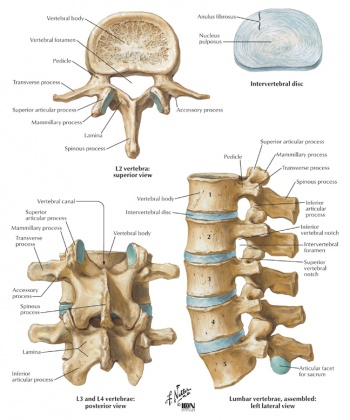
\includegraphics[scale=0.5]{cslt/lumbar_ver.jpg}
        \caption{Đốt sống~\cite{netter2003atlas}.}
        \label{fig:lumbar_ver-abstract}
    \end{figure}
\textbf{Đĩa đệm (Intervertebral Disc):} Trên ảnh MRI T2-weighted, đĩa đệm khỏe mạnh có tín hiệu cao ở trung tâm (nhân nhầy - nucleus pulposus) do chứa nhiều nước, và tín hiệu thấp hơn ở vòng ngoài (vòng sợi - annulus fibrosus). Khi đĩa đệm bị thoái hóa, nó sẽ mất nước và giảm tín hiệu (đen hơn). Thoát vị đĩa đệm là hình ảnh nhân nhầy lồi ra khỏi vị trí bình thường, có thể chèn ép vào các cấu trúc thần kinh. Hình~\ref{fig:disc-abstract} minh họa hình ảnh đĩa đệm.

 \begin{figure}[htbp]
        \centering
        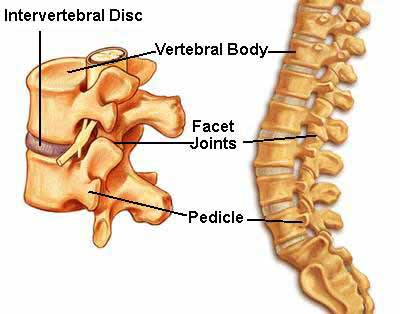
\includegraphics[scale=0.5]{cslt/disc.jpg}
        \caption{Đĩa đệm~\cite{surreyimsk_back}.}
        \label{fig:disc-abstract}
    \end{figure}

\textbf{Tủy sống và rễ thần kinh:} Các cấu trúc này được quan sát tốt nhất trên ảnh MRI. Tủy sống nằm trong ống sống, được bao quanh bởi dịch não tủy (cerebrospinal fluid - CSF) có tín hiệu rất cao (màu trắng) trên ảnh T2-weighted. Các rễ thần kinh từ tủy sống đi ra qua các lỗ liên hợp, và sự chèn ép lên chúng bởi đĩa đệm hoặc xương là nguyên nhân phổ biến gây đau thần kinh tọa. Hình~\ref{fig:spinal-cord-abstract} minh họa tủy sống và rễ thần kinh.
\begin{figure}[htbp]
        \centering
        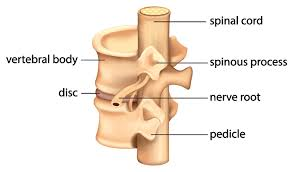
\includegraphics[scale=0.8]{cslt/spinal_cord.jpg}
        \caption{Tủy sống và rễ thần kinh~\cite{sspine_spine}.}
        \label{fig:spinal-cord-abstract}
\end{figure}

\section{Mô hình Artificial Neural Network - ANN}
Mô hình Artificial Neural Network - ANN (Mạng nơ-ron nhân tạo) \cite{NN}
là mô hình tính toán được xây dựng lấy ý tưởng từ cấu trúc và cách
hoạt động của mạng nơ-ron thần kinh trong não người nhằm thực hiện một
tác vụ nào đó với tập thông tin đầu vào. Một mạng nơ-ron thần kinh được tạo nên từ nhiều nơ-ron sinh học kết
nối và hoạt động cùng nhau. Chúng hoạt động bằng cách tiếp nhận các thông tin đưa vào
từ các \textit{đuôi gai} (dendrite), tính toán và tổng hợp tại \textit{thân nơ-ron} (cell body),
sau đó lan truyền kết quả đến các nơ-ron khác thông qua \textit{sợi trục} (axon). Có thể dễ dàng rút ra nhận xét rằng \textbf{nơ-ron sinh học nhận nhiều thông
tin đầu vào nhưng chỉ đưa ra một kết quả duy nhất thôngc qua quá trình xử lý trung gian phức tạp}.

Tương tự như cách thức hoạt động nêu trên của mạng nơ-ron thần kinh,
ANN cũng được cấu thành từ nhiều nơ-ron được gọi là perceptron có cấu
trúc như Hình~\ref{fig:perceptron}. Trong đó:

\begin{itemize}
    \item[--] $x_1, x_2, x_3, ..., x_n$ lần lượt là các biến đại diện cho dữ liệu đầu vào.

    \item[--] phép cộng (\textit{summation}) và hàm kích hoạt (\textit{activation function})
là các phép tính toán và tổng hợp các thông tin dữ liệu đầu vào.

    \item[--] $w_1, w_2, w_3, ..., w_n$ là các trọng số cần phải học, đóng vai trò tham
gia quá trình tính toán và chuyển đổi các thông tin đầu vào thành
thông tin đầu ra.

    \item[--] $\hat{y}$ là output của tiến trình, đại diện cho dữ liệu đầu ra.

\end{itemize}

\begin{figure}[!htb]
        \centering
        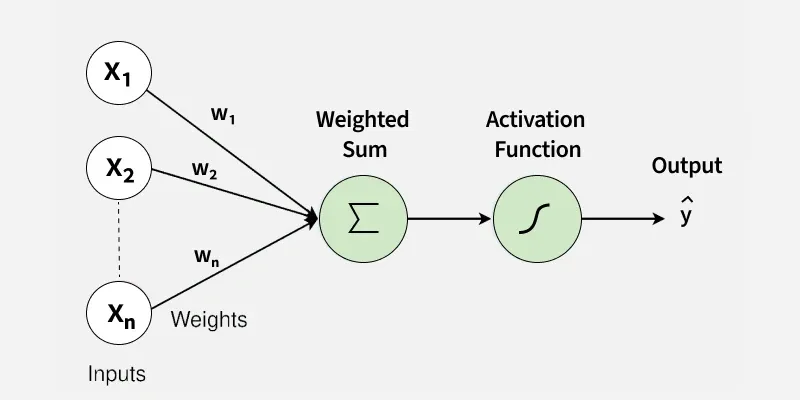
\includegraphics[width=0.75\textwidth]{cslt/perceptron.png}
        \caption{Cấu trúc của một Perceptron~\cite{gfg_perceptron}.}
        \label{fig:perceptron}
    \end{figure}

Cụ thể hơn, phương thức tính toán và tổng hợp dữ liệu của một perceptron được mô tả theo từng bước sau:

\begin{enumerate}
    \item Perceptron
thực hiện phép cộng bằng cách tính tổng giá trị tất cả các tích số của
từng cặp dữ liệu đầu vào và giá trị trọng số tương ứng:

\begin{equation}
    a = \sum_{i = 1}^n w_ix_i + w_0
\end{equation}

    \item Kết quả $a$ của phép cộng được đưa qua một hàm kích hoạt phi
tuyến như \textit{Sigmoid, Tanh, ReLU, LeakyReLU} được minh họa ở Hình~\ref{fig:act_functions}.


\begin{figure}[!htb]
        \centering
        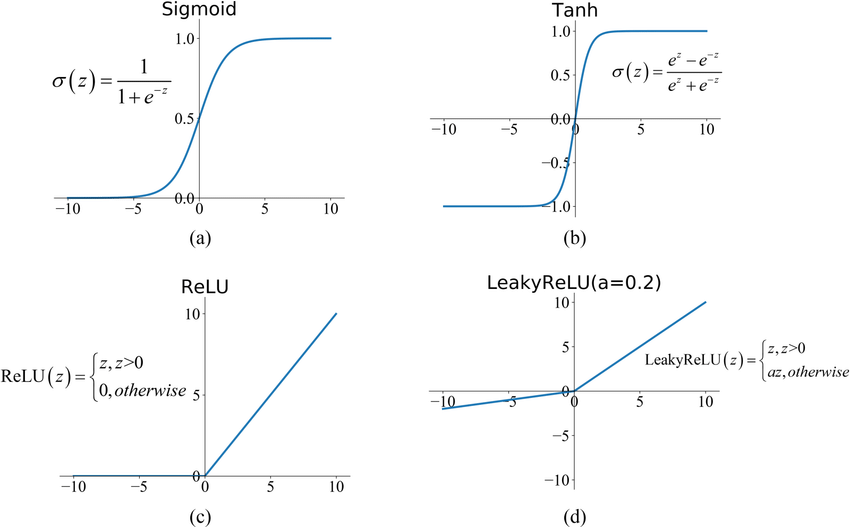
\includegraphics[width=0.85\textwidth]{cslt/act.png}
        \caption{Các hàm phi tuyến được sử dụng trong Perceptron \cite{goodfellow2016deep}.}
        \label{fig:act_functions}
    \end{figure}

    \item Sau đó, perceptron thực hiện phép so sánh giá trị nhận được từ hàm
kích hoạt \textit{f(a)} với một giá trị ngưỡng (\textit{threshold}) cho trước nhằm
xác định giá trị đầu ra $\hat{y}$ như là tín hiệu kích hoạt của perceptron.

\begin{equation}
    \hat{y} = \left\{\begin{matrix}
1   & \text{if} f(a) \geq \text{threshold}\\ 
0 &  \text{if} f(a) < \text{threshold}
\end{matrix}\right.
\end{equation}
\end{enumerate}

Bằng cách kết hợp nhiều perceptron với nhau sẽ tạo nên cấu trúc mô
hình mạng ANN. Mạng ANN bao gồm nhiều perceptron như là các nút mạng tính toán làm tăng tính phức tạp cũng như khả năng học cho mạng, các perceptron đó hình thành nên các tầng như sau:

\begin{itemize}
    \item[--] \textbf{Tầng đầu vào} (input layer): là tầng đầu tiên, thể hiện các dữ liệu đầu
vào của mô hình.
    \item[--] \textbf{Tầng ẩn} (hidden layer): là tầng nằm giữa gồm các phép tính toán nhằm
chuyển đổi dữ liệu đầu vào sang dữ liệu đầu ra. 

    \item[--] \textbf{Tầng kết quả} (output layer): là tầng cuối cùng thể hiện dữ liệu đầu ra của mạng. 
\end{itemize}

Số lượng tầng ẩn trong mô hình ANN là không giới hạn và được xác
định tùy thuộc vào bài toán cần giải quyết. Đặc biệt, khi số lượng tầng ẩn
lớn hơn 1 thì mô hình ANN được gọi là mô hình \textit{Học sâu} (Deep learning).

\section{ Mạng tích chập Convolutional Neural Network - CNN }
Mạng tích chập có 02 phần chính: \textbf{Lớp trích lọc đặc trưng của ảnh} (Conv, Relu và Pool) và \textbf{Lớp phân loại} (FC và softmax). Hình~\ref{fig:cnn} minh họa cấu trúc tổng thể của một mạng CNN cơ bản.\\
\begin{figure}[!htb]
        \centering
        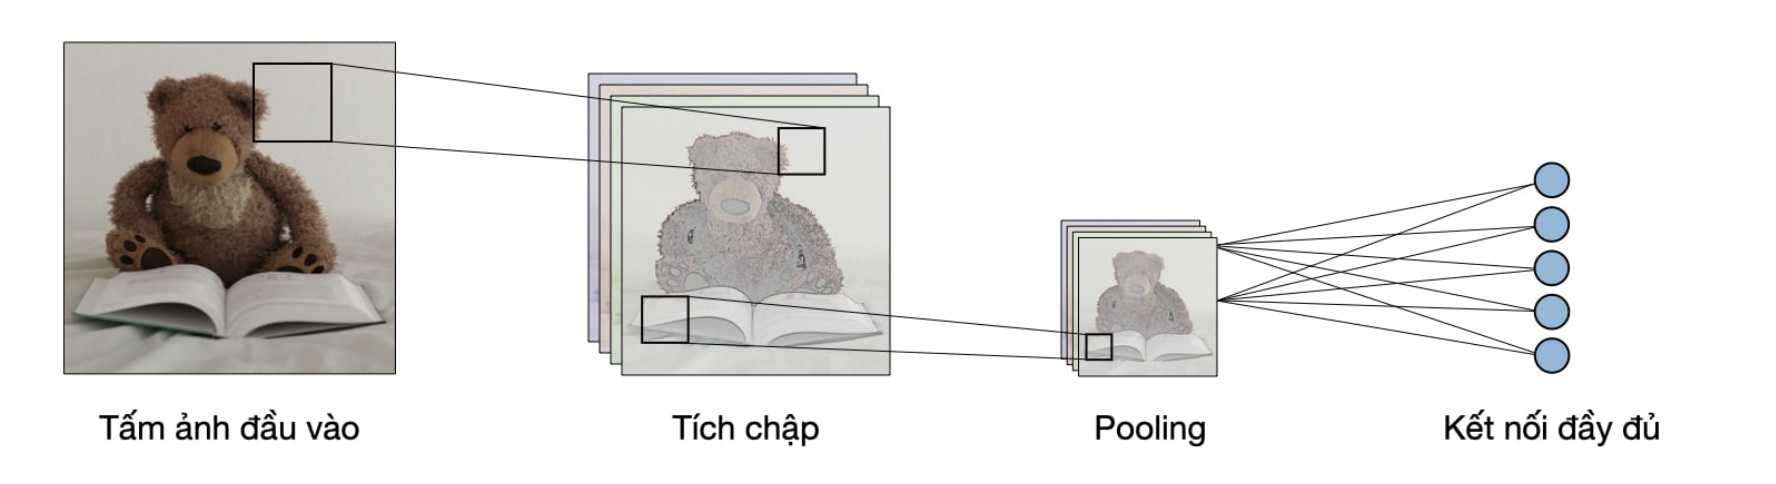
\includegraphics[width=\textwidth]{cslt/cnn.png}
        \caption{Mô hình CNN cơ bản \cite{shegaonkar2024cnn}.}
        \label{fig:cnn}
\end{figure}
Đầu vào (dữ liệu training):
\begin{itemize}
    \item Input đầu vào là một bức ảnh được biểu diển bởi ma trận pixel với kích thước: $[w \times h \times d]$
    \item W: chiều rộng
\item  H: chiều cao
\item  D: Là độ sâu, hay dễ hiểu là số lớp màu của ảnh. Ví dụ ảnh RBG sẽ là 3 lớp ảnh Đỏ, Xanh Dương, Xanh.
\end{itemize}

\textbf{Conv layer:} Mục tiêu của các lớp tích chập là trích chọn các đặc trưng của ảnh đầu vào. Ảnh đầu vào được cho qua một bộ lọc chạy dọc bức ảnh. Bộ lọc có kích thước là $m \times n$ và áp dụng phép tích vô hướng để tính toán, cho ra một giá trị duy nhất. Đầu ra của phép tích chập là một tập các giá trị ảnh được gọi là mạng đặc trưng (features map).\\

Phép tích chập đơn giản là phép tìm biên ảnh. Sau khi cho qua bộ lọc nó sẽ làm hiện lên các đặc trưng của đối tượng trong ảnh như đường vẽ xung quanh đối tượng, các góc cạnh,v.v.., và các layer tiếp theo sẽ lại trích xuất tiếp các đặc trưng của đặc trưng của các đối tượng đó, việc có nhiều layer như vậy cho phép chúng ta chia nhỏ đặc trưng của ảnh tới mức nhỏ nhất có thể.\\

\textbf{ReLU layer:} ReLU layer áp dụng các kích hoạt (activation function) max(0,x) lên đầu ra của Conv Layer, có tác dụng đưa các giá trị âm về thành 0. Layer này không thay đổi kích thước của ảnh và không có thêm bất kì tham số nào. Mục đích của lớp ReLu là đưa ảnh một mức ngưỡng, ở đây là 0. Để loại bỏ các giá trị âm không cần thiết mà có thể sẽ ảnh hưởng cho việc tính toán ở các layer sau đó.\\

\textbf{Pool layer:} Pool Layer thực hiện chức năng làm giảm chiều không gian của đầu và giảm độ phức tạp tính toán của model ngoài ra Pool Layer còn giúp kiểm soát hiện tượng overffiting. Thông thường, Pool layer có nhiều hình thức khác nhau phù hợp cho nhiều bài toán, tuy nhiên Max Pooling là được sử dụng nhiều vào phổ biến hơn cả với ý tưởng cũng rất sát với thực tế con người đó là: Giữ lại chi tiết quan trọng hay hiểu ở trong bài toán này chính giữ lại pixel có giá trị lớn nhất.\\

\textbf{Fully connected layer (FC):} Tên tiếng việt là Mạng liên kết đầy đủ. Tại lớp mạng này, mỗi một nơ-ron của layer này sẽ liên kết tới mọi nơ-ron của lớp khác. Để đưa ảnh từ các layer trước vào mạng này, buộc phải dàn phẳng bức ảnh ra thành 1 vector thay vì là mảng nhiều chiều như trước. Tại layer cuối cùng sẽ sử dụng 1 hàm kinh điển trong học máy softmax để phân loại đối tượng dựa vào vector đặc trưng đã được tính toán của các lớp trước đó.
\section{Kiến trúc Encoder-Decoder}
Kiến trúc Encoder-Decoder là một mô hình mạng nơ-ron được thiết kế để giải quyết các bài toán \textbf{chuỗi-đến-chuỗi (sequence-to-sequence - Seq2Seq)}, nơi độ dài của chuỗi đầu vào và chuỗi đầu ra có thể khác nhau. Mô hình này đã trở thành nền tảng cho nhiều ứng dụng đột phá trong xử lý ngôn ngữ tự nhiên như dịch máy, tóm tắt văn bản, và trả lời câu hỏi \cite{sutskever2014seq2seq, cho2014learning}. Hình~\ref{fig:en-de-abstract} minh họa kiến trúc Encoder-Decoder tổng quát.

\begin{figure}[H]
        \centering
        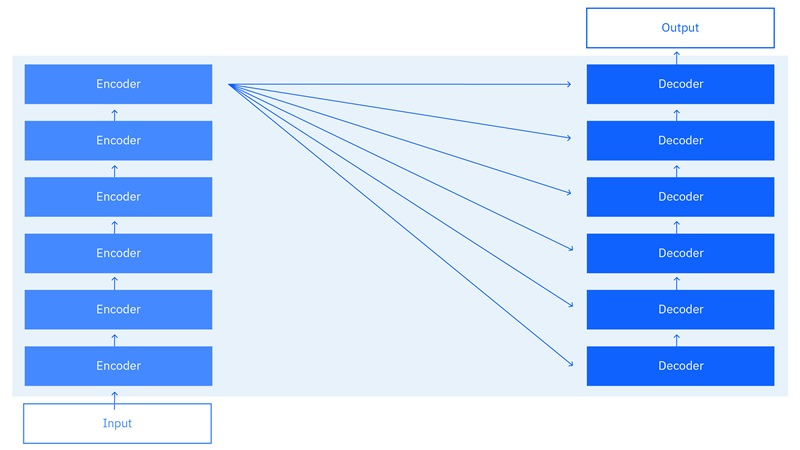
\includegraphics[width=\textwidth]{cslt/en-de.png}
        \caption{Kiến trúc Encoder-Decoder \cite{ibm_encoderdecoder}.}
        \label{fig:en-de-abstract}
\end{figure}

Về cơ bản, kiến trúc này bao gồm hai thành phần chính: \textbf{Encoder (Bộ mã hóa)} và \textbf{Decoder (Bộ giải mã)}, thường được xây dựng từ các mạng nơ-ron hồi quy (RNN), đặc biệt là LSTM (Long Short-Term Memory) hoặc GRU (Gated Recurrent Unit).



\subsection{Encoder}
Nhiệm vụ của Encoder là đọc và "hiểu" chuỗi đầu vào, sau đó nén toàn bộ thông tin của chuỗi đó thành một vector có kích thước cố định, được gọi là \textbf{vector ngữ cảnh (context vector)} hoặc "vector tư tưởng" (thought vector).

Quá trình này diễn ra tuần tự qua từng phần tử của chuỗi đầu vào.
\begin{itemize}
    \item Cho một chuỗi đầu vào $X = (x_1, x_2, \dots, x_T)$, tại mỗi bước thời gian $t$, mạng RNN của Encoder sẽ cập nhật trạng thái ẩn (hidden state) $h_t$ dựa trên phần tử đầu vào $x_t$ và trạng thái ẩn của bước trước đó $h_{t-1}$.
    \item Công thức cập nhật trạng thái ẩn có thể được biểu diễn tổng quát như sau:
    \begin{equation}
        h_t = f(W_{hh}h_{t-1} + W_{xh}x_t)
    \end{equation}
    Trong đó, $f$ là một hàm phi tuyến tính (ví dụ như hàm kích hoạt của LSTM hoặc GRU), $W_{hh}$ và $W_{xh}$ là các ma trận trọng số được huấn luyện.
    \item Sau khi xử lý toàn bộ chuỗi đầu vào qua $T$ bước, trạng thái ẩn cuối cùng $h_T$ chính là vector ngữ cảnh $C$. Vector này được kỳ vọng sẽ chứa đựng tóm tắt toàn bộ ý nghĩa của chuỗi đầu vào.
    \begin{equation}
        C = h_T
    \end{equation}
\end{itemize}

\subsection{Decoder}
Nhiệm vụ của Decoder là nhận vector ngữ cảnh $C$ từ Encoder và tạo ra chuỗi đầu ra $Y = (y_1, y_2, \dots, y_{T'})$.

\begin{itemize}
    \item Decoder cũng là một mạng RNN. Trạng thái ẩn ban đầu của nó, $s_0$, được khởi tạo bằng chính vector ngữ cảnh $C$ từ Encoder.
    \begin{equation}
        s_0 = C
    \end{equation}
    \item Tại mỗi bước thời gian $t$, Decoder sẽ tạo ra một phần tử $y_t$ của chuỗi đầu ra. Quá trình này có tính tự hồi quy (auto-regressive), nghĩa là đầu ra của bước trước $y_{t-1}$ sẽ được dùng làm đầu vào cho bước hiện tại $t$.
    \item Trạng thái ẩn $s_t$ của Decoder được cập nhật như sau:
    \begin{equation}
        s_t = g(W_{ss}s_{t-1} + W_{ys}y_{t-1})
    \end{equation}
    Trong đó, $g$ là hàm kích hoạt của RNN trong Decoder, $W_{ss}$ và $W_{ys}$ là các ma trận trọng số.
    \item Từ trạng thái ẩn $s_t$, mô hình sẽ dự đoán xác suất của từ tiếp theo trong chuỗi đầu ra thông qua một lớp softmax trên toàn bộ bộ từ vựng:
    \begin{equation}
        P(y_t | y_1, \dots, y_{t-1}, C) = \text{softmax}(W_{sy}s_t)
    \end{equation}
\end{itemize}

\subsection{Cơ chế tập trung}
Kiến trúc Encoder-Decoder cơ bản có một hạn chế lớn: nó phải nén toàn bộ thông tin của chuỗi đầu vào vào một vector ngữ cảnh $C$ có kích thước cố định. Đây trở thành một \textbf{"nút thắt cổ chai" (bottleneck)} thông tin, đặc biệt với các chuỗi đầu vào dài, khiến mô hình khó có thể ghi nhớ các chi tiết ở phần đầu của chuỗi.

Để giải quyết vấn đề này, \textbf{cơ chế Tập trung (Attention Mechanism)} đã được giới thiệu. Thay vì chỉ sử dụng trạng thái ẩn cuối cùng của Encoder, cơ chế attention cho phép Decoder tại mỗi bước giải mã có thể "nhìn lại" và tập trung vào tất cả các trạng thái ẩn của Encoder ($h_1, h_2, \dots, h_T$).
\begin{itemize}
    \item Tại mỗi bước tạo ra đầu ra $y_i$, Decoder sẽ tính toán một bộ "trọng số tập trung" $\alpha_{ij}$ cho mỗi trạng thái ẩn $h_j$ của Encoder. Trọng số này cho biết mức độ quan trọng của từ đầu vào thứ $j$ đối với việc tạo ra từ đầu ra thứ $i$.
    \item Một vector ngữ cảnh động $c_i$ được tính bằng tổng có trọng số của tất cả các trạng thái ẩn của Encoder:
    \begin{equation}
        c_i = \sum_{j=1}^{T} \alpha_{ij} h_j
    \end{equation}
    \item Vector ngữ cảnh động $c_i$ này sau đó được sử dụng để dự đoán đầu ra $y_i$. Bằng cách này, mô hình có thể tập trung vào các phần phù hợp của chuỗi đầu vào khi tạo ra từng phần của chuỗi đầu ra, giúp cải thiện đáng kể hiệu suất, đặc biệt là với các chuỗi dài.
\end{itemize}

\section{Kiến trúc U-Net}
U-Net là một kiến trúc mạng nơ-ron tích chập (CNN) được thiết kế đặc biệt cho bài toán \textbf{phân vùng ảnh y tế (biomedical image segmentation)}, được giới thiệu lần đầu bởi Ronneberger và cộng sự 
\cite{ronneberger2015unet}. Tên gọi "U-Net" xuất phát từ hình dạng chữ U đặc trưng của kiến trúc này (Hình~\ref{fig:unet}). Về bản chất, U-Net là một mô hình \textbf{Encoder-Decoder} được cải tiến, bao gồm hai phần chính: một \textbf{đường đi xuống (contracting path)} để nắm bắt ngữ cảnh và một \textbf{đường đi lên (expansive path)} để tái tạo ảnh và định vị chính xác.

\begin{figure}[!htb]
        \centering
        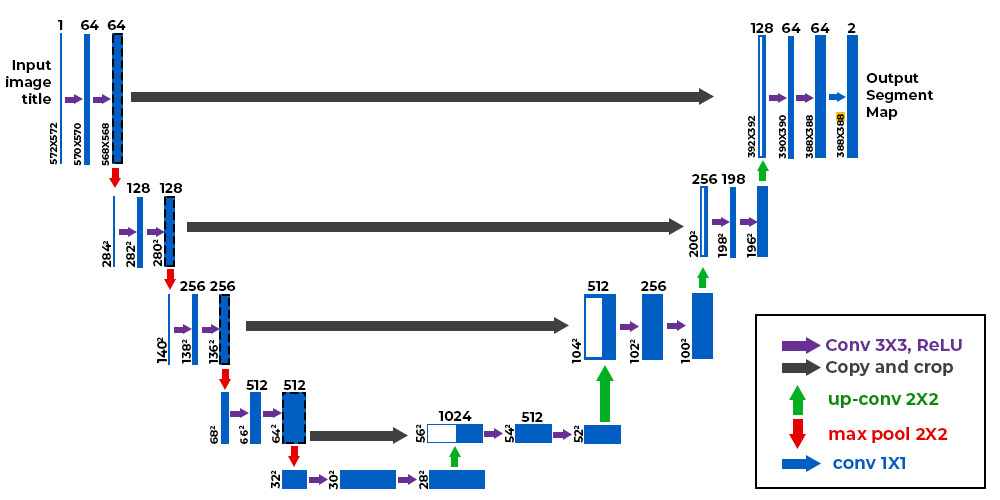
\includegraphics[width=\textwidth]{cslt/unet-arch.jpeg}
        \caption{Kiến trúc U-Net~\cite{ronneberger2015unet, gfg_unet}.}
        \label{fig:unet}
\end{figure}

Phần đầu tiên, \textbf{đường đi xuống (Encoder)}, hoạt động như một bộ trích xuất đặc trưng. Nó bao gồm các khối lặp lại, mỗi khối chứa hai lớp tích chập 3x3 (theo sau là hàm kích hoạt ReLU) và một lớp gộp cực đại 2x2 (max pooling). Quá trình này giúp giảm dần kích thước không gian của ảnh (downsampling) trong khi tăng dần số lượng kênh đặc trưng. Nhờ đó, mô hình có thể học được các thông tin ngữ cảnh phức tạp và trừu tượng của ảnh đầu vào, hay nói cách khác là "hiểu được cái gì" đang có trong ảnh, nhưng lại làm mất đi thông tin về vị trí chính xác.

Đối xứng với nó là \textbf{đường đi lên (Decoder)}. Nhiệm vụ của phần này là xây dựng lại một bản đồ phân vùng có độ phân giải cao từ các đặc trưng đã được mã hóa. Tại mỗi bước, nó sử dụng một lớp tích chập chuyển vị 2x2 (transposed convolution) để tăng kích thước không gian lên gấp đôi (upsampling). Điểm cải tiến cốt lõi và làm nên sức mạnh của U-Net chính là các \textbf{kết nối tắt (skip connections)}. Tại mỗi bước đi lên, bản đồ đặc trưng sau khi được tăng kích thước sẽ được ghép (concatenate) với bản đồ đặc trưng có cùng độ phân giải từ đường đi xuống tương ứng. Các kết nối tắt này cho phép mô hình kết hợp thông tin ngữ cảnh trừu tượng từ Decoder với thông tin không gian chi tiết, có độ phân giải cao từ Encoder. Sự kết hợp này giúp giải quyết vấn đề mất mát thông tin vị trí, cho phép mô hình định vị các đối tượng một cách cực kỳ chính xác – tức là "biết được nó nằm ở đâu". Sau khi ghép, khối này tiếp tục được xử lý qua hai lớp tích chập 3x3.

Cuối cùng, một lớp tích chập 1x1 được sử dụng ở lớp cuối cùng để ánh xạ bản đồ đặc trưng đa kênh thành bản đồ phân vùng cuối cùng với số kênh tương ứng với số lớp đối tượng cần phân loại.
\section{Context-Aware Transformers}
Trong khi các mạng CNN (như U-Net) rất mạnh trong việc trích xuất các đặc trưng cục bộ chi tiết, chúng lại gặp khó khăn trong việc nắm bắt các mối quan hệ ngữ cảnh ở phạm vi xa  trong một tấm ảnh. Ngược lại, kiến trúc Transformer, vốn thành công trong xử lý ngôn ngữ, lại có khả năng mô hình hóa các mối quan hệ toàn cục nhưng có thể bỏ qua các chi tiết kết cấu ở mức độ pixel.

Để kết hợp ưu điểm của cả hai phương pháp, kiến trúc \textbf{Context-Aware Transformers} đã được đề xuất, đặc biệt cho các bài toán phân vùng y tế, nơi cả ngữ cảnh toàn cục và chi tiết cục bộ đều cực kỳ quan trọng \cite{windsor2022context}. Ý tưởng cốt lõi là tạo ra một mô hình "nhận thức được ngữ cảnh" bằng cách kết hợp song song hai luồng xử lý thông tin.

Kiến trúc này thường bao gồm một bộ mã hóa \textbf{hai nhánh}:
\begin{enumerate}
    \item \textbf{Nhánh nhận thức cục bộ (Local-Aware Branch):} Thường là một mạng CNN (ví dụ: một phần của kiến trúc ResNet). Nhánh này có nhiệm vụ xử lý ảnh đầu vào và trích xuất các bản đồ đặc trưng (feature maps) giàu thông tin về kết cấu, hình dạng và các chi tiết ở phạm vi hẹp. Đây là thế mạnh truyền thống của CNN.

    \item \textbf{Nhánh nhận thức toàn cục (Global-Aware Branch):} Đây là một kiến trúc dựa trên Transformer (cụ thể là Vision Transformer - ViT). Ảnh đầu vào được chia thành các "mảnh" (patches) nhỏ, sau đó được "dát phẳng" và đưa vào các khối Transformer Encoder. Nhờ cơ chế tự tập trung (self-attention), nhánh này có thể học được mối tương quan giữa tất cả các cặp mảnh ảnh, bất kể chúng nằm ở đâu. Điều này cho phép mô hình nắm bắt được ngữ cảnh tổng thể của bức ảnh.
\end{enumerate}

Điểm mấu chốt của mô hình là một \textbf{mô-đun hợp nhất (fusion module)} được thiết kế để kết hợp hiệu quả thông tin từ hai nhánh trên. Các đặc trưng cục bộ chi tiết từ nhánh CNN sẽ được làm giàu thêm bằng các thông tin ngữ cảnh toàn cục từ nhánh Transformer. Biểu diễn kết hợp này sau đó được đưa vào một bộ giải mã, thường có cấu trúc tương tự như U-Net, để tái tạo lại bản đồ phân vùng cuối cùng.

Bằng cách này, Context-Aware Transformer có thể vừa tận dụng khả năng nắm bắt chi tiết tinh vi của CNN, vừa khai thác được khả năng hiểu ngữ cảnh toàn cục của Transformer, từ đó cải thiện đáng kể độ chính xác trong các tác vụ phân vùng phức tạp.

\section{Cơ chế attention CBAM (Convolutional block attention module)}
\label{sec:cbam_theory}
Mặc dù mạng tích chập (CNN) trích xuất đặc trưng tốt từ ảnh, không phải mọi kênh đặc trưng và mọi vị trí không gian đều mang thông tin hữu ích như nhau cho bài toán phân loại. Đặc biệt với ảnh y tế, vùng bệnh lý (ví dụ vùng thoát vị đĩa đệm, vùng hẹp ống sống) thường chiếm tỉ lệ rất nhỏ so với toàn bộ khối ảnh đầu vào. \textbf{CBAM (Convolutional Block Attention Module)} được Woo và cộng sự \cite{woo2018cbam} giới thiệu năm 2018 là một mô-đun chú ý nhẹ, có thể chèn vào bất kì vị trí nào của một CNN, giúp mô hình tự động học cách "tập trung" vào các kênh đặc trưng và các vị trí không gian quan trọng nhất.

CBAM bao gồm hai phần tuần tự: \textbf{chú ý theo kênh} (Channel Attention) và \textbf{chú ý theo không gian} (Spatial Attention). Với đầu vào là một tensor đặc trưng $F$ có kích thước $C \times H \times W$, phần Channel Attention tính một vector chú ý theo kênh $M_c$ kích thước $C \times 1 \times 1$ qua các bước:
\begin{itemize}
    \item Áp dụng đồng thời Average Pooling và Max Pooling trên chiều không gian, thu được hai vector kích thước $C \times 1 \times 1$.
    \item Đưa hai vector này qua cùng một mạng MLP hai lớp (chia sẻ trọng số) để học các quan hệ phi tuyến giữa các kênh.
    \item Cộng hai đầu ra và đưa qua hàm sigmoid để chuẩn hóa về khoảng $[0, 1]$.
\end{itemize}

Công thức được viết tóm tắt như sau:
\begin{equation}
M_c(F) = \sigma\left(\text{MLP}(\text{AvgPool}(F)) + \text{MLP}(\text{MaxPool}(F))\right)
\end{equation}

Vector $M_c$ sau đó được nhân theo từng kênh với $F$ ban đầu để khuếch đại các kênh quan trọng và làm yếu các kênh ít liên quan: $F' = M_c(F) \otimes F$.

Phần Spatial Attention nhận đầu ra $F'$ từ bước trên và sinh một mặt nạ chú ý theo không gian $M_s$ kích thước $1 \times H \times W$:
\begin{itemize}
    \item Áp dụng Average Pooling và Max Pooling theo chiều kênh, thu được hai feature map kích thước $1 \times H \times W$.
    \item Ghép hai feature map này theo chiều kênh thành tensor kích thước $2 \times H \times W$.
    \item Đưa qua một lớp convolution $7 \times 7$ (filter size lớn để bắt được ngữ cảnh không gian rộng), sau đó qua hàm sigmoid.
\end{itemize}

Công thức:
\begin{equation}
M_s(F') = \sigma\left(\text{Conv}_{7\times 7}\left([\text{AvgPool}(F'); \text{MaxPool}(F')]\right)\right)
\end{equation}

Đầu ra cuối cùng là $F'' = M_s(F') \otimes F'$.

CBAM rất phù hợp cho bài toán ảnh y tế vì hai lý do chính. Thứ nhất, số tham số mà CBAM thêm vào rất ít, chỉ vài chục nghìn so với hàng chục triệu của backbone CNN, nên không gây overfitting trên các dataset y tế thường có quy mô nhỏ. Thứ hai, cơ chế chú ý ngầm cho phép mô hình học cách "nhìn vào đâu" mà không cần thông tin định vị thủ công (ví dụ bounding box hay mặt nạ phân vùng). Trong luận văn này, CBAM được chèn sau mỗi stage của 3D ResNet-34 (4 stages tương ứng 64, 128, 256, 512 kênh) trong nhánh trainable của kiến trúc Hybrid đề xuất ở Chương 4.


\section{Các mô hình nền tảng trong ảnh y tế}

\subsection{Mô hình Segment Anything (SAM)}
Mô hình Segment Anything (SAM) được giới thiệu là một mô hình nền tảng cho bài toán phân vùng ảnh, nổi bật với khả năng khái quát hóa zero-shot thông qua kiến trúc có thể điều khiển bằng gợi ý (promptable architecture). Kiến trúc của SAM bao gồm ba thành phần chính: bộ mã hóa hình ảnh mạnh mẽ để trích xuất đặc trưng, bộ mã hóa gợi ý linh hoạt để xử lý các đầu vào như điểm hoặc hộp giới hạn, và bộ giải mã mặt nạ hạng nhẹ để tạo ra kết quả phân vùng \cite{kirillov2023sam}.

Trong lĩnh vực chẩn đoán hình ảnh, SAM cho phép thực hiện phân vùng tương tác mà không cần huấn luyện lại trên các tập dữ liệu mới. Tuy nhiên, do được huấn luyện chủ yếu trên ảnh tự nhiên, hiệu suất của SAM trên các cấu trúc y tế phức tạp có thể bị hạn chế. Để khắc phục điều này, các biến thể như MedSAM đã được phát triển bằng cách tinh chỉnh SAM trên tập dữ liệu y tế quy mô lớn, giúp mô hình thích nghi tốt hơn với các đặc điểm giải phẫu đặc thù \cite{ma2024medsam}.

\subsection{Mô hình Ngôn ngữ - Thị giác (Vision-Language Models - CLIP/BiomedCLIP)}
Các mô hình Ngôn ngữ - Thị giác, điển hình là CLIP (Contrastive Language-Image Pre-Training), đóng vai trò quan trọng trong việc liên kết thông tin đa phương thức. CLIP học cách biểu diễn hình ảnh và văn bản trong cùng một không gian nhúng chia sẻ thông qua cơ chế học tương phản, giúp tối đa hóa sự tương đồng giữa các cặp ảnh-văn bản khớp nhau và giảm thiểu sự tương đồng giữa các cặp không khớp \cite{radford2021clip}.

Mặc dù CLIP thể hiện khả năng vượt trội trên ảnh tự nhiên, việc áp dụng trực tiếp vào y tế gặp nhiều thách thức do sự phức tạp của thuật ngữ chuyên ngành và các đặc điểm hình ảnh vi mô. BiomedCLIP ra đời để giải quyết vấn đề này bằng cách huấn luyện trên quy mô lớn các cặp hình ảnh và văn bản y sinh (ví dụ: từ PubMed) \cite{zhang2024biomedclip}.

BiomedCLIP sử dụng kiến trúc chuyên biệt với Vision Transformer cho bộ mã hóa ảnh và PubMedBERT cho bộ mã hóa văn bản. Nhờ đó, mô hình có khả năng mã hóa các biểu diễn tiềm ẩn giàu ý nghĩa, giúp định vị chính xác các vùng bệnh lý và hiểu sâu sắc ngữ cảnh y khoa hơn so với mô hình CLIP tiêu chuẩn. Đây là cơ sở quan trọng để phát triển các phương pháp phân vùng zero-shot định hướng bởi văn bản \cite{zhang2024biomedclip}.
\clearpage

\chapter{CÔNG TRÌNH NGHIÊN CỨU LIÊN QUAN}

Chương này khảo sát các công trình gần với đề tài, chia theo hai mô-đun của hệ thống. Mục~\ref{sec:rw_seg} nói về phân vùng cấu trúc giải phẫu cột sống, gồm SpineSegDiff, TotalSpineSeg, phần phát hiện đốt sống của SpineNetV2, SPINEPS và hướng zero-shot MedCLIP-SAMv2. Mục~\ref{sec:rw_grading} nói về chấm mức độ bất thường, gồm phần grading của SpineNetV2 và mô hình ngôn ngữ thị giác MedGemma. Mục~\ref{sec:rw_rsna} giới thiệu một giải pháp mạnh từ cuộc thi RSNA 2024. Với mỗi công trình, chương nêu cách làm, kết quả được báo cáo, ưu điểm và hạn chế.

\section{Các kỹ thuật phân vùng cấu trúc giải phẫu cột sống}
\label{sec:rw_seg}
\subsection{Phương pháp tinh chỉnh phân vùng bằng quy trình khuếch tán ngược}
Một nghiên cứu tiêu biểu cho hướng tiếp cận này là bài báo của Monzon và các cộng sự~\cite{monzon2024diffusion}, giới thiệu một mô hình có tên là \textbf{SpineSegDiff}.

SpineSegDiff là một framework phân vùng ảnh 2D dựa trên \textbf{Mô hình khuếch tán xác suất khử nhiễu (Denoising diffusion probabilistic models - DDPM)}, được thiết kế để phân vùng các cấu trúc cột sống như đốt sống, đĩa đệm và ống sống từ ảnh MRI T1-weighted (T1w) và T2-weighted (T2w).

Điểm khác chính của SpineSegDiff là bước tiền phân vùng. Thay vì bắt đầu quá trình khuếch tán từ nhiễu Gaussian hoàn toàn, mô hình này sử dụng một mạng \textbf{nnU-Net}~\cite{isensee2021nnunet} đã được huấn luyện trước để tạo ra một mặt nạ phân vùng ban đầu ($\hat{x}_{pre}$). Sau đó, mô hình khuếch tán SpineSegDiff chỉ cần một số bước khuếch tán ngắn để tinh chỉnh và khử nhiễu từ mặt nạ ban đầu này, giúp phục hồi lại mặt nạ phân vùng chính xác ($x_0$). Kiến trúc của SpineSegDiff bao gồm một mạng U-Net để khử nhiễu và một bộ mã hóa hình ảnh bổ sung để trích xuất các đặc trưng đa tỷ lệ từ ảnh MRI đầu vào.

Nghiên cứu được thực hiện trên bộ dữ liệu công khai SPIDER, bao gồm ảnh MRI của 218 bệnh nhân bị đau thắt lưng với nhiều tình trạng bệnh lý khác nhau. Kết quả cho thấy SpineSegDiff tốt hơn các mô hình không dùng diffusion như nnU-Net, nhất là khi phân vùng đĩa đệm. Cụ thể, trên tập dữ liệu kết hợp T1w và T2w, SpineSegDiff đạt chỉ số Dice trung bình (mDICE) là \textbf{0.913}, cao hơn so với \textbf{0.890} của nnU-Net. Chênh lệch lớn nhất nằm ở lớp đĩa đệm (IVD), nơi SpineSegDiff đạt Dice score là \textbf{0.90} trong khi nnU-Net chỉ đạt \textbf{0.84}.

Ưu điểm chính của SpineSegDiff là phân vùng chính xác, nhất là với đĩa đệm, cấu trúc quan trọng khi chẩn đoán đau thắt lưng. Nhờ bước tiền phân vùng, mô hình chỉ cần ít bước khuếch tán nên chạy nhanh hơn, dễ đưa vào dùng thực tế hơn. Mô hình cũng chạy được trên cả ảnh T1w và T2w mà không cần chỉnh riêng.

Mô hình cũng có hạn chế. Lớn nhất là chi phí tính toán vẫn cao, có thể gây khó khăn cho việc triển khai rộng rãi. Hiệu suất cũng giảm rõ ở các ca bệnh lý nặng như trượt đốt sống hay hẹp đĩa đệm. Các tác giả cũng cho rằng mô hình cần được kiểm chứng trên các tập dữ liệu lớn và đa dạng hơn để đảm bảo khả năng tổng quát hóa trên nhiều nhóm bệnh nhân và quy trình chụp ảnh khác nhau.
\subsection{Phương pháp phân vùng nối tiếp có định hướng bởi cột mốc giải phẫu}
\textbf{TotalSpineSeg} của Warszawer, Molinier và các cộng sự~\cite{warszawer2025totalspineseg} đi theo hướng rộng hơn: tự động phân vùng và gán nhãn toàn bộ các cấu trúc cột sống, gồm đốt sống, đĩa đệm, tủy sống và ống sống trên ảnh MRI.

TotalSpineSeg dùng kiến trúc gồm \textbf{hai mô hình nnU-Net hoạt động nối tiếp (cascaded)}. Mô hình đầu tiên thực hiện việc phân vùng ban đầu cho các cấu trúc chính và đồng thời xác định vị trí của các đĩa đệm cột mốc quan trọng (C2-C3, C7-T1, T12-L1, và L5-S1). Các mốc này được dùng làm điểm tham chiếu giải phẫu, giống cách con người định vị.

Điểm mới nằm ở bước tiếp theo. Đầu ra từ mô hình thứ nhất, cụ thể là mặt nạ của các \textit{đĩa đệm số lẻ (odd IVDs)}, được sử dụng làm một kênh đầu vào bổ sung cho mô hình thứ hai, bên cạnh ảnh MRI gốc. Mô hình thứ hai này được huấn luyện để phân biệt và phân vùng riêng biệt giữa các \textit{đốt sống số chẵn (even vertebrae)} và \textit{đốt sống số lẻ (odd vertebrae)}. Cách này nhằm vào cái khó nhất của phân vùng cột sống: tách các đốt sống liền kề vốn có hình dạng rất giống nhau. Cuối cùng, một thuật toán lặp (iterative algorithm) sẽ sử dụng các cột mốc đã được xác định để gán nhãn chính xác cho từng đốt sống và đĩa đệm đã được phân tách.

Nghiên cứu được huấn luyện trên một bộ dữ liệu lớn gồm 1,404 ảnh MRI từ nhiều nguồn khác nhau. Về mặt hiệu suất, TotalSpineSeg đạt chỉ số Dice score là \textbf{0.88} cho đốt sống và \textbf{0.80} cho đĩa đệm. Đáng chú ý hơn là độ chính xác gán nhãn đạt \textbf{99\%}, cao hơn các phương pháp được so sánh trong bài. Nghĩa là ngoài khoanh vùng, mô hình còn gọi đúng tên gần như mọi đốt sống và đĩa đệm.

Ưu điểm chính của TotalSpineSeg là gán nhãn gần như không sai và chạy ổn định trên nhiều loại ảnh. Nhờ chiến lược tăng cường dữ liệu đa dạng, mô hình có khả năng tổng quát hóa tốt trên nhiều loại ảnh MRI với các độ tương phản, độ phân giải khác nhau, và thậm chí hoạt động được trên cả ảnh CT dù không được huấn luyện trực tiếp trên đó. Mô hình có mã nguồn mở và đã được tích hợp vào công cụ Spinal Cord Toolbox (SCT), nên dễ dùng lại.

Phương pháp này cũng có hạn chế. Các tác giả thừa nhận chất lượng của một phần dữ liệu huấn luyện, đặc biệt là cho ống sống, chưa tối ưu do được tạo ra bằng phương pháp đăng ký template, có thể dẫn đến sai sót. Ngoài ra, việc đánh giá định lượng hiệu suất phân vùng cho vùng cột sống cổ và ngực còn bị hạn chế do thiếu dữ liệu gán nhãn thủ công trong bộ dữ liệu kiểm thử. Cuối cùng, các chỉ số đánh giá phổ biến như Dice score có thể không phản ánh hoàn toàn chính xác hiệu suất trên các cấu trúc nhỏ như đĩa đệm.

\subsection{Phương pháp phát hiện đối tượng bằng hồi quy trường vector}
\textbf{SpineNetV2} của Windsor và các cộng sự~\cite{windsor2022spinenetv2} đi theo hướng khác: định vị thay vì phân vùng chi tiết. Mô hình này được xây dựng để tự động phát hiện và gán nhãn các đốt sống trên nhiều loại chuỗi xung và trường nhìn khác nhau của ảnh MRI.

Phương pháp phát hiện đốt sống của SpineNetV2 không dựa trên segmentation mà sử dụng một kỹ thuật gọi là \textbf{Hồi quy trường Vector (Vector field regression - VFR)}. Thay vì tô màu từng pixel của đốt sống, một mạng U-Net được huấn luyện để dự đoán vị trí của các điểm mốc giải phẫu quan trọng: bốn góc và tâm của mỗi đốt sống trên từng lát cắt sagittal. Ngoài các điểm mốc, mạng còn dự đoán một trường vector cho mỗi góc, trỏ về phía tâm của đốt sống chứa góc đó. Nhờ vậy các góc và tâm được gom lại thành từng đốt sống. Cuối cùng, các thực thể 2D này được liên kết lại với nhau qua các lát cắt bằng cách đo lường chỉ số Intersection-over-Union (IOU) để tạo thành các hộp giới hạn (bounding box) 3D.

Đối với việc gán nhãn, SpineNetV2 sử dụng một phương pháp hai giai đoạn. Đầu tiên, một \textbf{mạng appearance} sẽ xem xét hình ảnh bên trong mỗi hộp giới hạn 3D và đưa ra một dự đoán xác suất ban đầu cho nhãn của đốt sống đó (ví dụ: L5, L4,...). Sau đó, các dự đoán này được sắp xếp theo chiều dọc để tạo ra một \textit{bản đồ xác suất-chiều cao}. Bản đồ này được đưa vào một \textbf{mạng context} để tinh chỉnh các dự đoán, cho phép mô hình xem xét vị trí tương đối của các đốt sống với nhau. Cuối cùng, một thuật toán tìm kiếm chùm (beam search) được sử dụng để tìm ra chuỗi nhãn hợp lý nhất về mặt giải phẫu (ví dụ: S1 phải ở dưới L5), giúp mô hình bền vững trước các trường hợp bị sót đốt sống.

Về kết quả, SpineNetV2 cho thấy hiệu suất phát hiện và gán nhãn rất cao. Trên bộ dữ liệu Genodisc (ảnh thắt lưng), mô hình đạt Tỷ lệ Nhận dạng (Identification Rate - IDR) lên tới \textbf{98.4\%}. Trên bộ dữ liệu OWS (ảnh toàn bộ cột sống), IDR vẫn đạt \textbf{96.5\%}, cho thấy khả năng tổng quát hóa tốt trên các trường nhìn rộng hơn.

Ưu điểm lớn nhất của SpineNetV2 là độ chính xác gán nhãn cao và tính bền vững trên nhiều loại ảnh MRI và trường nhìn khác nhau. Kỹ thuật gán nhãn kết hợp appearance và context, cùng với beam search, giúp mô hình không phụ thuộc vào việc phải nhìn thấy một đốt sống mỏ neo (như S1) trong ảnh. Mô hình cũng chạy nhanh, chỉ mất vài giây cho một ca chụp, và có mã nguồn mở.

Hạn chế chính là mô hình chỉ phát hiện (detection) dưới dạng các hộp giới hạn thay vì phân vùng chi tiết ở cấp độ pixel (pixel-level segmentation). Điều này có nghĩa là SpineNetV2 cung cấp vị trí và nhãn của đốt sống, nhưng không cung cấp mặt nạ (mask) chính xác về hình dạng giải phẫu của chúng. Do đó, nếu mục tiêu của một ứng dụng là đo lường các thông số hình thái học chính xác hoặc phân tích kết cấu bên trong đốt sống, phương pháp này sẽ cần được kết hợp với một mô hình segmentation khác.

\subsection{Phương pháp phân vùng ngữ nghĩa và thực thể kết hợp}
\label{subsec:seg_concept}

Trong bài toán phân vùng cột sống, các phương pháp truyền thống thường gặp khó khăn khi cố gắng phân tách trực tiếp từng đốt sống riêng biệt do sự tương đồng cao về hình thái giữa các đốt sống lân cận và sự thay đổi đa dạng của trường nhìn.

Để giải quyết vấn đề này, một hướng hay dùng hiện nay là chia việc phân vùng thành hai giai đoạn. Phương pháp này không gán nhãn thực thể ngay từ đầu mà chia quy trình thành hai bước xử lý tuần tự:

\begin{enumerate}
    \item \textbf{Giai đoạn phân vùng ngữ nghĩa:} 
    Mạng nơ-ron đầu tiên tập trung vào việc phân loại từng điểm ảnh (voxel) vào các lớp giải phẫu chung (ví dụ: lớp "xương đốt sống", lớp "đĩa đệm", lớp "ống sống") mà không cần phân biệt thứ tự của chúng (không phân biệt L1 hay L2). Việc này giúp mô hình học các đặc trưng hình thái dễ dàng hơn.

    \item \textbf{Giai đoạn phân vùng thực thể:}
    Dựa trên bản đồ ngữ nghĩa thu được, một mô hình thứ hai được áp dụng để tách rời các cấu trúc dính liền. Điểm chính của bước này là dùng cửa sổ trượt hoặc cắt từng vùng nhỏ: thay vì cố gắng học vị trí tuyệt đối của đốt sống trong toàn bộ ảnh, mô hình chỉ quan sát một vùng cục bộ và xác định mối quan hệ tương đối (ví dụ: đốt sống trung tâm, đốt trên và đốt dưới).
\end{enumerate}

Cách tiếp cận dựa trên vị trí tương đối này giúp loại bỏ sự phụ thuộc vào số lượng đốt sống trong ảnh, cho phép thuật toán hoạt động ổn định trên cả các ảnh chụp khu trú (chỉ chụp thắt lưng) hoặc toàn trục cột sống.

\textbf{Phương pháp phân vùng Zero-shot:} Với các mô hình nền tảng, giờ đã có thể phân vùng ảnh y tế dựa trên câu mô tả mà không cần dữ liệu huấn luyện có nhãn (zero-shot). Ví dụ tiêu biểu là \textbf{MedCLIP-SAMv2}~\cite{koleilat2025medclipsamv2}, kết hợp một mô hình ngôn ngữ thị giác với mô hình phân vùng SAM.

Phương pháp này giải quyết bài toán phân vùng thông qua quy trình ba giai đoạn chính:

\begin{enumerate}
    \item \textbf{Tinh chỉnh mô hình Vision-Language (BiomedCLIP):} 
    Mô hình sử dụng BiomedCLIP làm backbone để mã hóa đặc trưng hình ảnh và văn bản. Để tăng cường khả năng phân biệt các đặc điểm y tế vi mô, tác giả đề xuất hàm mất mát mới \textit{Decoupled Hard Negative Noise Contrastive Estimation (DHN-NCE)}. Hàm này giúp mô hình tập trung học các mẫu khó (hard negative) và tăng độ chính xác trong việc so khớp giữa ảnh y tế và các câu lệnh văn bản mô tả vùng giải phẫu \cite{koleilat2025medclipsamv2}.

    \item \textbf{Tạo gợi ý hình ảnh từ văn bản:} 
    Thay vì sử dụng các phương pháp class activation map truyền thống, MedCLIP-SAMv2 áp dụng kỹ thuật \textit{Multi-modal Information Bottleneck (M2IB)}. Kỹ thuật này tối đa hóa thông tin chung giữa ảnh và văn bản để tạo bản đồ saliency, dùng để định vị vùng quan tâm (ROI). Bản đồ này sau đó được xử lý để tạo ra các gợi ý hình ảnh (như bounding box hoặc điểm) cho bước tiếp theo.

    \item \textbf{Phân vùng với Segment Anything Model (SAM):} 
    Các gợi ý hình ảnh được đưa vào mô hình SAM để sinh ra mặt nạ phân vùng chi tiết (segmentation mask). Quá trình này hoàn toàn không yêu cầu huấn luyện lại SAM trên dữ liệu mới (Zero-shot). Ngoài ra, mô hình còn đề xuất cơ chế học giám sát yếu (weakly supervised) bằng cách sử dụng nhãn giả (pseudo-labels) từ bước Zero-shot để huấn luyện mạng nnU-Net, giúp tinh chỉnh kết quả và ước lượng độ không chắc chắn~\cite{koleilat2025medclipsamv2}.
\end{enumerate}

Ưu điểm của phương pháp này là tổng quát hóa được trên đa dạng các phương thức hình ảnh (CT, MRI, X-ray, Siêu âm) mà không cần dữ liệu gán nhãn thủ công tốn kém. Tuy nhiên, như kết quả ở Chương 5 cho thấy, độ chính xác biên dạng (boundary accuracy) của phương pháp Zero-shot này thường thấp hơn so với các mô hình chuyên biệt được huấn luyện có giám sát như U-Net hay TotalSpineSeg.

\section{Các kỹ thuật phát hiện và khoanh vùng bất thường}
\label{sec:rw_grading}

Bên cạnh việc định vị các cấu trúc giải phẫu, nhiều mô hình còn hướng tới việc tự động đánh giá các dấu hiệu bệnh lý. Hướng tiếp cận phổ biến là xem đây như một bài toán phân loại trên các vùng ảnh đã được xác định trước.

\subsection{Phương pháp phân loại trực tiếp trên khối ảnh 3D bằng CNN}

Nghiên cứu SpineNetV2 của Windsor và các cộng sự~\cite{windsor2022spinenetv2} trình bày cách tự động đánh giá (grading) hàng loạt các dấu hiệu thoái hóa cột sống phổ biến.

Để thực hiện việc này, sau khi đã phát hiện và gán nhãn các đốt sống, mô hình sẽ tự động trích xuất các khối ảnh 3D tập trung vào từng đĩa đệm (Intervertebral Volumes - IVVs). Các khối ảnh này sau đó được chuẩn hóa về kích thước và đưa vào một mạng \textbf{CNN 3D} duy nhất. Kiến trúc này sử dụng một bộ backbone chung để trích xuất các đặc trưng hình ảnh từ khối ảnh, sau đó các đặc trưng này được đưa qua nhiều nhánh đầu ra (projection heads) khác nhau. Mỗi nhánh là một mạng MLP nhỏ, chịu trách nhiệm dự đoán cho một loại bệnh lý cụ thể, ví dụ như hẹp ống sống, thoát vị đĩa đệm, hay phân độ Pfirrmann. Nhờ dùng chung một backbone, mô hình chấm được 8 loại bất thường trong một lần chạy.

Kết quả cho thấy phương pháp này đạt được độ chính xác khá tốt trên nhiều hạng mục. Ví dụ, balanced accuracy cho việc phát hiện Trượt đốt sống là \textbf{95\%} và Thoát vị đĩa đệm là \textbf{80.4\%}. Mô hình cũng có khả năng phân loại các bệnh lý có nhiều cấp độ như hẹp ống sống (4 cấp độ) với độ chính xác \textbf{64.9\%}.

Ưu điểm lớn nhất là một mô hình chấm được cùng lúc 8 loại bệnh lý, nhanh hơn nhiều so với đánh giá thủ công. Backbone dùng chung cho mọi nhãn cũng buộc mô hình học những đặc trưng chung của thoái hóa, thay vì học riêng cho từng nhãn.

Phương pháp này cũng có hạn chế. Thứ nhất, mô hình chỉ hoạt động trên ảnh MRI T2-weighted vùng thắt lưng, làm giảm tính linh hoạt so với mô-đun phát hiện đốt sống. Thứ hai, hiệu suất của mô hình phụ thuộc hoàn toàn vào kết quả của giai đoạn phát hiện trước đó; nếu một đốt sống bị bỏ sót, đĩa đệm tương ứng sẽ không được đánh giá. Thứ ba, độ chính xác trên các bài toán phân loại đa lớp (multi-class) như phân độ Pfirrmann (70.9\%) hay hẹp ống sống (64.9\%) vẫn còn khiêm tốn, cho thấy mô hình vẫn gặp khó khăn trong việc phân biệt các mức độ nghiêm trọng khác nhau của bệnh lý.

\subsection{Phương pháp phát hiện bất thường dựa trên mô hình Ngôn ngữ-Thị giác Lớn MedGemma}

Một hướng khác để phát hiện bất thường là dùng các mô hình ngôn ngữ thị giác lớn. Thay vì xây dựng các mô hình chuyên biệt cho từng tác vụ, hướng đi này sử dụng một mô hình nền tảng duy nhất đọc được cả ảnh lẫn văn bản. Một ví dụ tiêu biểu cho phương pháp này là \textbf{MedGemma}, được giới thiệu trong báo cáo kỹ thuật của Google~\cite{google2025medgemma}.

Không giống như các mô hình CNN 3D truyền thống, MedGemma không tiếp cận bài toán phát hiện bất thường như một tác vụ phân loại thông thường. Thay vào đó, nó biến bài toán thành một dạng \textbf{hỏi-đáp thị giác} theo phương pháp zero-shot. Cụ thể, thay vì huấn luyện mô hình để trả về một nhãn, người ta sẽ đưa cho mô hình hình ảnh y tế kèm theo một câu hỏi trực tiếp bằng ngôn ngữ tự nhiên, ví dụ: "Is there pneumothorax in this image?" (Có tràn khí màng phổi trong ảnh này không?). Mô hình sau đó sẽ tạo ra một câu trả lời dạng văn bản (ví dụ: "Yes" hoặc "No"). Cách làm này cho phép một mô hình duy nhất có thể phát hiện hàng loạt các loại bất thường khác nhau trên nhiều chuyên khoa (X-quang, da liễu, giải phẫu bệnh) mà không cần phải thiết kế lại kiến trúc hay huấn luyện lại từ đầu.

Theo báo cáo, MedGemma cho kết quả tốt so với các mô hình nền tảng đa năng khác. Trong tác vụ phát hiện 5 bệnh lý phổ biến trên bộ dữ liệu X-quang ngực MIMIC-CXR, mô hình MedGemma 4B đạt chỉ số macro F1 là \textbf{88.9\%}. Đối với các chuyên khoa khác, mô hình đạt độ chính xác \textbf{71.8\%} trên bài toán phân loại các bệnh về da và \textbf{69.8\%} trên bài toán phân loại mẫu mô giải phẫu bệnh. Tức là một mô hình dùng được cho nhiều chuyên khoa.

Ưu điểm chính của hướng này là tính linh hoạt: MedGemma áp dụng được cho nhiều loại bệnh lý và nhiều loại ảnh khác nhau chỉ bằng cách thay đổi câu hỏi đầu vào. Khả năng zero-shot giúp giảm nhu cầu về dữ liệu huấn luyện cho từng tác vụ cụ thể, điều này quan trọng trong y tế, nơi dữ liệu gán nhãn rất khan hiếm và đắt đỏ. Mô hình còn giải thích được câu trả lời của mình.

Hạn chế lớn nhất là MedGemma chỉ thực hiện việc phân loại chứ không thực hiện việc định vị. Nói cách khác, MedGemma có thể cho biết \textbf{có} một khối u trong ảnh, nhưng nó không chỉ ra được khối u đó \textbf{nằm ở đâu}. Nó không tạo ra bounding box hay mặt nạ phân vùng cho vùng bất thường. Ngoài ra, hiệu suất zero-shot của các mô hình nền tảng thường vẫn thấp hơn so với các mô hình chuyên biệt được huấn luyện kỹ lưỡng trên một tác vụ duy nhất.

\section{Các giải pháp tiên tiến từ cuộc thi RSNA 2024}
\label{sec:rw_rsna}

Cuộc thi RSNA 2024 Lumbar Spine Degenerative Classification thu hút nhiều đội tham gia với các phương pháp học sâu khác nhau cho bài toán phân loại thoái hóa cột sống thắt lưng. Một trong những giải pháp top tiêu biểu là của \textbf{Ning Shen (nshen7)}, được công bố trên Kaggle \cite{nshen7_rsna2024}.

Tác giả đề xuất kiến trúc hai bước: phân vùng đĩa đệm trước (segmentation) rồi mới phân loại mức độ thoái hóa (classification). Bước segmentation dùng \textbf{nnU-Net} để khoanh vùng quan tâm (ROI) cho từng đĩa đệm L1/L2 đến L5/S1; bước classification dùng một \textbf{CNN 2D} trên các lát cắt axial T2/STIR đã được crop. Đây là một trong những baseline mạnh nhất hiện có công khai trên RSNA 2024.

Điểm đáng chú ý của giải pháp này là chiến lược xử lý vấn đề mất cân bằng dữ liệu nghiêm trọng, khi tỷ lệ các ca bệnh nặng trong thực tế thường rất thấp. Tác giả đề xuất sử dụng hàm mất mát Cross-Entropy có trọng số, được định nghĩa như sau:
\begin{equation}
    L_{WCE} = - \frac{1}{N} \sum_{i=1}^{N} \sum_{c=1}^{C} w_c \cdot y_{i,c} \cdot \log(\hat{y}_{i,c})
\end{equation}
Trong đó, trọng số phạt $w_c$ được gán cao hơn cho các lớp thiểu số theo tỷ lệ 1:2:4 (tương ứng với các mức độ từ nhẹ đến nặng). Việc áp dụng trọng số $w_{Severe} = 4$ ép buộc mô hình phải cập nhật tham số mạnh mẽ hơn đối với các ca bệnh nặng, giúp cải thiện đáng kể độ nhạy và giảm thiểu tỷ lệ bỏ sót bệnh trong chẩn đoán lâm sàng.

Tác giả báo cáo Mean F1 macro khoảng 0.42 trên 5 nhãn RSNA và Severe F1 = 0.501 (cho riêng Spinal Canal Stenosis). Lưu ý rằng chỉ số Severe F1 0.501 được tính trên một condition cụ thể, trong khi luận văn này tính macro qua cả ba điều kiện chính (ống sống và lỗ liên hợp trái, phải) nên số 0.356 ở Chương 5 không hoàn toàn so sánh trực tiếp. Tác giả công bố mã nguồn trên Kaggle nhưng \emph{chưa qua bình duyệt chính thức (peer-review)}, nên rất khó đánh giá độ tin cậy về methodology.

\section{Tóm tắt chương}

Nhìn chung, các công trình phân vùng đã đạt độ chính xác cao và có mã nguồn mở, nên luận văn có thể dùng lại thay vì xây mới. Phần chấm mức độ thì khác: các mô hình hiện có chỉ chấm được bộ nhãn cố định từ lúc huấn luyện, và chưa có cách xử lý riêng cho lớp Severe vốn rất hiếm. Chương 4 phân tích kỹ hơn những hạn chế này và đề xuất cách giải quyết.

% \section{Đối chiếu các công trình liên quan với mục tiêu đề tài}
% Phần này tổng hợp xem các công trình đã khảo sát trong các mục trước đáp ứng được những mục tiêu nào của đề tài (đã trình bày ở Chương 1) và còn thiếu sót ở đâu, từ đó biện minh cho lựa chọn pipeline và các đóng góp tinh chỉnh sâu của báo cáo.

% \begin{table}[h!]
% \centering
% \caption{Đối chiếu mô hình tham khảo với mục tiêu đề tài.}
% \label{tab:rw_objectives}
% \renewcommand{\arraystretch}{1.3}
% \setlength{\tabcolsep}{4pt}
% \begin{tabular}{p{3.5cm}cccc}
% \toprule
% \textbf{Mô hình} & \textbf{Phân vùng} & \textbf{Phát hiện} & \textbf{Tổng quát} & \textbf{Mở rộng} \\
%  & \textbf{giải phẫu} & \textbf{bất thường} & \textbf{cross-domain} & \textbf{nhãn mới} \\
% \midrule
% TotalSpineSeg & \checkmark Tốt & -- & \checkmark Vừa & -- \\
% SPINEPS & \checkmark Vừa & -- & \checkmark Vừa & -- \\
% SpineSegDiff & \checkmark Tốt & -- & - & -- \\
% SpineNetV2 & ? Bounding box & \checkmark Vừa & ? Hạn chế & -- \\
% MedGemma & -- & \checkmark Yếu & \checkmark Tốt & \checkmark VQA \\
% MedCLIP-SAMv2 & \checkmark Vừa & -- & \checkmark Tốt & \checkmark Zero-shot \\
% Ning Shen (Kaggle) & \checkmark Vừa & \checkmark Tốt & ? Hạn chế & -- \\
% \midrule
% \textbf{Báo cáo này (Hybrid)} & --$^a$ & \checkmark \textbf{Tốt} & \checkmark \textbf{Tốt} & \checkmark \textbf{Transfer} \\
% \bottomrule
% \end{tabular}\\[1mm]
% {\footnotesize $^a$ Đóng góp tinh chỉnh không trực tiếp làm segmentation; sử dụng output từ TotalSpineSeg.}
% \end{table}

% Từ bảng trên có thể rút ra một số nhận xét:
% \begin{itemize}
%     \item Không có một mô hình nào đáp ứng được \emph{cả 4 mục tiêu} cùng lúc, đây là lí do đề tài cần một pipeline đa-stage thay vì một mô hình duy nhất.
%     \item Pipeline đề xuất giải quyết phần phân vùng giải phẫu bằng cách chọn TotalSpineSeg (mạnh nhất trên metric Precision và ASSD).
%     \item Phần phát hiện bất thường có hai ứng cử viên , SpineNetV2 (chuyên biệt, 9-10 nhãn lâm sàng) và Ning Shen (hiệu năng cao hơn trên RSNA nhưng chỉ 5 nhãn). Báo cáo chọn SpineNetV2 vì phạm vi rộng hơn và mã nguồn mở.
%     \item Phần tổng quát cross-domain và mở rộng nhãn mới chưa được giải quyết tốt bởi bất kì baseline nào. Đây là khoảng trống mà báo cáo này đề xuất giải pháp Hybrid CBAM + BiomedCLIP và đánh giá transfer learning trên SPIDER.
% \end{itemize}

% Cụ thể, đối chiếu mục tiêu (Mục 1.2) với những gì các baseline có sẵn:
% \begin{itemize}
%     \item Mục tiêu tự động gán nhãn và phân vùng: TotalSpineSeg + SpineNetV2 đã đáp ứng được. Đóng góp tinh chỉnh không thay đổi phần này.
%     \item Mục tiêu tăng cường độ tin cậy và hiệu quả: chưa có baseline nào đánh giá cross-dataset rigorous. Báo cáo này cung cấp evidence statistical cho việc lựa chọn cấu hình triển khai.
%     \item Mục tiêu hệ thống tương tác: đây là phần liên quan đến giao diện cho bác sĩ, không có baseline nào tích hợp UI, đây là khoảng trống lớn cho hướng phát triển tương lai (Chương 6).
% \end{itemize}
\clearpage

\chapter{MÔ HÌNH ĐỀ XUẤT}

\section{Ứng dụng các mô hình tham khảo}
Hệ thống đề xuất trong luận văn này tích hợp ba mô hình đã được công bố, mỗi mô hình đảm nhận một vai trò cụ thể trong pipeline:
\begin{itemize}
    \item \textbf{TotalSpineSeg}~\cite{warszawer2025totalspineseg}: mô hình phân vùng và gán nhãn tự động cột sống, được dùng nguyên bản cho module phân vùng (Mục 4.2).

    \item \textbf{SpineNetV2}~\cite{windsor2022spinenetv2}: mô hình phát hiện và đánh giá bệnh lý cột sống, được dùng làm \emph{backbone} cho module grading; báo cáo tinh chỉnh mô hình này thông qua kiến trúc Hybrid (Mục~\ref{sec:phase2_arch}).

    \item \textbf{BiomedCLIP}~\cite{zhang2024biomedclip}: mô hình ngôn ngữ--thị giác y khoa pretrained trên 15M cặp ảnh--văn bản từ PubMed, được dùng làm \emph{nhánh frozen} trong kiến trúc Hybrid để cung cấp prior tổng quát (Mục~\ref{sec:phase2_arch}).
\end{itemize}
Ngoài ba mô hình trên, luận văn cũng khảo sát và so sánh với SPINEPS~\cite{moller2024spineps}, MedCLIP-SAMv2~\cite{koleilat2025medclipsamv2} (cho phân vùng, xem Mục~\ref{sec:eval_segmentation}) và MedGemma~\cite{google2025medgemma} (cho grading, xem Mục~\ref{sec:eval_detection}) như các phương án thay thế.
Dựa trên các mô hình tham khảo đã trình bày, luận văn này đề xuất một giải pháp hoàn chỉnh hướng tới đầy đủ các mục tiêu ở Chương 1. Luồng xử lý \emph{mục tiêu} là tuần tự: ảnh MRI $\rightarrow$ \textbf{phân vùng} (TotalSpineSeg) sinh ra mặt nạ $\rightarrow$ dùng mặt nạ để định vị vùng quan tâm (ROI) làm \textbf{đầu vào} cho mô-đun \textbf{đánh giá bệnh lý} $\rightarrow$ trình bày kết quả qua một \textbf{phần mềm giao diện} cho bác sĩ. Hình~\ref{fig:pipeline_2stage} minh họa kiến trúc tổng thể. Toàn bộ luồng nét liền đã được hiện thực trong phần mềm trình bày ở Chương~\ref{chap:software}; đường nét đứt phía dưới là đường đi được dùng khi \emph{đánh giá riêng mô-đun grading} ở Chương 5, nơi khối ảnh quanh đĩa đệm lấy từ chú thích điểm mốc có sẵn của bộ dữ liệu thay vì từ mặt nạ phân vùng.

\begin{figure}[htbp]
    \centering
    \resizebox{\textwidth}{!}{%
    \begin{tikzpicture}[
        box/.style={rectangle, draw=blue, fill=blue!8, rounded corners, minimum width=2.3cm, minimum height=1.1cm, align=center, thick, font=\small},
        outbox/.style={rectangle, draw=green!50!black, fill=green!10, rounded corners, minimum width=2.3cm, minimum height=1.1cm, align=center, thick, font=\small},
        planbox/.style={rectangle, draw=gray, dashed, fill=gray!8, rounded corners, minimum width=2.6cm, minimum height=1.1cm, align=center, thick, font=\small},
        arrow/.style={->, thick, blue!70!black},
        planarrow/.style={->, thick, gray, dashed}
    ]
        \node[box]    (input)  at (0,0)     {Ảnh MRI \\ (DICOM)};
        \node[box]    (seg)    at (4.0,0)   {\textbf{Phân vùng} \\ TotalSpineSeg};
        \node[outbox] (mask)   at (8.0,0)   {Mặt nạ \\ \scriptsize (NIfTI)};
        \node[box]    (grade)  at (12.0,0)  {\textbf{Đánh giá} \\ Hybrid grading};
        \node[outbox] (labels) at (16.0,0)  {Nhãn bệnh lý \\ \scriptsize (JSON/CSV)};
        \node[box]    (sw)     at (20.4,0)  {\textbf{Phần mềm} \\ overlay + tương tác};

        \draw[arrow] (input) -- (seg);
        \draw[arrow] (seg) -- (mask);
        \draw[arrow] (mask) -- node[above,font=\scriptsize]{ROI} (grade);
        \draw[arrow] (grade) -- (labels);
        \draw[arrow] (labels) -- (sw);
        \draw[arrow, dashed] (input) to[bend right=28] node[below,font=\scriptsize]{đường đánh giá mô hình: ảnh MRI trực tiếp} (grade);
    \end{tikzpicture}}
    \caption{Kiến trúc tổng thể của giải pháp đề xuất.}
    \label{fig:pipeline_2stage}
\end{figure}


\textbf{Phân vùng cấu trúc giải phẫu với TotalSpineSeg.}
Đầu vào của hệ thống là một ảnh MRI cột sống. Ảnh này được đưa vào mô hình TotalSpineSeg. Mô hình sẽ thực hiện việc phân vùng và gán nhãn tự động. Kết quả là một tập hợp các mặt nạ phân vùng chi tiết cho từng đốt sống và đĩa đệm, cùng với một phiên bản ảnh 2D đã được tô màu để phục vụ cho việc trực quan hóa.\\

\textbf{Đánh giá các dấu hiệu bất thường với mô-đun grading tinh chỉnh.}
Ảnh MRI gốc cũng được đưa vào mô-đun grading. Mô-đun này dựa trên SpineNetV2 đã được tinh chỉnh với kiến trúc Hybrid CBAM + BiomedCLIP (chi tiết ở Mục~\ref{sec:phase2_arch}). Quy trình gồm: sử dụng kỹ thuật Hồi quy trường vector (VFR) để phát hiện các đốt sống, trích xuất các khối ảnh quanh đĩa đệm (IVVs), và đưa qua mô hình grading Hybrid để dự đoán nhãn bệnh lý. Kết quả là một file dữ liệu (JSON / CSV) chứa các điểm số định lượng, đánh giá mức độ các loại bệnh lý thoái hóa cho từng đĩa đệm.\\

\textbf{Mô-đun grading lấy khối ảnh từ đâu.} Trong phần mềm, khối ảnh quanh mỗi đĩa đệm được cắt ra từ kết quả phân vùng của TotalSpineSeg. Còn ở các thí nghiệm tại Chương 5, khối ảnh cắt theo tọa độ đĩa đệm có sẵn trong nhãn của bộ dữ liệu, để mọi phương pháp đem ra so đều nhận cùng một đầu vào. Vì vậy số liệu ở Chương 5 là của riêng mô-đun chấm nhãn, không phải của cả hệ thống.

Khi đến tay bác sĩ, hai kết quả của hệ thống bổ trợ nhau: mặt nạ phân vùng để nhìn và thao tác trực tiếp trên ảnh, còn nhãn bệnh lý chỉ ra chỗ nào có dấu hiệu bất thường cần xem lại.\\

% \textbf{Lưu ý về MedGemma:} Trong quá trình khảo sát, báo cáo cũng đánh giá khả năng dùng một mô hình Vision-Language lớn (MedGemma) như một giải pháp thay thế cho mô-đun grading hoặc cho việc sinh báo cáo chẩn đoán bằng ngôn ngữ tự nhiên. Tuy nhiên, kết quả thực nghiệm trong Chương 5 cho thấy MedGemma có Recall rất thấp (6--21\%) trên các bệnh lý cột sống thắt lưng do chưa được chuyên biệt hóa, nên \emph{không được đưa vào pipeline đề xuất}. Việc fine-tune MedGemma cho bài toán này được đặt làm hướng phát triển trong Chương 6.\\

\section{Đóng góp tinh chỉnh mô-đun grading}
\label{sec:phase2_arch}

Phần này trình bày đóng góp kĩ thuật chính của báo cáo, tinh chỉnh sâu mô-đun grading được chọn từ Thí nghiệm 1. Cách tiếp cận gồm ba việc: (i) đề xuất kiến trúc \textbf{Hybrid hai nhánh} (CBAM-3D ResNet-34 trainable + BiomedCLIP frozen, hợp nhất qua Fusion MLP) để khắc phục điểm yếu Severe Recall thấp của SpineNetV2 baseline, (ii) triển khai pipeline xử lý mất cân bằng (Focal Loss + Uncertainty Loss + minority oversampling), và (iii) kiểm chứng tổng quát hóa qua transfer learning sang SPIDER 8-label (Mục~\ref{sec:phase2_eval}).

\subsection{Tổng quan kiến trúc Hybrid}
Báo cáo đề xuất một kiến trúc \textbf{Hybrid hai nhánh} (Hình~\ref{fig:hybrid_arch}) gồm: một nhánh CBAM-3D ResNet-34 \emph{trainable} học đặc trưng trực tiếp từ khối ảnh 3D của đĩa đệm, một nhánh BiomedCLIP \emph{frozen} cung cấp \emph{prior}, đặc trưng nền tổng quát đã học sẵn từ pretraining trên 15 triệu cặp ảnh--văn bản y khoa. Hai nhánh được hợp nhất qua một mô-đun MLP nhỏ, sau đó dẫn vào các head phân loại đa nhiệm cho từng nhãn bệnh lý.

\begin{figure}[htbp]
    \centering
    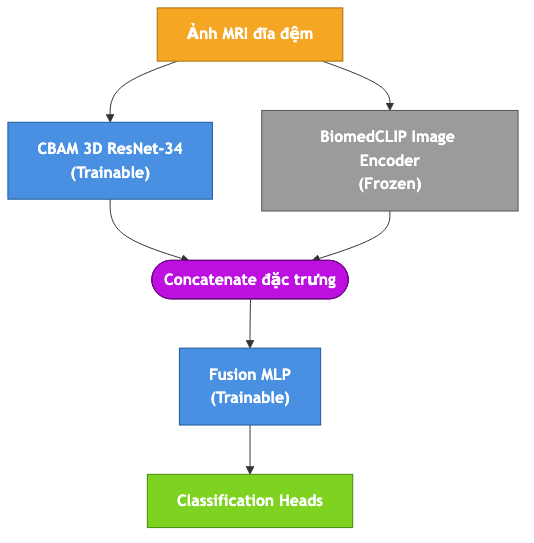
\includegraphics[width=0.5\textwidth]{cslt/hybrid_architecture.png}
    \caption{Kiến trúc Hybrid hai nhánh.}
    \label{fig:hybrid_arch}
\end{figure}

Hình~\ref{fig:training_arch} và Hình~\ref{fig:inference_arch} mô tả riêng biệt hai giai đoạn huấn luyện và suy luận. Trong giai đoạn huấn luyện, dữ liệu đi qua thêm augmentation và minority oversampling; gradient chỉ đi qua nhánh trainable (CBAM-ResNet) còn BiomedCLIP frozen hoàn toàn. Loss tổng hợp gồm Focal Loss và Uncertainty Loss được tính ở các head. Trong giai đoạn suy luận, không có augmentation và loss, chỉ thực hiện forward pass để sinh xác suất dự đoán.

\begin{figure}[htbp]
    \centering
    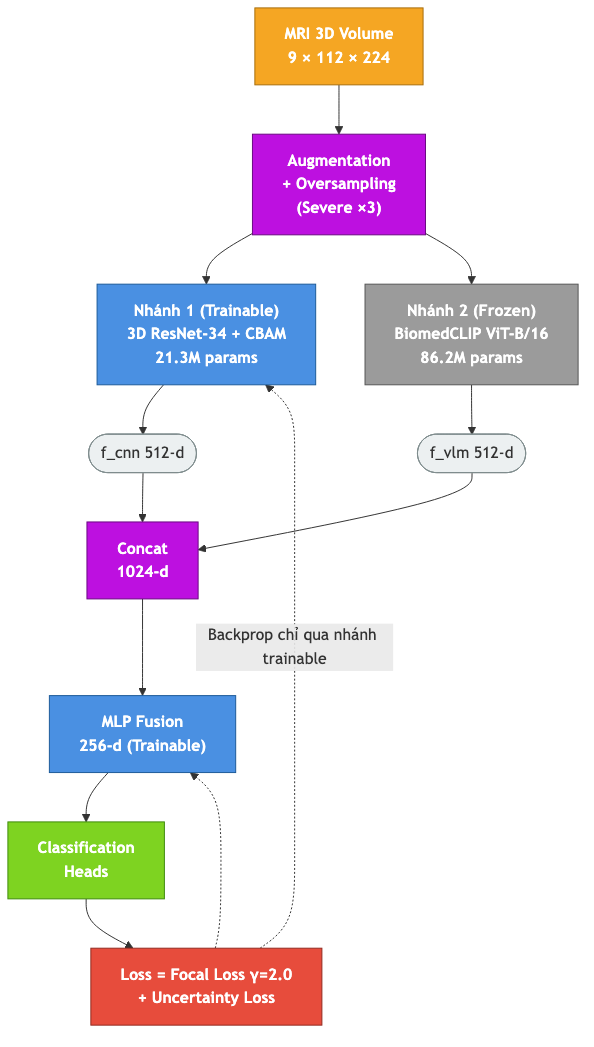
\includegraphics[width=0.58\textwidth]{cslt/training_architecture.png}
    \caption{Kiến trúc huấn luyện.}
    \label{fig:training_arch}
\end{figure}

\begin{figure}[htbp]
    \centering
    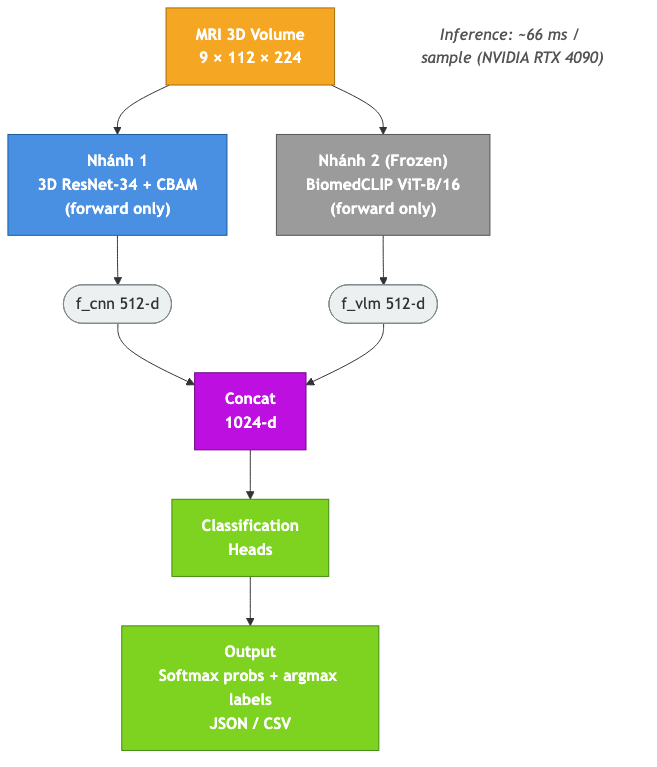
\includegraphics[width=0.6\textwidth]{cslt/inference_architecture.png}
    \caption{Kiến trúc suy luận.}
    \label{fig:inference_arch}
\end{figure}

\subsection{Chi tiết hai nhánh và mô-đun hợp nhất}

\textbf{Nhánh CBAM-3D ResNet-34:} Dựa trên 3D ResNet-34 với convolution 3D kernel $3 \times 3 \times 3$, stride chỉ áp dụng trên hai chiều không gian $(H, W)$ và giữ nguyên chiều slice $D = 9$. Backbone được khởi tạo bằng trọng số pretrained trên Med3D~\cite{chen2019med3d}. Input là khối ảnh đĩa đệm kích thước $(9, 112, 224)$. CBAM được chèn sau mỗi stage của ResNet (4 stages: 64, 128, 256, 512 kênh), vị trí cuối stage là nơi đặc trưng đã đủ trừu tượng để cơ chế chú ý có thể nhìn được pattern ý nghĩa (vùng đĩa đệm tổn thương vs vùng mô lành), nhưng chưa quá nén để mất hết thông tin không gian. Đầu ra sau global average pooling 3D là embedding $f_{cnn}$ 512-d.


\textbf{Nhánh BiomedCLIP:} Cung cấp \emph{prior tổng quát} từ pretraining quy mô lớn. Báo cáo chọn BiomedCLIP \cite{zhang2024biomedclip} thay vì MedCLIP hoặc PMC-CLIP vì BiomedCLIP có dataset pretraining lớn nhất (15M cặp PubMed) và đa dạng modality (MRI, CT, X-ray, mô bệnh học). 

\textbf{Fusion MLPvà heads phân loại:} Hai embedding $f_{cnn}$ và $f_{vlm}$ (mỗi cái 512-d) được ghép thành vector 1024-d, đi qua MLP hai lớp (hidden 256, ReLU, dropout 0.3) cho ra embedding chia sẻ $f_{shared}$ 256-d. Concat + MLP đơn giản hơn các cơ chế gating phức tạp nhưng đủ cho dataset quy mô vừa. 

\subsection{Pipeline xử lý mất cân bằng lớp}
Bài toán RSNA có phân bố nhãn rất mất cân bằng: trên trục Severity, Normal/Mild chiếm $\sim$78\%, Moderate $\sim$18\%, Severe chỉ $\sim$4\%. Mô hình baseline huấn luyện với Cross-Entropy thuần thường rơi vào trạng thái lười, chỉ học dự đoán Normal/Mild để đạt accuracy cao, trong khi Severe Recall gần như bằng 0. Báo cáo áp dụng ba kĩ thuật phối hợp để xử lý vấn đề này:

\textbf{(a) Focal Loss \cite{lin2017focal}.} Giảm trọng số đóng góp của các mẫu dễ (mẫu Normal/Mild đã có xác suất dự đoán $p_t$ cao) và tăng cho các mẫu khó (Severe có $p_t$ thấp). Công thức:
\begin{equation}
    FL(p_t) = -\alpha_t (1 - p_t)^\gamma \log(p_t)
\end{equation}
với $\gamma = 2.0$ là hyperparameter chuẩn. 

\textbf{(b) Uncertainty Loss \cite{kendall2018multitask}.} Học trọng số động giữa các nhãn. Mỗi nhiệm vụ có một tham số log-variance $\sigma_k$ được học cùng với weight của model. Loss tổng cho 5 nhiệm vụ:
\begin{equation}
    \mathcal{L}_{total} = \sum_{k=1}^{5} \left( \frac{1}{2 \sigma_k^2} \mathcal{L}_k + \log \sigma_k \right)
\end{equation}
Nếu một nhiệm vụ có loss cao (ví dụ subarticular stenosis khó hơn các nhãn khác), tham số $\sigma_k$ sẽ tự động tăng lên để giảm trọng số cho nhiệm vụ đó. Cơ chế này ngăn nhiệm vụ khó áp đảo và làm bias các nhiệm vụ dễ hơn.

\textbf{(c) Minority oversampling.} Với mỗi epoch, các sample chứa ít nhất một head có nhãn Severe sẽ được lặp lại 3 lần (oversample factor = 3). Cách này làm tăng đáng kể số iteration mà model thấy các mẫu Severe, từ đó cải thiện khả năng học của lớp hiếm. Hệ số oversampling được điều chỉnh thực nghiệm, giá trị quá cao (5 - 10) gây overfitting trên các mẫu Severe ít ỏi, giá trị quá thấp (1 - 2) không đủ tác động.


\clearpage

\chapter{THỰC NGHIỆM VÀ ĐÁNH GIÁ MÔ HÌNH}

\section{Mô tả dữ liệu và môi trường thực nghiệm}

Để đảm bảo tính khách quan và khả năng ứng dụng thực tế, các thực nghiệm trong nghiên cứu này được tiến hành trên nền tảng đám mây với nguồn dữ liệu đa dạng và độc lập. Phần dưới đây mô tả chi tiết về cấu hình phần cứng, phần mềm và đặc tả các bộ dữ liệu được sử dụng.

\subsection{Môi trường thực nghiệm}
Toàn bộ quá trình huấn luyện và đánh giá được thực hiện trên nền tảng cloud \textbf{Vast.ai}, thuê GPU theo giờ để đảm bảo nguồn lực tính toán đủ mạnh cho training 3D.
\begin{itemize}
    \item \textbf{Phần cứng:} NVIDIA RTX 4090 (24GB VRAM), CUDA 12.x, $\sim$60GB RAM, ổ NVMe.
    \item \textbf{Framework:} PyTorch 2.0+, Python 3.10.
    \item \textbf{Thư viện chính:} SimpleITK, pydicom, OpenCV, scikit-learn, numpy.
\end{itemize}

\subsection{Tập dữ liệu RSNA 2024 Lumbar Spine Degenerative Classification \cite{rsna2024dataset}}
Đây là tập dữ liệu chủ đạo dùng để huấn luyện và đánh giá mô-đun grading. Bộ dữ liệu được tổ chức bởi Hiệp hội X-Quang Bắc Mỹ (RSNA) phối hợp cùng Hiệp hội Thần kinh học Hoa Kỳ (ASNR).

\begin{itemize}
    \item \textbf{Nguồn gốc và quy mô:} Dữ liệu được thu thập từ 8 trung tâm y tế lớn trên 5 châu lục, đảm bảo tính đa dạng về quần thể bệnh nhân và thiết bị chụp. Nhãn dữ liệu được gán thủ công bởi hơn 50 chuyên gia chẩn đoán hình ảnh. Train split $\sim$1\,800 patients (4 fold), val split $\sim$225 patients; mỗi patient có nhiều series MRI (Sagittal T2/STIR, Sagittal T1, Axial T2).
    \item \textbf{Đầu vào:} Ảnh MRI cột sống thắt lưng, định dạng chuẩn DICOM (mỗi series có hàng chục lát sagittal/axial). Quá trình tiền xử lý trích xuất \emph{khối ảnh đĩa đệm 3D} (per-IVD volume) quanh tâm mỗi đĩa đệm, resample về kích thước thống nhất $D \times H \times W = 9 \times 112 \times 224$ (float32), với $D = 9$ lát sagittal trung tâm theo chuẩn của SpineNetV2~\cite{windsor2022spinenetv2}, đủ bao phủ chiều dày đĩa đệm và mô lân cận, cân bằng giữa độ phủ giải phẫu và chi phí tính toán.
    \item \textbf{Nhãn bệnh lý:} Phân loại 5 tình trạng thoái hóa tại 5 tầng đĩa đệm (từ L1/L2 đến L5/S1):
        \begin{itemize}
            \item[$\circ$] Left Neural Foraminal Narrowing
            \item[$\circ$] Right Neural Foraminal Narrowing
            \item[$\circ$] Left Subarticular Stenosis
            \item[$\circ$] Right Subarticular Stenosis
            \item[$\circ$] Spinal Canal Stenosis
        \end{itemize}
    \item \textbf{Hệ thống phân cấp:} Mức độ nghiêm trọng được chia thành 3 cấp: Normal/Mild, Moderate, Severe.
    \item \textbf{Phân bố lớp (mất cân bằng):} Lớp Severe chỉ chiếm $\sim$4\% mẫu trong khi Normal/Mild chiếm $\sim$81\%, nguồn gốc bài toán mất cân bằng. Hình~\ref{fig:rsna_class_dist} minh họa chi tiết.
    \item \textbf{Vai trò trong nghiên cứu:} Training set chính + validation set để tinh chỉnh mô-đun grading và so sánh 4 cấu hình ablation.
\end{itemize}

\begin{figure}[htbp]
    \centering
    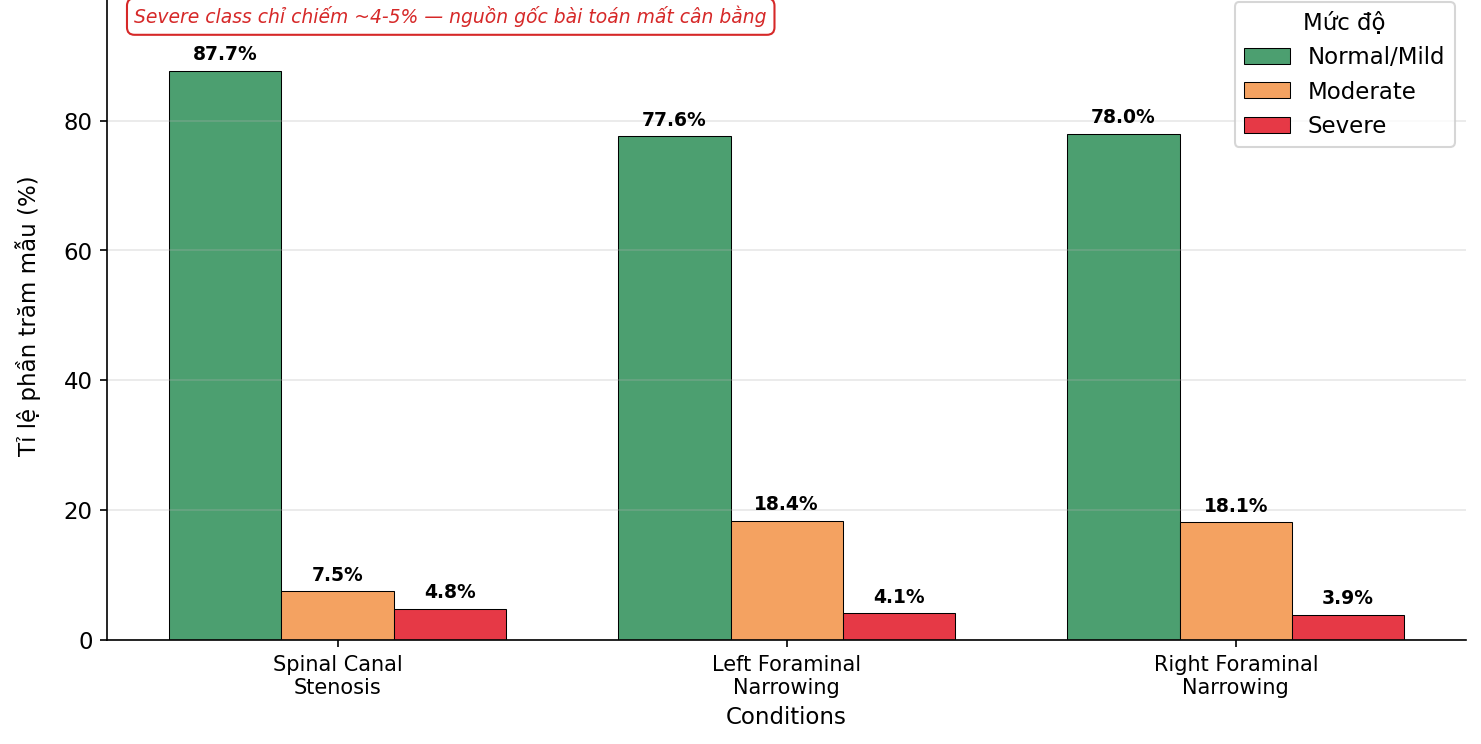
\includegraphics[width=0.95\textwidth]{cslt/rsna_class_distribution.png}
    \caption{Phân bố lớp trên RSNA 2024.}
    \label{fig:rsna_class_dist}
\end{figure}


\subsection{Tập dữ liệu Lumbar Spine Segmentation \cite{chu2015dataset}}
Tập dữ liệu được công bố bởi Chu và cộng sự \cite{chu2015dataset}, có nguồn gốc từ Viện Công nghệ và cơ sinh học phẫu thuật, Đại học Bern (Thụy Sĩ). Trong phạm vi luận văn này, đây đóng vai trò là tập kiểm thử độc lập để đánh giá hiệu năng phân vùng của TotalSpineSeg.

\begin{itemize}
    \item \textbf{Quy mô:} Bao gồm ảnh MRI T2-weighted của 23 bệnh nhân ẩn danh. Mỗi ca chụp chứa ít nhất 7 thân đốt sống thuộc vùng cột sống dưới (từ T11 đến L5).
    \item \textbf{Đặc điểm hình ảnh:} Chuỗi xung Turbo Spin Echo trọng số T2. Dữ liệu được lưu trữ dưới định dạng NIfTI (.nii), giúp bảo toàn thông tin không gian 3D chuẩn y tế.
    \item \textbf{Nhãn phân vùng:}
        \begin{itemize}
            \item[$\circ$] \textbf{Loại nhãn:} Mặt nạ nhị phân.
            \item[$\circ$] \textbf{Đặc điểm:} Nhãn được gán cho toàn bộ vùng cột sống. Khác với các bộ dữ liệu hiện đại thường phân lớp chi tiết từng đốt sống, bộ dữ liệu này gán nhãn gộp cho cấu trúc đốt sống (bao gồm thân đốt sống và thành phần phụ) mà không tách biệt định danh từng đốt sống (L1, L2...).
        \end{itemize}
    \item \textbf{Mục đích sử dụng:} Đánh giá khả năng định vị và phân vùng cột sống trên miền dữ liệu chưa từng thấy, qua đó kiểm chứng độ bền vững của thuật toán phân vùng được chọn.
\end{itemize}

\subsection{Tập dữ liệu SPIDER \cite{vansluijs2022spider}}
Tập dữ liệu SPIDER (van der Graaf và cộng sự, công bố trên Nature Scientific Data 2024) được dùng làm test set độc lập để kiểm chứng khả năng tổng quát hóa cross-dataset của mô-đun grading.

\begin{itemize}
    \item \textbf{Quy mô:} 218 bệnh nhân $\times$ $\sim$5 đĩa đệm $\approx$ 1\,520 IVD samples, hoàn toàn độc lập với RSNA.
    \item \textbf{Định dạng:} Các file MetaImage \texttt{.mha} (đọc qua \texttt{SimpleITK}), kèm segmentation mask 3D với label 201--207 chỉ vị trí từng đĩa đệm.
    \item \textbf{Nhãn bệnh lý (mở rộng so với RSNA):} 8 nhãn theo chuẩn lâm sàng:
        \begin{itemize}
            \item[$\circ$] Pfirrmann grade (5 lớp): thang đo thoái hóa đĩa đệm.
            \item[$\circ$] Modic changes (4 lớp): biến đổi tủy xương dưới sụn.
            \item[$\circ$] Disc narrowing (binary): hẹp đĩa đệm.
            \item[$\circ$] Spondylolisthesis (binary): trượt đốt sống.
            \item[$\circ$] Upper/Lower endplate damage (binary $\times$ 2): tổn thương mặt trên/dưới đốt sống.
            \item[$\circ$] Disc herniation (binary): thoát vị đĩa đệm.
            \item[$\circ$] Disc bulging (binary): phồng đĩa đệm.
        \end{itemize}
    \item \textbf{Phân bố lớp:} Hai nhãn mất cân bằng nghiêm trọng là Spondylolisthesis (2.8\% positive) và Disc herniation (4.7\% positive). Chi tiết ở Hình~\ref{fig:spider_class_dist}.
    \item \textbf{Vai trò trong nghiên cứu:} Test set độc lập cho transfer learning, đánh giá: (i) mô hình huấn luyện trên RSNA có chuyển giao tốt sang dataset khác? (ii) các nhãn mới (Pfirrmann, Modic, \ldots) có học được từ feature backbone đã pretrained không?
\end{itemize}

\begin{figure}[htbp]
    \centering
    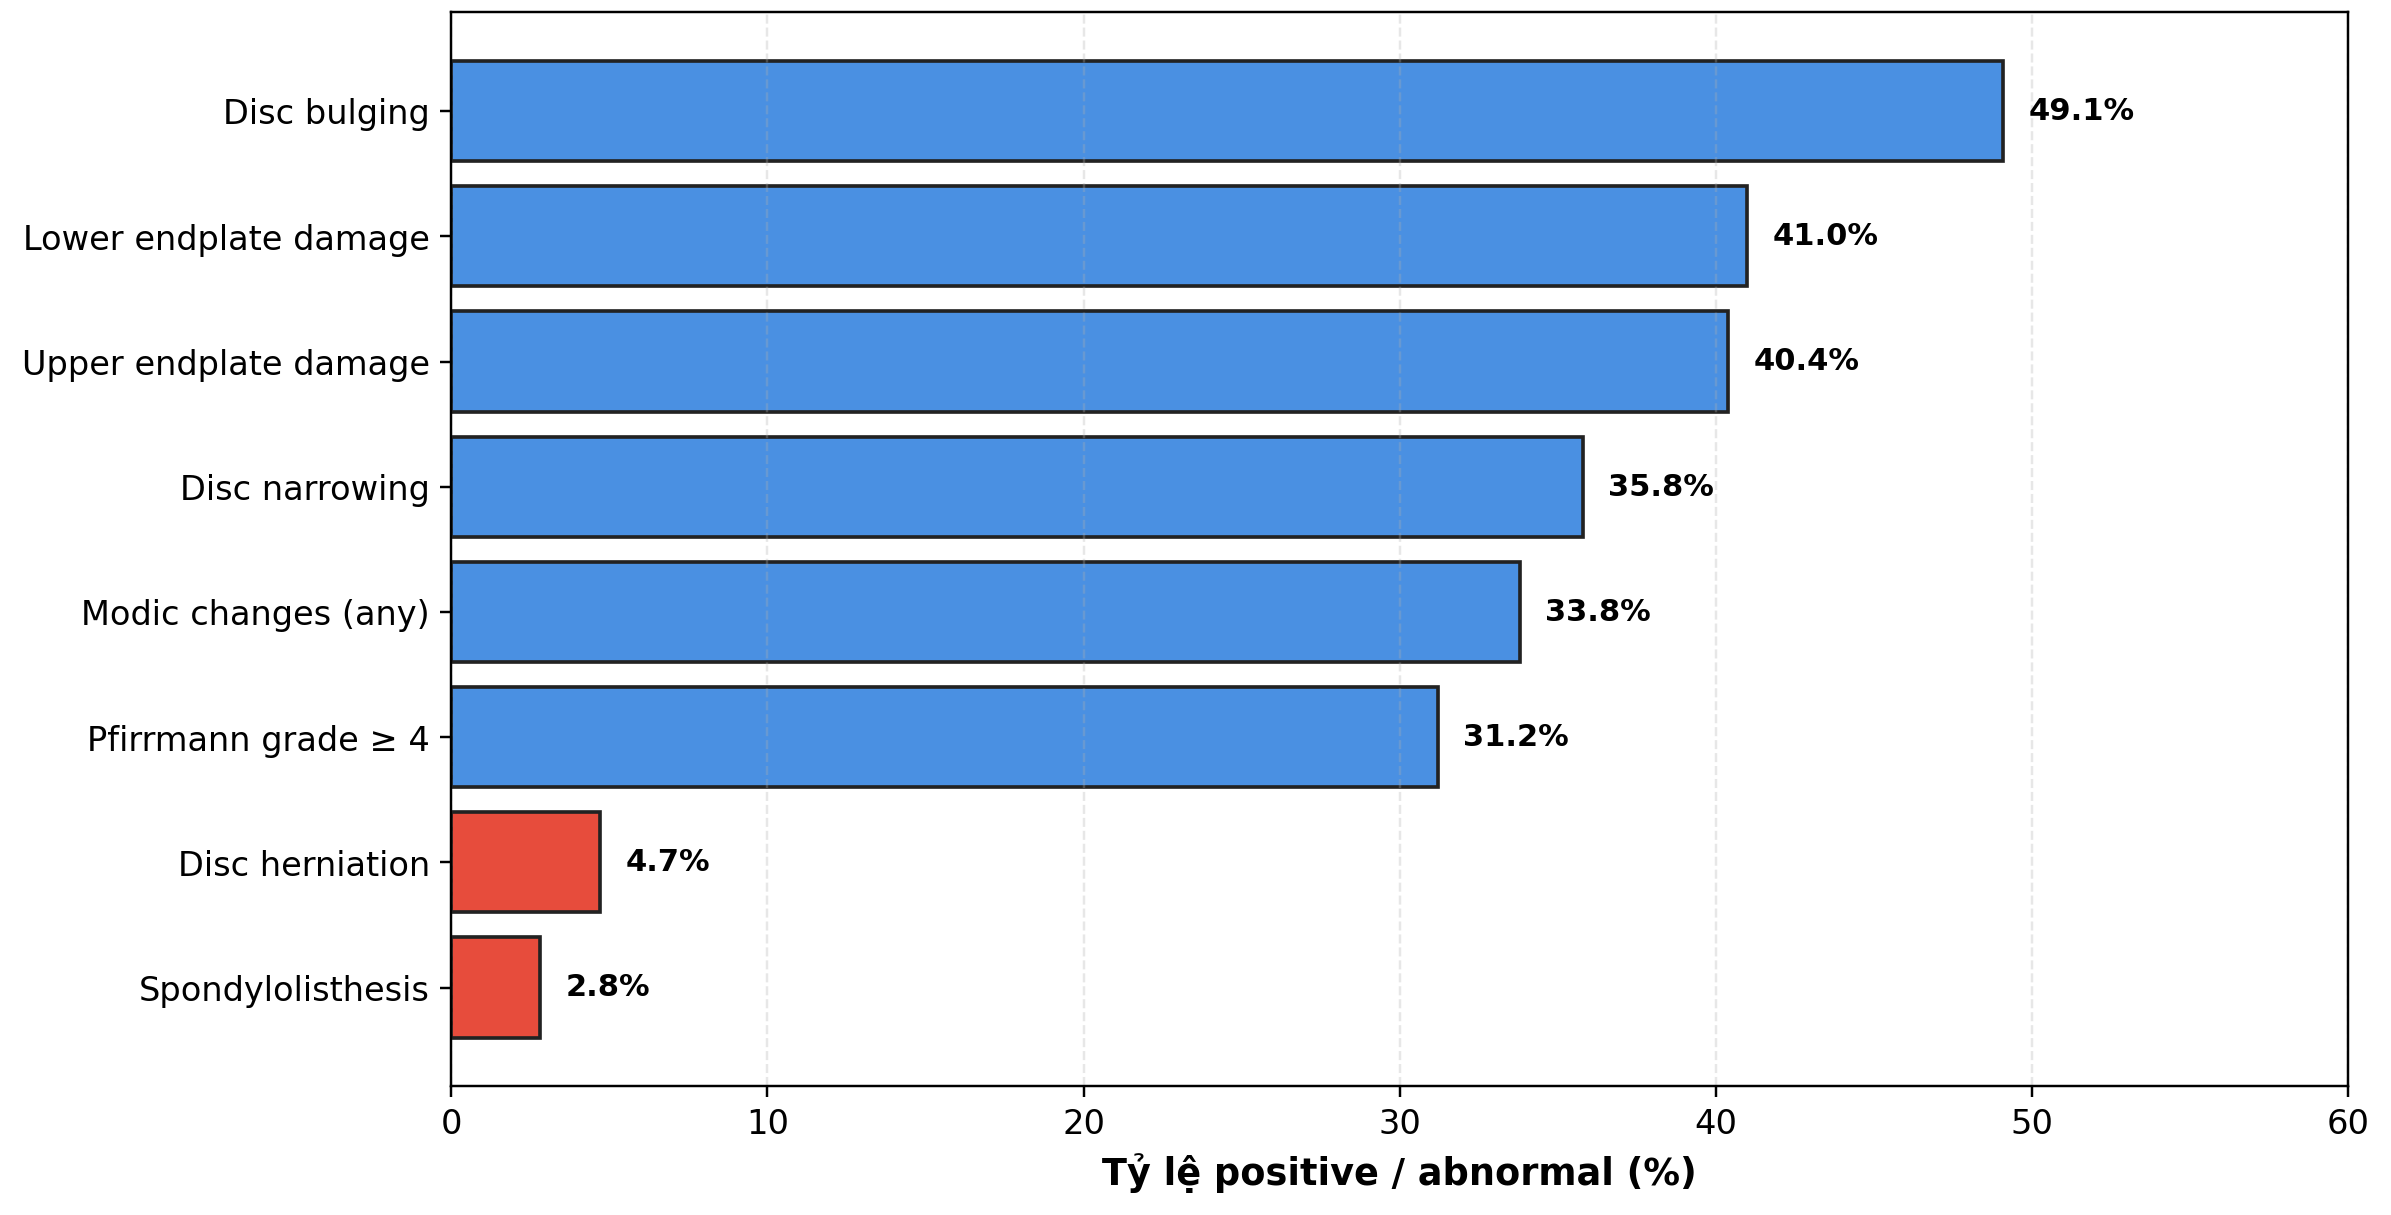
\includegraphics[width=\textwidth]{cslt/spider_class_distribution.png}
    \caption{Phân bố nhãn trên SPIDER 8 conditions.}
    \label{fig:spider_class_dist}
\end{figure}


\section[Thí nghiệm chọn mô-đun phân vùng]{Thí nghiệm chọn mô-đun phân vùng}
\label{sec:eval_segmentation}

\textbf{Mục tiêu thí nghiệm:} chọn 1 trong 4 mô hình phân vùng sẵn có cho pipeline đề xuất. Thí nghiệm so sánh \textbf{TotalSpineSeg} (tối ưu cho thân đốt sống), \textbf{SPINEPS} (tối ưu cho toàn bộ cấu trúc cột sống), \textbf{MedCLIP-SAMv2} (zero-shot text-driven), và \textbf{SpineNetV2} (mô hình spine chuyên dụng) trên tập kiểm thử 23 khối ảnh Ground Truth (vùng từ T11 đến L5).

\subsection{Các tiêu chí đánh giá}
Để đánh giá định lượng chất lượng phân vùng ảnh y tế 3D, nghiên cứu sử dụng các chỉ số tiêu chuẩn sau:

\begin{itemize}
    \item \textbf{Hệ số Dice (Dice Score):} 
    Thước đo phổ biến nhất về độ chồng lắp giữa vùng dự đoán ($P$) và nhãn thực tế ($G$) trong không gian 3D.
    \begin{equation}
        \text{Dice} = \frac{2 \times |P \cap G|}{|P| + |G|}
    \end{equation}

    \item \textbf{Chỉ số IoU (Jaccard Index):}
    Tỷ lệ giữa phần giao và phần hợp của hai tập hợp voxel.
    \begin{equation}
        \text{IoU} = \frac{|P \cap G|}{|P \cup G|}
    \end{equation}

    \item \textbf{Precision và Recall:}
    Đánh giá độ chính xác và độ bao phủ của mô hình.
    \begin{equation}
        \text{Precision} = \frac{TP}{TP + FP}, \quad \text{Recall} = \frac{TP}{TP + FN}
    \end{equation}
    \textit{Trong đó $TP$, $FP$, $FN$ lần lượt là số lượng voxel dự đoán đúng, dự đoán thừa và bỏ sót.}

    \item \textbf{Average Symmetric Surface Distance (ASSD):}
    Đây là chỉ số đánh giá độ sai lệch trung bình giữa bề mặt 3D của vùng dự đoán ($\partial P$) và bề mặt thực tế ($\partial G$). Chỉ số này được tính bằng trung bình cộng khoảng cách từ tất cả các điểm trên bề mặt dự đoán đến bề mặt thực tế và ngược lại.
    \begin{equation}
        \text{ASSD} = \frac{1}{|\partial P| + |\partial G|} \left( \sum_{p \in \partial P} d(p, \partial G) + \sum_{g \in \partial G} d(g, \partial P) \right)
    \end{equation}
    \textit{Trong đó $d(x, S)$ là khoảng cách Euclid ngắn nhất từ điểm $x$ đến bề mặt $S$ trong không gian 3 chiều. Giá trị ASSD càng nhỏ chứng tỏ bề mặt tái tạo càng chính xác.}
\end{itemize}

\subsection{Kết quả thực nghiệm}
Bảng \ref{tab:seg_results} trình bày kết quả so sánh trung bình trên 4 mô hình. \textbf{TotalSpineSeg} đạt hiệu năng tổng thể cao nhất với chỉ số Dice (70.81\%) và Precision (97.87\%). \textbf{SpineNetV2} đạt kết quả Dice Score 67.82\% và có chỉ số Recall cao nhất bảng (91.79\%). Đối với mô hình zero-shot \textbf{MedCLIP-SAMv2}, mặc dù Recall đạt mức cao nhưng độ chính xác biên dạng còn hạn chế.

\begin{table}[h!]
    \centering
    \caption{So sánh hiệu năng phân vùng giữa TotalSpineSeg, SPINEPS, MedCLIP-SAMv2 và SpineNetV2}
    \label{tab:seg_results}
    \renewcommand{\arraystretch}{1.2}
    \setlength{\tabcolsep}{4pt}
    \begin{tabular}{lcccc}
        \toprule
        \textbf{Tiêu chí} & \textbf{TotalSpineSeg} & \textbf{SPINEPS} & \textbf{MedCLIP-SAMv2} & \textbf{SpineNetV2} \\
        \midrule
        \textbf{Dice Score} & \textbf{70.81\%} & 58.68\% & 40.55\% & 67.82\% \\
        \textbf{IoU} & \textbf{55.74\%} & 41.56\% & 26.47\% & 51.41\% \\
        \textbf{Precision}  & \textbf{97.87\%} & 52.17\% & 29.16\% & 51.76\% \\
        \textbf{Recall}  & 56.49\% & 68.34\% & \textbf{91.98\%} & 91.79\% \\
        \textbf{ASSD}  & \textbf{6.85 mm} & 7.48 mm & 19.50 mm & 8.04 mm \\
        \bottomrule
    \end{tabular}
\end{table}

\subsection{Phân tích và thảo luận}

\subsubsection{Lý giải sự chênh lệch giữa Recall và Precision}
Kết quả thực nghiệm cho thấy sự khác biệt về đặc tính của từng mô hình, xuất phát từ thiết kế và định nghĩa nhãn thực tế:

\begin{itemize}
    \item \textbf{Vấn đề về ground truth:} Dữ liệu ground truth bao gồm toàn bộ đốt sống (thân + gai sau + mỏm ngang).
    \item \textbf{TotalSpineSeg:} Được thiết kế tập trung vào \textbf{thân đốt sống}, do đó mô hình chủ động bỏ qua các phần gai sau, dẫn đến Recall ở mức 56.49\%. Tuy nhiên, độ chính xác trên vùng thân đốt sống đạt mức rất cao (Precision 97.87\%) và ít nhiễu.
    \item \textbf{SpineNetV2:} Đạt chỉ số Recall 91.79\% nhờ chiến lược tối đa hóa vùng bao phủ. Mô hình có xu hướng tạo ra vùng dự đoán rộng để đảm bảo độ chồng lấn cao nhất với dữ liệu nhãn, ưu tiên việc phát hiện đầy đủ đối tượng hơn là tối ưu hóa biên dạng giải phẫu chi tiết như các mô hình phân vùng chuyên biệt.
    \item \textbf{SPINEPS \& MedCLIP-SAMv2:} Cả hai mô hình đều có Precision thấp (dưới 53\%), cho thấy hiện tượng phân vùng thừa (over-segmentation) so với nhãn mục tiêu. Riêng MedCLIP-SAMv2 có sai số biên dạng lớn nhất (ASSD 19.50mm).
\end{itemize}
\subsubsection{Lựa chọn mô hình cho hệ thống đề xuất}
Dựa trên mục tiêu xây dựng hệ thống hỗ trợ chẩn đoán (yêu cầu xác định chính xác vị trí thân đốt sống để trích xuất ảnh), nghiên cứu lựa chọn \textbf{TotalSpineSeg} vì các lý do sau:

\begin{enumerate}
    \item \textbf{Độ tin cậy cao:} Precision 97.87\% đảm bảo vùng được xác định là đốt sống với độ chính xác cao, hạn chế nhiễu trong các bước xử lý tiếp theo, cao hơn đáng kể so với mức ~51\% của SpineNetV2 và SPINEPS.
    \item \textbf{Độ chính xác bề mặt 3D:} Chỉ số ASSD thấp (6.85mm) cho thấy khả năng tái tạo bề mặt thân đốt sống bám sát giải phẫu thực tế, tốt hơn so với MedCLIP-SAMv2 và SPINEPS.
    \item \textbf{Tính ổn định:} Độ lệch chuẩn thấp ($\pm 5.23\%$) cho thấy sự ổn định khi áp dụng trên dữ liệu lâm sàng. Mặc dù SpineNetV2 có Recall tốt hơn, nhưng Precision thấp khiến mô hình này phù hợp hơn cho bài toán phát hiện thay vì phân vùng chính xác cho phẫu thuật.
\end{enumerate}


\section{Thí nghiệm chọn mô-đun đánh giá phát hiện bất thường}
\label{sec:eval_detection}

\textbf{Mục tiêu thí nghiệm:} Chọn 1 trong 3 mô hình sẵn có làm backbone cho mô-đun grading trong pipeline đề xuất. Thí nghiệm so sánh các mô hình ở góc nhìn binary detection (có/không bệnh) trên RSNA val 150 bệnh nhân để xác định: (i) mô hình nào đủ chính xác và ổn định cho clinical screening, (ii) mô hình nào có kiến trúc đủ đơn giản và mã nguồn mở để có thể tinh chỉnh tiếp ở thí nghiệm xác thực đóng góp (Mục~\ref{sec:phase2_eval}).

Thực nghiệm được tiến hành so sánh giữa ba mô hình đại diện:
\begin{itemize}
    \item \textbf{SpineNetV2:} Mô hình mã nguồn mở với khả năng gán nhãn đa dạng (9-10 clinical features).
    \item \textbf{MedGemma:} Mô hình ngôn ngữ - thị giác lớn (VLM).
    \item \textbf{Ning Shen:} Giải pháp đạt giải nhất cuộc thi RSNA 2024 (SOTA Baseline).
\end{itemize}
\subsection{Các tiêu chí đánh giá}
Để đánh giá hiệu năng của các mô hình trên tập dữ liệu RSNA 2024 (bao gồm 150 bệnh nhân), nghiên cứu sử dụng các chỉ số phổ biến trong bài toán phân loại y tế: Accuracy, Precision, Recall và F1-Score.

Gọi $TP$ (True Positive) là số mẫu dương tính được dự đoán đúng, $TN$ (True Negative) là số mẫu âm tính được dự đoán đúng, $FP$ (False Positive) là số mẫu âm tính bị dự đoán sai thành dương tính, và $FN$ (False Negative) là số mẫu dương tính bị dự đoán sai thành âm tính. Các công thức được định nghĩa như sau:

\begin{equation}
    \text{Accuracy} = \frac{TP + TN}{TP + TN + FP + FN}
\end{equation}

\begin{equation}
    \text{Precision} = \frac{TP}{TP + FP}
\end{equation}

\begin{equation}
    \text{Recall} = \frac{TP}{TP + FN}
\end{equation}

\begin{equation}
    \text{F1-Score} = 2 \times \frac{\text{Precision} \times \text{Recall}}{\text{Precision} + \text{Recall}}
\end{equation}

\textbf{Per-class F1 (Severe F1, Moderate F1, Normal F1).} Khi bài toán có nhiều lớp (Normal/Mild, Moderate, Severe), 4 chỉ số ở trên có thể tính \emph{riêng cho từng lớp} (theo cách one-vs-rest). Ví dụ \textit{Severe F1} chỉ tính trên các mẫu thuộc lớp Severe --- đặc biệt quan trọng cho bài toán mất cân bằng vì class hiếm dễ bị ``che lấp'' bởi class chiếm đa số.

\textbf{Mean F1 macro.} Trung bình cộng F1 trên tất cả các lớp, mỗi lớp có trọng số bằng nhau:
\begin{equation}
    \text{F1}_{\text{macro}} = \frac{1}{K} \sum_{k=1}^{K} \text{F1}_k
\end{equation}
với $K$ là số lớp. Khác với F1 weighted (lấy trung bình theo tần suất class), F1 macro \emph{phạt mạnh các class hiếm có hiệu năng thấp}, phù hợp cho clinical screening vì các ca Severe quan trọng nhưng số lượng ít.

\textbf{AUC (Area Under ROC Curve).} Diện tích dưới đường cong ROC, biểu diễn quan hệ giữa True Positive Rate (Recall) và False Positive Rate khi thay đổi ngưỡng quyết định. AUC = 0.5 tương đương dự đoán ngẫu nhiên, AUC = 1.0 là phân loại hoàn hảo. \emph{Ưu điểm:} không phụ thuộc ngưỡng phân loại, đánh giá chất lượng ranking của xác suất dự đoán.
\begin{equation}
    \text{AUC} = \int_0^1 \text{TPR}(\text{FPR}^{-1}(t)) \, dt
\end{equation}

\textbf{AUPRC (Area Under Precision-Recall Curve).} Diện tích dưới đường cong Precision-Recall. Phù hợp hơn AUC cho dữ liệu \emph{mất cân bằng nghiêm trọng}: AUC có thể trông cao một cách giả tạo khi class majority quá lớn, trong khi AUPRC tập trung vào hiệu năng của class hiếm (positive class). Báo cáo sử dụng AUPRC làm chỉ số chính cho lớp Severe.
\begin{equation}
    \text{AUPRC} = \int_0^1 \text{Precision}(\text{Recall}^{-1}(t)) \, dt
\end{equation}

\subsection{Kết quả thực nghiệm}

Ba mô hình được đánh giá trên tập validation gồm 150 bệnh nhân, bao gồm ba nhóm bệnh lý chính: Hẹp ống sống, hẹp lỗ liên hợp trái, và hẹp lỗ liên hợp phải. Các chỉ số precision, recall, và F1-score được sử dụng để đánh giá khả năng phát hiện bất thường của từng mô hình.

\textbf{a. Hẹp ống sống}

Bảng~\ref{tab:scs_metrics} trình bày chi tiết kết quả của nhóm này. Kết quả cho thấy đây là nhóm bệnh lý có tỷ lệ phát hiện tốt nhất. Ning Shen đạt F1-Score 81.20\% với precision 81.82\% và recall 80.60\%, cho thấy model này phát hiện khá chính xác và ít bỏ sót. SpineNetV2 đạt F1-Score 78.79\% với recall 80.00\%, cũng thể hiện khả năng phát hiện tốt. MedGemma có F1-Score thấp hơn nhiều (31.17\%) do recall chỉ 20.87\%, nghĩa là bỏ sót gần 80\% bệnh nhân có bệnh hẹp ống sống.

\begin{table}[h!]
    \centering
    \caption{Kết quả chi tiết nhóm Hẹp ống sống}
    \label{tab:scs_metrics}
    \renewcommand{\arraystretch}{1.2}
    \begin{tabular}{lcccc}
        \toprule
        \textbf{Mô hình} & \textbf{Accuracy} & \textbf{Precision} & \textbf{Recall} & \textbf{F1-Score} \\
        \midrule
        Ning Shen & \textbf{86.63\%} & \textbf{81.82\%} & \textbf{80.60\%} & \textbf{81.20\%} \\
        SpineNetV2 & 81.58\% & 77.61\% & 80.00\% & 78.79\% \\
        MedGemma & 29.33\% & 61.54\% & 20.87\% & 31.17\% \\
        \bottomrule
    \end{tabular}
\end{table}

\textbf{b. Hẹp lỗ liên hợp trái}

Bảng~\ref{tab:nfn_left_metrics} trình bày chi tiết kết quả của nhóm này. Ning Shen đạt F1-Score 79.43\% với Recall cao (87.37\%), phù hợp với yêu cầu của screening là cần ưu tiên phát hiện được nhiều trường hợp bị bệnh. SpineNetV2 cũng có Recall cao (84.00\%) và F1-Score 77.30\%, cho thấy sự cân bằng khá tốt giữa khả năng phát hiện và độ chính xác. MedGemma có hiệu năng kém hơn với F1-Score 13.86\% do Recall chỉ 8.43\%, tức là bỏ sót hơn 91\% bệnh nhân bị bệnh Hẹp lỗ liên hợp trái.

\begin{table}[h!]
    \centering
    \caption{Kết quả chi tiết nhóm Hẹp lỗ liên hợp trái}
    \label{tab:nfn_left_metrics}
    \renewcommand{\arraystretch}{1.2}
    \begin{tabular}{lcccc}
        \toprule
        \textbf{Mô hình} & \textbf{Accuracy} & \textbf{Precision} & \textbf{Recall} & \textbf{F1-Score} \\
        \midrule
        Ning Shen & \textbf{77.01\%} & \textbf{72.81\%} & \textbf{87.37\%} & \textbf{79.43\%} \\
        SpineNetV2 & 75.66\% & 71.59\% & 84.00\% & 77.30\% \\
        MedGemma & 42.00\% & 38.89\% & 8.43\% & 13.86\% \\
        \bottomrule
    \end{tabular}
\end{table}

\textbf{c. Hẹp lỗ liên hợp phải}

Bảng~\ref{tab:nfn_right_metrics} trình bày chi tiết kết quả của nhóm này. Ning Shen có F1-Score 81.48\% và Recall 84.62\%, thể hiện sự ổn định trên các nhóm bệnh lý khác nhau. SpineNetV2 đạt F1-Score 76.40\% với Precision và Recall khá cân bằng (75.56\% và 77.27\%). MedGemma có kết quả thấp nhất với F1-Score 10.75\% và Recall cực kỳ thấp (6.02\%), bỏ sót gần 94\% bệnh nhân bị Hẹp lỗ liên hợp phải. Điều này chứng tỏ MedGemma có xu hướng dự đoán quá an toàn (thiên về kết quả bình thường), do đó không đáp ứng được yêu cầu của việc sàng lọc

\begin{table}[h!]
    \centering
    \caption{Kết quả chi tiết nhóm Hẹp lỗ liên hợp phải}
    \label{tab:nfn_right_metrics}
    \renewcommand{\arraystretch}{1.2}
    \begin{tabular}{lcccc}
        \toprule
        \textbf{Mô hình} & \textbf{Accuracy} & \textbf{Precision} & \textbf{Recall} & \textbf{F1-Score} \\
        \midrule
        Ning Shen & \textbf{78.61\%} & \textbf{78.57\%} & \textbf{84.62\%} & \textbf{81.48\%} \\
        SpineNetV2 & 72.37\% & 75.56\% & 77.27\% & 76.40\% \\
        MedGemma & 44.67\% & 50.00\% & 6.02\% & 10.75\% \\
        \bottomrule
    \end{tabular}
\end{table}

\subsection{Phân tích và thảo luận}

\textbf{Hiệu năng: }Nhìn chung, Ning Shen có hiệu năng tốt nhất với F1-Score trung bình 80.37\% và khá ổn định trên cả ba nhóm bệnh lý (từ 79.43\% đến 81.48\%). Kết quả này phù hợp với kỳ vọng từ một SOTA model được thiết kế riêng cho RSNA 2024 dataset. SpineNetV2 đạt F1-Score trung bình 77.50\%, thấp hơn Ning Shen khoảng 3\%, nhưng vẫn cho thấy khả năng detection khá tốt với performance ổn định (76.40\% - 78.79\%). MedGemma có F1-Score trung bình thấp nhất (18.59\%), chủ yếu do Recall quá thấp (6.02\% - 20.87\%) ở tất cả các conditions. \\

\textbf{Về recall và precision trong bài toán sàng lọc}: 
Kết quả thực nghiệm cho thấy một xu hướng rõ rệt ở NingShen và SpineNetV2 là việc ưu tiên độ nhạy (Recall, đạt $80-87\%$) hơn so với độ chính xác (Precision, đạt $72-82\%$). Chiến lược này hoàn toàn phù hợp với nguyên tắc cốt lõi của bài toán sàng lọc y tế: tối thiểu hóa tỷ lệ bỏ sót bệnh (False negatives) ngay cả khi phải chấp nhận gia tăng tỷ lệ báo động giả (False positives). Trong thực tế lâm sàng, các cảnh báo giả có thể dễ dàng được bác sĩ loại bỏ qua quá trình kiểm tra chi tiết, nhưng việc bỏ sót một bệnh nhân có bệnh lại gây ra hậu quả nghiêm trọng hơn nhiều.\\

Trái lại, MedGemma thể hiện chiến lược dự đoán thận trọng quá mức. Mặc dù chỉ số Precision đạt mức chấp nhận được ($38.89\% - 61.54\%$), chỉ số Recall lại cực thấp ($6.02\% - 20.87\%$), đồng nghĩa với việc mô hình đã bỏ sót tới $80-94\%$ số ca bệnh thực tế. Điều này khẳng định rằng MedGemma, với bản chất là một mô hình VLM đa dụng chưa được tinh chỉnh cho dữ liệu cột sống thắt lưng, do đó không đáp ứng được yêu cầu của tác vụ sàng lọc.\\

\textbf{Độ ổn định giữa các nhóm bệnh:} Ning Shen có độ ổn định cao với F1-Score dao động ít (81.20\% - 81.48\% cho hai bệnh Hẹp lỗ liên hợp phải, hẹp ống sống, 79.43\% cho hẹp lỗ liên hợp trái). SpineNetV2 cũng khá ổn định (76.40\% - 78.79\%). Ngược lại, MedGemma có variance cao (10.75\% - 31.17\%), cho thấy performance không đồng đều và đặc biệt kém với Hẹp lỗ liên hợp phải. \\

\textbf{Mô hình được chọn:} \textbf{SpineNetV2} được chọn làm backbone cho mô-đun grading vì cân bằng tốt nhất giữa độ chính xác (F1 trung bình 77.50\%, chỉ thấp hơn Ning Shen 3\%) và tính khả thi triển khai (mã nguồn mở, kiến trúc 3D ResNet-34 đơn giản, dễ tinh chỉnh). Ning Shen có F1 cao hơn nhưng là ensemble nhiều mô hình lớn, khó duy trì và không phù hợp với pipeline thực tế của báo cáo. MedGemma bị loại do Recall quá thấp (6--21\%). \\

 Khi phân tích sâu hơn theo từng \emph{cấp độ bệnh} trên full RSNA, SpineNetV2 baseline có Severe Recall chỉ 12.3\%, gần 9/10 ca nặng bị bỏ sót, mặc dù detection-level F1 vẫn 77.50\%. Điểm yếu này là động cơ trực tiếp cho thí nghiệm tiếp theo: tinh chỉnh mô-đun grading bằng CBAM + BiomedCLIP để cải thiện cụ thể trên Severe class.

\section[Thí nghiệm xác thực đóng góp tinh chỉnh]{Thí nghiệm xác thực đóng góp tinh chỉnh}
\label{sec:phase2_eval}

{Mục tiêu thí nghiệm nhằm xác thực rằng các đóng góp tinh chỉnh (CBAM attention + BiomedCLIP frozen + pipeline xử lý mất cân bằng) thật sự cải thiện hiệu năng so với backbone đã chọn ở Mục~\ref{sec:eval_detection}. Thí nghiệm dựng 4 cấu hình ablation (SpineNetV2 / +CBAM / BMC-only / Hybrid) trên RSNA 2024 full train+val, đồng thời kiểm chứng tổng quát hóa qua transfer learning sang SPIDER 8-label với 3-seed evaluation.


\subsection{Thiết lập huấn luyện}
Toàn bộ thực nghiệm chạy trên NVIDIA RTX 4090 (24GB VRAM) trên Vast.ai cloud instance. Framework PyTorch 2.0+, Python 3.10.

% \begin{table}[h!]
% \centering
% \caption{Hyperparameter 4 cấu hình ablation.}
% \label{tab:phase2_hyperparams}
% \renewcommand{\arraystretch}{1.2}
% \setlength{\tabcolsep}{4pt}
% \begin{tabular}{lcccc}
% \toprule
% \textbf{Hyperparameter} & \textbf{SpineNetV2} & \textbf{CBAM} & \textbf{BMC-only} & \textbf{Hybrid} \\
% \midrule
% Optimizer & AdamW & AdamW & AdamW & AdamW \\
% Learning rate & 1e-3 & 1e-3 & 1e-3 & 1e-3 \\
% Batch size & 32 & 32 & 32 & 32 \\
% Epochs (RSNA) & 30 & 20 & 25 & 25 \\
% Augmentation & medium & medium & medium & medium \\
% Oversample factor & 3 & 3 & 3 & 3 \\
% Loss & FocalLoss + UncertaintyLoss & --- & --- & --- \\
% BiomedCLIP frozen & N/A & N/A & Yes & Yes \\
% \bottomrule
% \end{tabular}
% \end{table}

Bốn cấu hình ablation được định nghĩa: (i) \textbf{SpineNetV2} - chỉ 3D ResNet-34 không có CBAM, không có BiomedCLIP; (ii) \textbf{CBAM} - thêm CBAM vào ResNet-34, không có BiomedCLIP; (iii) \textbf{BMC-only} - bỏ ResNet-34, chỉ dùng BiomedCLIP frozen với linear classifier; (iv) \textbf{Hybrid} - CBAM-ResNet-34 + BiomedCLIP frozen, fusion qua MLP.



\subsection{Kết quả trên RSNA 2024}
\label{subsec:rsna_ablation}

Bảng~\ref{tab:rsna_ablation} tổng hợp kết quả của 4 cấu hình ablation trên RSNA 2024.

\begin{table}[htbp]
\centering
\caption{Kết quả 4 cấu hình trên RSNA 2024, trung bình $\pm$ độ lệch chuẩn qua 3 hạt giống ngẫu nhiên 42, 123 và 456.}
\label{tab:rsna_ablation}
\renewcommand{\arraystretch}{1.2}
\setlength{\tabcolsep}{4pt}
\begin{tabular}{lcccc}
\toprule
\textbf{Chỉ số} & \textbf{SpineNetV2} & \textbf{CBAM} & \textbf{BMC-only} & \textbf{Hybrid} \\
\midrule
Mean F1 (macro)        & 0.420 $\pm$ 0.010 & 0.477 $\pm$ 0.057 & 0.482 $\pm$ 0.019 & \textbf{0.527 $\pm$ 0.027} \\
Mean Recall (macro)    & 0.412 $\pm$ 0.005 & 0.531 $\pm$ 0.068 & 0.532 $\pm$ 0.004 & \textbf{0.592 $\pm$ 0.026} \\
Mean Precision (macro) & 0.493 $\pm$ 0.028 & 0.499 $\pm$ 0.037 & 0.508 $\pm$ 0.037 & \textbf{0.526 $\pm$ 0.013} \\
Mean AUC               & 0.835 $\pm$ 0.010 & 0.803 $\pm$ 0.050 & 0.826 $\pm$ 0.015 & \textbf{0.838 $\pm$ 0.018} \\
Mean AUPRC             & 0.530 $\pm$ 0.012 & 0.498 $\pm$ 0.051 & 0.513 $\pm$ 0.030 & \textbf{0.533 $\pm$ 0.024} \\
\midrule
\multicolumn{5}{l}{\textit{Các chỉ số riêng cho lớp Severe}} \\
\midrule
Severe Recall          & 0.123 $\pm$ 0.005 & 0.288 $\pm$ 0.092 & 0.316 $\pm$ 0.042 & \textbf{0.486 $\pm$ 0.016} \\
Severe F1              & 0.152 $\pm$ 0.008 & 0.262 $\pm$ 0.082 & 0.268 $\pm$ 0.034 & \textbf{0.356 $\pm$ 0.017} \\
Severe AUC             & 0.872 $\pm$ 0.011 & 0.865 $\pm$ 0.050 & 0.885 $\pm$ 0.010 & \textbf{0.899 $\pm$ 0.011} \\
Severe AUPRC           & 0.284 $\pm$ 0.019 & 0.278 $\pm$ 0.099 & 0.275 $\pm$ 0.052 & \textbf{0.333 $\pm$ 0.042} \\
\bottomrule
\end{tabular}
\end{table}

\textbf{Phân tích chính.} Mọi số liệu trong Bảng~\ref{tab:rsna_ablation} được tính trên ba điều kiện hẹp ống sống và hẹp lỗ liên hợp trái, phải, lấy trung bình qua ba hạt giống ngẫu nhiên. Hybrid dẫn đầu ở toàn bộ các chỉ số trong bảng: Mean F1 macro 0.527, Mean Recall 0.592, Mean Precision 0.526, Mean AUC 0.838 và Mean AUPRC 0.533.

Cái giá phải trả nằm ở Mean Accuracy, chỉ số không có trong bảng: SpineNetV2 đạt 81.0\% còn Hybrid chỉ 72.4\%, giảm 8.6 điểm. Nguyên nhân là SpineNetV2 đạt độ chính xác cao chủ yếu nhờ dự đoán thiên về lớp Normal/Mild vốn chiếm đa số, nên chỉ số này không phản ánh năng lực phát hiện ca nặng.

Cải thiện rõ rệt nhất nằm ở lớp Severe. Severe Recall của Hybrid đạt 0.486, gấp khoảng bốn lần SpineNetV2 (0.123), và Severe F1 tăng từ 0.152 lên 0.356, tức hơn gấp đôi. Khi tách riêng đóng góp, CBAM-only và BMC-only đều cải thiện Severe F1 lên quanh mức 0.26, còn Hybrid kết hợp được cả hai và đạt 0.356. Độ lệch chuẩn của hai cấu hình đơn nhánh (0.082 và 0.034) lớn hơn hẳn Hybrid (0.017), cho thấy việc ghép hai nhánh còn giúp kết quả ổn định hơn giữa các lần chạy.

\subsection{Chi tiết theo từng lớp trên RSNA}
\label{subsec:rsna_perclass}

Các bảng chi tiết trong mục này lấy từ \emph{một lần chạy đại diện} (hạt giống 42) để trình bày được đầy đủ từng lớp và từng điều kiện; số liệu tổng hợp lấy trung bình qua ba hạt giống vẫn là Bảng~\ref{tab:rsna_ablation}.


Bảng~\ref{tab:rsna_perclass} trình bày 5 chỉ số theo từng lớp cho cả 4 cấu hình. Quan sát chính: ở lớp \textbf{Severe}, Hybrid cải thiện đồng thời cả 5 chỉ số so với SpineNetV2 và vượt hai cấu hình đơn nhánh (CBAM, BMC-only), cho thấy hai nhánh bổ sung cho nhau ở lớp hiếm nhất; ngược lại ở lớp Normal/Mild, SpineNetV2 giữ Recall cao nhất nhưng đây là lớp ít rủi ro lâm sàng nhất.

\begin{table}[htbp]
\centering
\caption{Chi tiết theo từng lớp trên RSNA, kết quả của một lần chạy đại diện (hạt giống 42).}
\label{tab:rsna_perclass}
\renewcommand{\arraystretch}{1.15}
\setlength{\tabcolsep}{5pt}
\small
\begin{tabular}{llccccc}
\toprule
\textbf{Lớp} & \textbf{Cấu hình} & \textbf{Recall} & \textbf{Precision} & \textbf{F1} & \textbf{AUC} & \textbf{AUPRC} \\
\midrule
\multirow{4}{*}{Normal/Mild}
 & SpineNetV2 & \textbf{0.963} & 0.840 & \textbf{0.897} & 0.829 & 0.948 \\
 & CBAM       & 0.693 & \textbf{0.949} & 0.791 & 0.848 & 0.949 \\
 & BMC-only   & 0.709 & 0.934 & 0.801 & 0.828 & 0.950 \\
 & Hybrid     & 0.746 & 0.937 & 0.825 & \textbf{0.861} & \textbf{0.957} \\
\midrule
\multirow{4}{*}{Moderate}
 & SpineNetV2 & 0.173 & \textbf{0.424} & 0.240 & \textbf{0.790} & \textbf{0.345} \\
 & CBAM       & \textbf{0.652} & 0.310 & 0.411 & 0.732 & 0.288 \\
 & BMC-only   & 0.563 & 0.280 & 0.360 & 0.733 & 0.278 \\
 & Hybrid     & 0.564 & 0.341 & \textbf{0.415} & 0.753 & 0.300 \\
\midrule
\multirow{4}{*}{\textbf{Severe}}
 & SpineNetV2 & 0.115 & 0.212 & 0.149 & 0.860 & 0.276 \\
 & CBAM       & 0.370 & 0.272 & 0.304 & 0.886 & 0.319 \\
 & BMC-only   & 0.245 & 0.211 & 0.229 & 0.874 & 0.218 \\
 & Hybrid     & \textbf{0.464} & \textbf{0.273} & \textbf{0.343} & \textbf{0.896} & \textbf{0.321} \\
\bottomrule
\end{tabular}
\end{table}

Bảng~\ref{tab:rsna_per_cond_acc} chi tiết theo từng condition × grade với 4 chỉ số phân loại (Acc / Recall / Precision / F1). Cải thiện đáng kể nhất nằm ở Severe Recall trên cả 3 condition: Spinal Canal +35.8\%, L. Foraminal +37.5\%, R. Foraminal +31.3\%, là các con số có ý nghĩa lâm sàng vì giảm trực tiếp tỷ lệ bỏ sót ca nặng.

\begin{table}[htbp]
\centering
\caption{Chi tiết theo điều kiện và mức độ trên RSNA, một lần chạy đại diện (hạt giống 42).}
\label{tab:rsna_per_cond_acc}
\renewcommand{\arraystretch}{1.2}
\setlength{\tabcolsep}{3pt}
\resizebox{\textwidth}{!}{%
\begin{tabular}{llcccc}
\toprule
\textbf{Condition} & \textbf{Grade} & \textbf{Acc} & \textbf{Recall} & \textbf{Precision} & \textbf{F1} \\
\midrule
Spinal Canal   & Normal/Mild      & \textbf{89.5} $\to$ 88.5 & \textbf{98.7} $\to$ 93.3 & 90.9 $\to$ \textbf{97.2} & 0.946 $\to$ \textbf{0.952} \\
Spinal Canal   & Moderate         & \textbf{89.5} $\to$ 88.5 & 7.9 $\to$ \textbf{39.6} & 37.9 $\to$ \textbf{38.5} & 0.131 $\to$ \textbf{0.390} \\
Spinal Canal   & \textbf{Severe}  & \textbf{89.5} $\to$ 88.5 & 34.6 $\to$ \textbf{70.4} & \textbf{63.6} $\to$ 38.8 & 0.448 $\to$ \textbf{0.500} \\
\midrule
L. Foraminal   & Normal/Mild      & \textbf{77.9} $\to$ 60.4 & \textbf{95.0} $\to$ 59.9 & 81.2 $\to$ \textbf{92.6} & \textbf{0.875} $\to$ 0.727 \\
L. Foraminal   & Moderate         & \textbf{77.9} $\to$ 60.4 & 24.2 $\to$ \textbf{67.5} & \textbf{47.0} $\to$ 29.2 & 0.319 $\to$ \textbf{0.408} \\
L. Foraminal   & \textbf{Severe}  & \textbf{77.9} $\to$ 60.4 & 0.0 $\to$ \textbf{37.5} & 0.0 $\to$ \textbf{22.1} & 0.000 $\to$ \textbf{0.278} \\
\midrule
R. Foraminal   & Normal/Mild      & \textbf{76.6} $\to$ 67.4 & \textbf{95.1} $\to$ 70.7 & 80.0 $\to$ \textbf{91.2} & \textbf{0.869} $\to$ 0.797 \\
R. Foraminal   & Moderate         & \textbf{76.6} $\to$ 67.4 & 19.9 $\to$ \textbf{62.1} & \textbf{42.3} $\to$ 34.7 & 0.271 $\to$ \textbf{0.446} \\
R. Foraminal   & \textbf{Severe}  & \textbf{76.6} $\to$ 67.4 & 0.0 $\to$ \textbf{31.3} & 0.0 $\to$ \textbf{21.1} & 0.000 $\to$ \textbf{0.252} \\
\bottomrule
\end{tabular}%
}
\end{table}

\begin{table}[htbp]
\centering
\caption{Chi tiết theo điều kiện và mức độ trên RSNA, một lần chạy đại diện (hạt giống 42), phần AUC và AUPRC.}
\label{tab:rsna_per_cond_auc}
\renewcommand{\arraystretch}{1.2}
\setlength{\tabcolsep}{4pt}
\resizebox{\textwidth}{!}{%
\begin{tabular}{llcccc}
\toprule
\textbf{Condition} & \textbf{Grade} & \textbf{SpineNetV2 AUC} & \textbf{Hybrid AUC} & \textbf{SpineNetV2 AUPRC} & \textbf{Hybrid AUPRC} \\
\midrule
Spinal Canal   & Normal/Mild & 0.892 & \textbf{0.947} (+0.055) & 0.984 & \textbf{0.993} (+0.009) \\
Spinal Canal   & Moderate    & 0.851 & \textbf{0.884} (+0.033) & 0.272 & \textbf{0.319} (+0.047) \\
Spinal Canal   & \textbf{Severe} & 0.922 & \textbf{0.963} (+0.041) & 0.513 & \textbf{0.602} (+0.089) \\
\midrule
L. Foraminal   & Normal/Mild & 0.794 & 0.789 & 0.932 & 0.924 \\
L. Foraminal   & Moderate    & \textbf{0.758} & 0.655 ($-0.103$) & \textbf{0.387} & 0.262 ($-0.125$) \\
L. Foraminal   & \textbf{Severe} & 0.815 & \textbf{0.858} (+0.043) & 0.147 & \textbf{0.174} (+0.027) \\
\midrule
R. Foraminal   & Normal/Mild & 0.802 & \textbf{0.807} & 0.929 & \textbf{0.931} \\
R. Foraminal   & Moderate    & \textbf{0.760} & 0.657 ($-0.103$) & \textbf{0.375} & 0.283 ($-0.092$) \\
R. Foraminal   & \textbf{Severe} & \textbf{0.842} & 0.837 & 0.167 & \textbf{0.181} (+0.014) \\
\midrule
\multicolumn{2}{l}{\textbf{Trung bình lớp Severe}} & 0.860 & \textbf{0.886} (+0.026) & 0.276 & \textbf{0.319} (+0.043) \\
\bottomrule
\end{tabular}%
}
\end{table}

\textbf{Một số quan sát chính từ Bảng~\ref{tab:rsna_per_cond_acc} và Bảng~\ref{tab:rsna_per_cond_auc}:}
\begin{enumerate}
    \item Cả Moderate và Severe đều cải thiện trên cả 3 condition. Recall của Moderate tăng mạnh hơn Severe (trung bình +50\% so với +25\%) do Moderate có nhiều mẫu hơn, gradient ổn định hơn.
    \item Sự sụt giảm Accuracy tổng đến từ Recall của Normal/Mild giảm, nhưng Precision của Normal/Mild lại tăng (+5\% / +13\% / +15\%), nghĩa là khi mô hình dự đoán Normal thì độ chính xác cao hơn baseline.
    \item AUC và AUPRC của Severe tăng đồng nhất trên cả 3 condition (Severe AUPRC trung bình $+0.043$, tương đương +16\% tương đối). Vì AUC/AUPRC đánh giá ranking độc lập với ngưỡng, kết quả này khẳng định cải thiện ở mức biểu diễn đặc trưng, không phải artifact của ngưỡng phân loại.
\end{enumerate}

\subsection{Kết quả cross-dataset trên tập SPIDER}
\label{sec:spider_transfer_sec}
Từ checkpoint tốt nhất của mỗi cấu hình trên RSNA, mô hình được thực hiện transfer learning sang SPIDER. Bảng~\ref{tab:spider_aggregate} trình bày kết quả tổng hợp của các cấu hình trên SPIDER.

\begin{table}[htbp]
\centering
\caption{Kết quả trên tập SPIDER có tinh chỉnh, trung bình $\pm$ độ lệch chuẩn qua 3 hạt giống.}
\label{tab:spider_aggregate}
\renewcommand{\arraystretch}{1.2}
\setlength{\tabcolsep}{4pt}
\begin{tabular}{lcccc}
\toprule
\textbf{Metric} & \textbf{SpineNetV2} & \textbf{CBAM} & \textbf{BMC-only} & \textbf{Hybrid} \\
\midrule
Mean Accuracy (\%) & \textbf{80.23 $\pm$ 0.94} & 79.27 $\pm$ 1.19 & 76.12 $\pm$ 0.83 & 78.30 $\pm$ 1.64 \\
Mean F1 macro & 0.646 $\pm$ 0.002 & 0.619 $\pm$ 0.010 & 0.613 $\pm$ 0.006 & \textbf{0.653 $\pm$ 0.014} \\
Mean AUC      & 0.842 $\pm$ 0.006 & 0.824 $\pm$ 0.018 & 0.808 $\pm$ 0.011 & \textbf{0.846 $\pm$ 0.018} \\
Mean AUPRC    & \textbf{0.633 $\pm$ 0.026} & 0.580 $\pm$ 0.016 & 0.544 $\pm$ 0.007 & 0.611 $\pm$ 0.010 \\
\midrule
% Val Loss      & \textbf{0.446 $\pm$ 0.008} & 0.489 $\pm$ 0.012 & 0.603 $\pm$ 0.015 & 0.566 $\pm$ 0.025 \\
Inference (ms/sample) & 65.5 $\pm$ 2.7 & 66.7 $\pm$ 3.2 & \textbf{65.2 $\pm$ 3.9} & 66.4 $\pm$ 3.7 \\
\bottomrule
\end{tabular}
\end{table}

Hình~\ref{fig:spider_3seed_bars} minh họa 4 metrics chính trên SPIDER 3-seed với error bars.

\begin{figure}[htbp]
    \centering
    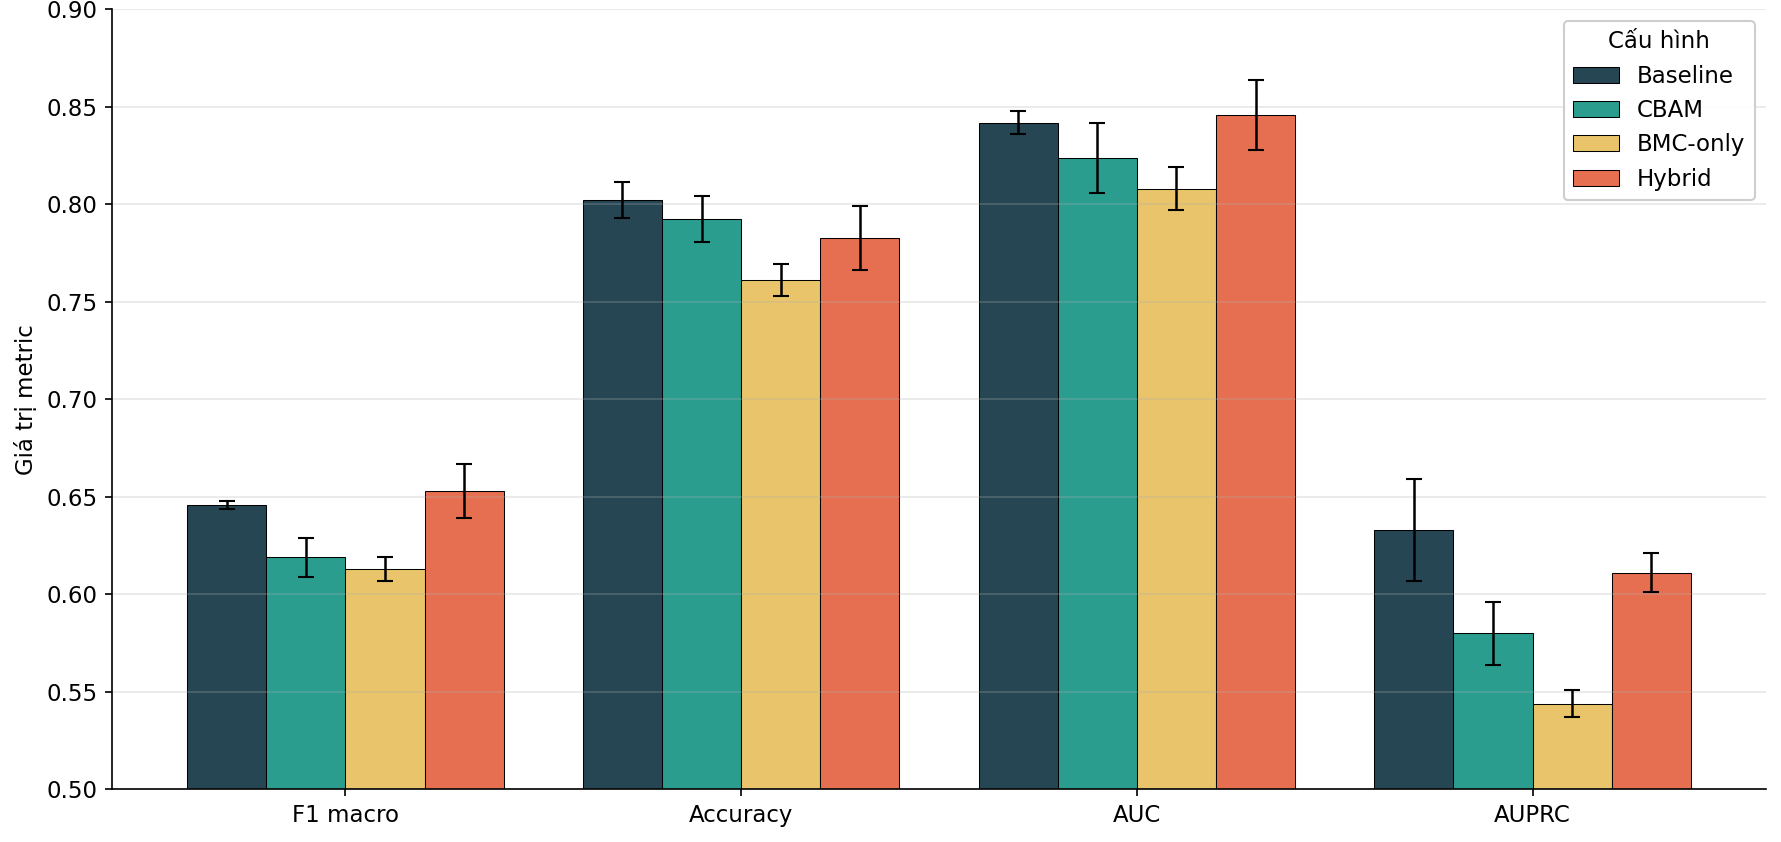
\includegraphics[width=0.95\textwidth]{cslt/spider_3seed_bars.png}
    \caption{SPIDER 8-label: 4 cấu hình $\times$ 4 metrics (3-seed).}
    \label{fig:spider_3seed_bars}
\end{figure}

% \textbf{Finding chính:} CBAM hoạt động \emph{ngược} trên SPIDER --- Mean F1 0.619 thấp hơn SpineNetV2 0.646 (chênh $-0.027$, vượt 2$\sigma$, có ý nghĩa thống kê) dù cải thiện rõ trên RSNA. Hybrid cân bằng tốt cross-dataset: ngang SpineNetV2 về F1 (0.653 vs 0.646, trong noise) nhưng không thoái hóa như CBAM-only. Lý giải: CBAM tinh chỉnh sâu cho phân bố RSNA dễ overfitting khi chuyển dataset; BiomedCLIP frozen trong Hybrid đóng vai trò \emph{regularizer} giúp giữ ổn định. AUPRC có trade-off (SpineNetV2 0.633 dẫn đầu, Hybrid 0.611) --- BiomedCLIP prior cải thiện ranking F1/AUC nhưng làm xáo trộn calibration của xác suất.

Bảng~\ref{tab:spider_per_disease} chi tiết theo từng nhóm bệnh với 6 chỉ số (Acc, Recall, Precision, F1, AUC, AUPRC) cho 3 cấu hình chính (SpineNetV2 / CBAM / Hybrid). Cách tiếp cận hybrid đạt giá trị tốt nhất ở phần lớn các chỉ số, chứng minh đặc trưng ngữ nghĩa của BiomedCLIP kết hợp với ngữ cảnh 3D của CBAM giúp tổng quát hóa tốt hơn trên dữ liệu mới.

\begin{table}[htbp]
\centering
\caption{Chi tiết SPIDER theo từng nhóm bệnh}
\label{tab:spider_per_disease}
\label{tab:spider_per_disease}
\renewcommand{\arraystretch}{1.15}
\setlength{\tabcolsep}{3pt}
\resizebox{\textwidth}{!}{%
\footnotesize
\begin{tabular}{llccccc}
\toprule
\textbf{Condition} & \textbf{Config} & \textbf{Recall} & \textbf{Precision} & \textbf{F1} & \textbf{AUC} & \textbf{AUPRC} \\
\midrule
\multirow{4}{*}{Modic (4-cls)}
 & SpineNetV2 & 0.374 $\pm$ 0.01 & 0.383 $\pm$ 0.02 & 0.376 $\pm$ 0.01 & 0.731 $\pm$ 0.03 & \textbf{0.545 $\pm$ 0.08} \\
 & CBAM     & 0.370 $\pm$ 0.01 & \textbf{0.385 $\pm$ 0.02} & 0.374 $\pm$ 0.01 & 0.807 $\pm$ 0.05 & 0.463 $\pm$ 0.05 \\
 & BMC-only & \textbf{0.389 $\pm$ 0.01} & 0.377 $\pm$ 0.02 & \textbf{0.381 $\pm$ 0.02} & 0.742 $\pm$ 0.05 & 0.474 $\pm$ 0.03 \\
 & Hybrid   & 0.382 $\pm$ 0.02 & 0.377 $\pm$ 0.01 & 0.379 $\pm$ 0.02 & \textbf{0.827 $\pm$ 0.04} & 0.500 $\pm$ 0.03 \\
\midrule
\multirow{4}{*}{Disc Narrowing}
 & SpineNetV2 & 0.820 $\pm$ 0.00 & \textbf{0.828 $\pm$ 0.01} & 0.823 $\pm$ 0.01 & \textbf{0.927 $\pm$ 0.01} & 0.882 $\pm$ 0.02 \\
 & CBAM     & 0.817 $\pm$ 0.02 & 0.819 $\pm$ 0.01 & 0.818 $\pm$ 0.01 & 0.896 $\pm$ 0.02 & 0.862 $\pm$ 0.01 \\
 & BMC-only & 0.802 $\pm$ 0.00 & 0.789 $\pm$ 0.01 & 0.792 $\pm$ 0.01 & 0.885 $\pm$ 0.01 & 0.829 $\pm$ 0.02 \\
 & Hybrid   & \textbf{0.836 $\pm$ 0.01} & 0.827 $\pm$ 0.01 & \textbf{0.831 $\pm$ 0.01} & 0.916 $\pm$ 0.02 & \textbf{0.884 $\pm$ 0.01} \\
\midrule
\multirow{4}{*}{Spondylolisthesis}
 & SpineNetV2 & 0.597 $\pm$ 0.05 & \textbf{0.793 $\pm$ 0.14} & \textbf{0.632 $\pm$ 0.05} & \textbf{0.826 $\pm$ 0.01} & \textbf{0.325 $\pm$ 0.11} \\
 & CBAM     & 0.500 $\pm$ 0.00 & 0.484 $\pm$ 0.00 & 0.492 $\pm$ 0.00 & 0.822 $\pm$ 0.03 & 0.251 $\pm$ 0.09 \\
 & BMC-only & 0.512 $\pm$ 0.03 & 0.497 $\pm$ 0.02 & 0.501 $\pm$ 0.02 & 0.775 $\pm$ 0.05 & 0.116 $\pm$ 0.04 \\
 & Hybrid   & \textbf{0.633 $\pm$ 0.05} & 0.607 $\pm$ 0.05 & 0.613 $\pm$ 0.04 & 0.815 $\pm$ 0.01 & 0.302 $\pm$ 0.05 \\
\midrule
\multirow{4}{*}{UP Endplate}
 & SpineNetV2 & 0.727 $\pm$ 0.02 & 0.746 $\pm$ 0.02 & 0.728 $\pm$ 0.03 & 0.820 $\pm$ 0.01 & \textbf{0.753 $\pm$ 0.01} \\
 & CBAM     & 0.725 $\pm$ 0.02 & 0.736 $\pm$ 0.02 & 0.729 $\pm$ 0.02 & 0.801 $\pm$ 0.02 & 0.693 $\pm$ 0.03 \\
 & BMC-only & 0.733 $\pm$ 0.01 & 0.724 $\pm$ 0.01 & 0.724 $\pm$ 0.01 & 0.795 $\pm$ 0.02 & 0.698 $\pm$ 0.02 \\
 & Hybrid   & \textbf{0.753 $\pm$ 0.02} & \textbf{0.748 $\pm$ 0.02} & \textbf{0.749 $\pm$ 0.02} & \textbf{0.828 $\pm$ 0.03} & 0.751 $\pm$ 0.03 \\
\midrule
\multirow{4}{*}{LOW Endplate}
 & SpineNetV2 & 0.754 $\pm$ 0.01 & \textbf{0.764 $\pm$ 0.01} & \textbf{0.757 $\pm$ 0.01} & 0.823 $\pm$ 0.02 & \textbf{0.775 $\pm$ 0.02} \\
 & CBAM     & \textbf{0.756 $\pm$ 0.02} & 0.757 $\pm$ 0.02 & 0.757 $\pm$ 0.02 & 0.808 $\pm$ 0.02 & 0.726 $\pm$ 0.03 \\
 & BMC-only & 0.715 $\pm$ 0.02 & 0.711 $\pm$ 0.02 & 0.712 $\pm$ 0.02 & 0.792 $\pm$ 0.02 & 0.709 $\pm$ 0.03 \\
 & Hybrid   & 0.743 $\pm$ 0.04 & 0.745 $\pm$ 0.04 & 0.744 $\pm$ 0.04 & \textbf{0.826 $\pm$ 0.03} & 0.763 $\pm$ 0.03 \\
\midrule
\multirow{4}{*}{Disc Herniation}
 & SpineNetV2 & 0.500 $\pm$ 0.00 & 0.470 $\pm$ 0.01 & 0.485 $\pm$ 0.00 & 0.852 $\pm$ 0.02 & \textbf{0.271 $\pm$ 0.05} \\
 & CBAM     & 0.500 $\pm$ 0.00 & 0.470 $\pm$ 0.01 & 0.485 $\pm$ 0.00 & 0.790 $\pm$ 0.03 & 0.246 $\pm$ 0.04 \\
 & BMC-only & 0.596 $\pm$ 0.07 & 0.556 $\pm$ 0.03 & 0.565 $\pm$ 0.04 & 0.799 $\pm$ 0.02 & 0.183 $\pm$ 0.05 \\
 & Hybrid   & \textbf{0.636 $\pm$ 0.04} & \textbf{0.592 $\pm$ 0.04} & \textbf{0.601 $\pm$ 0.04} & \textbf{0.860 $\pm$ 0.02} & 0.248 $\pm$ 0.10 \\
\midrule
\multirow{4}{*}{Disc Bulging}
 & SpineNetV2 & 0.778 $\pm$ 0.03 & 0.779 $\pm$ 0.03 & 0.777 $\pm$ 0.03 & \textbf{0.874 $\pm$ 0.02} & 0.840 $\pm$ 0.03 \\
 & CBAM     & 0.759 $\pm$ 0.01 & 0.764 $\pm$ 0.01 & 0.758 $\pm$ 0.01 & 0.840 $\pm$ 0.02 & 0.824 $\pm$ 0.03 \\
 
  & BMC-only  & 0.762 $\pm$ 0.01 & 0.768 $\pm$ 0.00 & 0.761 $\pm$ 0.01 & 0.851 $\pm$ 0.02 & 0.834 $\pm$ 0.03 \\
 & Hybrid  & \textbf{0.796 $\pm$ 0.01} & \textbf{0.794 $\pm$ 0.01} & \textbf{0.792 $\pm$ 0.01} & 0.873 $\pm$ 0.01 & \textbf{0.851 $\pm$ 0.03} \\
\bottomrule
\end{tabular}%
}
\end{table}

% \begin{table}[htbp]
% \centering
% \caption{Recall của các nhãn minority lâm sàng quan trọng}
% \label{tab:spider_minority_recall}
% \renewcommand{\arraystretch}{1.2}
% \setlength{\tabcolsep}{4pt}
% \resizebox{\textwidth}{!}{%
% \begin{tabular}{lccccc}
% \toprule
% \textbf{Condition} & \textbf{Prev. \%} & \textbf{SpineNetV2} & \textbf{CBAM} & \textbf{BMC-only} & \textbf{Hybrid} \\
% \midrule
% Modic Type 1 (rare)        & 0.3\% & 0.000 & 0.000 & 0.000 & 0.000 \\
% Modic Type 3 (rare)        & 0.5\% & 0.000 & 0.000 & 0.000 & 0.000 \\
% Disc Narrowing (Yes)       & 38\%  & 0.758 $\pm$ 0.03 & 0.770 $\pm$ 0.03 & 0.822 & \textbf{0.825 $\pm$ 0.02} \\
% \textbf{Spondylolisthesis Yes} & 3\%  & 0.200 $\pm$ 0.10 & 0.000 $\pm$ 0.00 & 0.056 & \textbf{0.300 $\pm$ 0.10} \\
% \textbf{Disc Herniation Yes}   & 5\%  & 0.000 $\pm$ 0.00 & 0.000 $\pm$ 0.00 & 0.270 & \textbf{0.356 $\pm$ 0.08} \\
% \bottomrule
% \end{tabular}%
% }
% \end{table}
Hybrid dẫn đầu về kết quả của các nhãn thiểu số có ý nghĩa lâm sàng (Disc Herniation, Disc Narrowing), nơi tận dụng được từ các data đã được pretraintd từ BiomedCLIP. Quan trọng hơn, Hybrid là cấu hình duy nhất dẫn đầu cả hai bộ dữ liệu (RSNA lẫn SPIDER khi chuyển tập). Nhánh
BiomedCLIP đóng vai trò chuẩn hóa, giúp mô hình không thoái hóa khi
chuyển sang dữ liệu khác (so với CBAM bị quá khớp với RSNA và thắng rất ít trên SPIDER). Đây là sự cân bằng cần thiết cho triển khai lâm sàng trên nhiều cơ sở y tế khác nhau.
\section{Thảo luận chung}


\textbf{Đóng góp về phương pháp.} Luận văn đã đề xuất kiến trúc Hybrid. Đây là một trong các báo cáo đầu tiên trên cùng dataset có 3-seed mean$\pm$std cho cross-dataset transfer learning.

\textbf{Hạn chế và hướng tiếp theo.} Hướng phát triển sâu hơn được trình bày trong Chương 7.

\clearpage

\chapter{PHẦN MỀM HỖ TRỢ BÁC SĨ GÁN NHÃN}
\label{chap:software}

\section{Mục tiêu và yêu cầu}
\label{sec:sw_requirements}

Phần mềm được xây dựng nhằm hỗ trợ bác sĩ trong quá trình đọc phim MRI cột sống thắt lưng, với mục tiêu rút ngắn thời gian đọc phim chứ không thay thế vai trò chẩn đoán của bác sĩ. Từ mục tiêu đó, ba yêu cầu sau được đặt ra:

\begin{itemize}
    \item \textbf{Trực quan hóa kết quả trên ảnh:} Kết quả phân vùng phải được tô màu trực tiếp trên ảnh MRI, kèm chú giải từng cấu trúc giải phẫu, để bác sĩ đối chiếu được bằng mắt thay vì chỉ đọc một bảng điểm tách rời khỏi ảnh.
    \item \textbf{Cho phép chỉnh sửa toàn bộ nhãn:} Mọi nhãn do mô hình sinh ra đều phải chỉnh sửa được, vì bác sĩ là người đưa ra kết luận cuối cùng.
    \item \textbf{Lưu lại các chỉnh sửa của bác sĩ:} Mỗi lần bác sĩ sửa một nhãn, hệ thống phải ghi lại cả giá trị mô hình dự đoán lẫn giá trị bác sĩ chỉnh, kèm thông tin ca chụp và tầng đĩa đệm, để dữ liệu này dùng được cho các nghiên cứu tiếp theo.
\end{itemize}

\section{Kiến trúc hệ thống}
\label{sec:sw_architecture}

\subsection{Tổng quan các thành phần}

Hệ thống chia làm hai phần chạy độc lập. Phần máy chủ viết bằng FastAPI, giữ cơ sở dữ liệu và gọi hai mô hình: TotalSpineSeg để phân vùng và mô-đun grading Hybrid để chấm nhãn. Ảnh MRI và mặt nạ phân vùng lưu trên ổ đĩa, còn thông tin ca chụp và nhãn lưu trong cơ sở dữ liệu. Phần giao diện viết bằng React kết hợp thư viện Cornerstone3D, vốn là thư viện chuyên dùng để hiển thị ảnh y tế trên trình duyệt.

TotalSpineSeg được cài trong một môi trường Python riêng và gọi qua dòng lệnh, không nhập trực tiếp vào mã nguồn máy chủ. Lý do là hai mô hình đòi hỏi những phiên bản thư viện khác nhau; tách môi trường thì nâng cấp mô hình này không làm hỏng mô hình kia. Hình~\ref{fig:sw_architecture} mô tả các thành phần và quan hệ giữa chúng.

\begin{figure}[htbp]
    \centering
    \begin{tikzpicture}[
        comp/.style={rectangle, draw=blue, fill=blue!8, rounded corners, minimum width=3.3cm,
                     minimum height=1.0cm, align=center, thick, font=\small},
        store/.style={rectangle, draw=green!50!black, fill=green!10, rounded corners,
                      minimum width=3.3cm, minimum height=1.0cm, align=center, thick, font=\small},
        model/.style={rectangle, draw=orange!80!black, fill=orange!10, rounded corners,
                      minimum width=3.3cm, minimum height=1.0cm, align=center, thick, font=\small},
        ar/.style={->, thick, blue!70!black}
    ]
        \node[comp]  (fe)   at (0,3.3)     {\textbf{Giao diện}\\\scriptsize React + Cornerstone3D};
        \node[comp]  (be)   at (0,1.2)     {\textbf{Máy chủ}\\\scriptsize FastAPI};
        \node[model] (seg)  at (-4.3,-1.1) {\textbf{Phân vùng}\\\scriptsize TotalSpineSeg};
        \node[model] (grd)  at (0,-1.1)    {\textbf{Chấm nhãn}\\\scriptsize Hybrid};
        \node[store] (db)   at (4.8,1.2)   {\textbf{Cơ sở dữ liệu}\\\scriptsize ca chụp, nhãn,\\\scriptsize nhật ký hiệu chỉnh};
        \node[store] (fs)   at (4.8,-1.1)  {\textbf{Ổ đĩa}\\\scriptsize ảnh MRI, mặt nạ};

        \draw[ar] (fe) -- node[right,font=\scriptsize]{HTTP} (be);
        \draw[ar] (be) -- (seg);
        \draw[ar] (be) -- (grd);
        \draw[ar] (be) -- (db);
        \draw[ar] (be) -- (fs);
        \draw[ar] (seg) -- (grd);
    \end{tikzpicture}
    \caption{Các thành phần của phần mềm.}
    \label{fig:sw_architecture}
\end{figure}

\subsection{Luồng xử lý một ca chụp}

Một ca đi qua năm bước. Bác sĩ tải lên một thư mục DICOM đã nén; máy chủ giải nén, nhận diện các chuỗi ảnh và dựng khối ba chiều. Tiếp theo TotalSpineSeg phân vùng, cho ra mặt nạ các đốt sống và đĩa đệm. Từ mặt nạ này hệ thống định vị từng đĩa đệm rồi cắt khối ảnh quanh nó, đưa qua mô-đun grading để chấm nhãn. Kết quả hiện lên giao diện cho bác sĩ xem và sửa. Cuối cùng, những ô bác sĩ sửa được ghi vào nhật ký hiệu chỉnh.

\section{Các chức năng chính}
\label{sec:sw_features}

\subsection{Quản lý ca chụp}

Màn hình đầu tiên là danh sách ca, nhóm theo bệnh nhân (Hình~\ref{fig:app_caselist}). Mỗi bác sĩ có một phòng riêng, đăng nhập bằng mã PIN bốn số, và chỉ thấy ca trong phòng của mình. Cách chia này để nhiều bác sĩ cùng thử phần mềm mà không nhìn thấy kết quả của nhau, nhờ đó nhận xét của họ độc lập với nhau.

\begin{figure}[htbp]
    \centering
    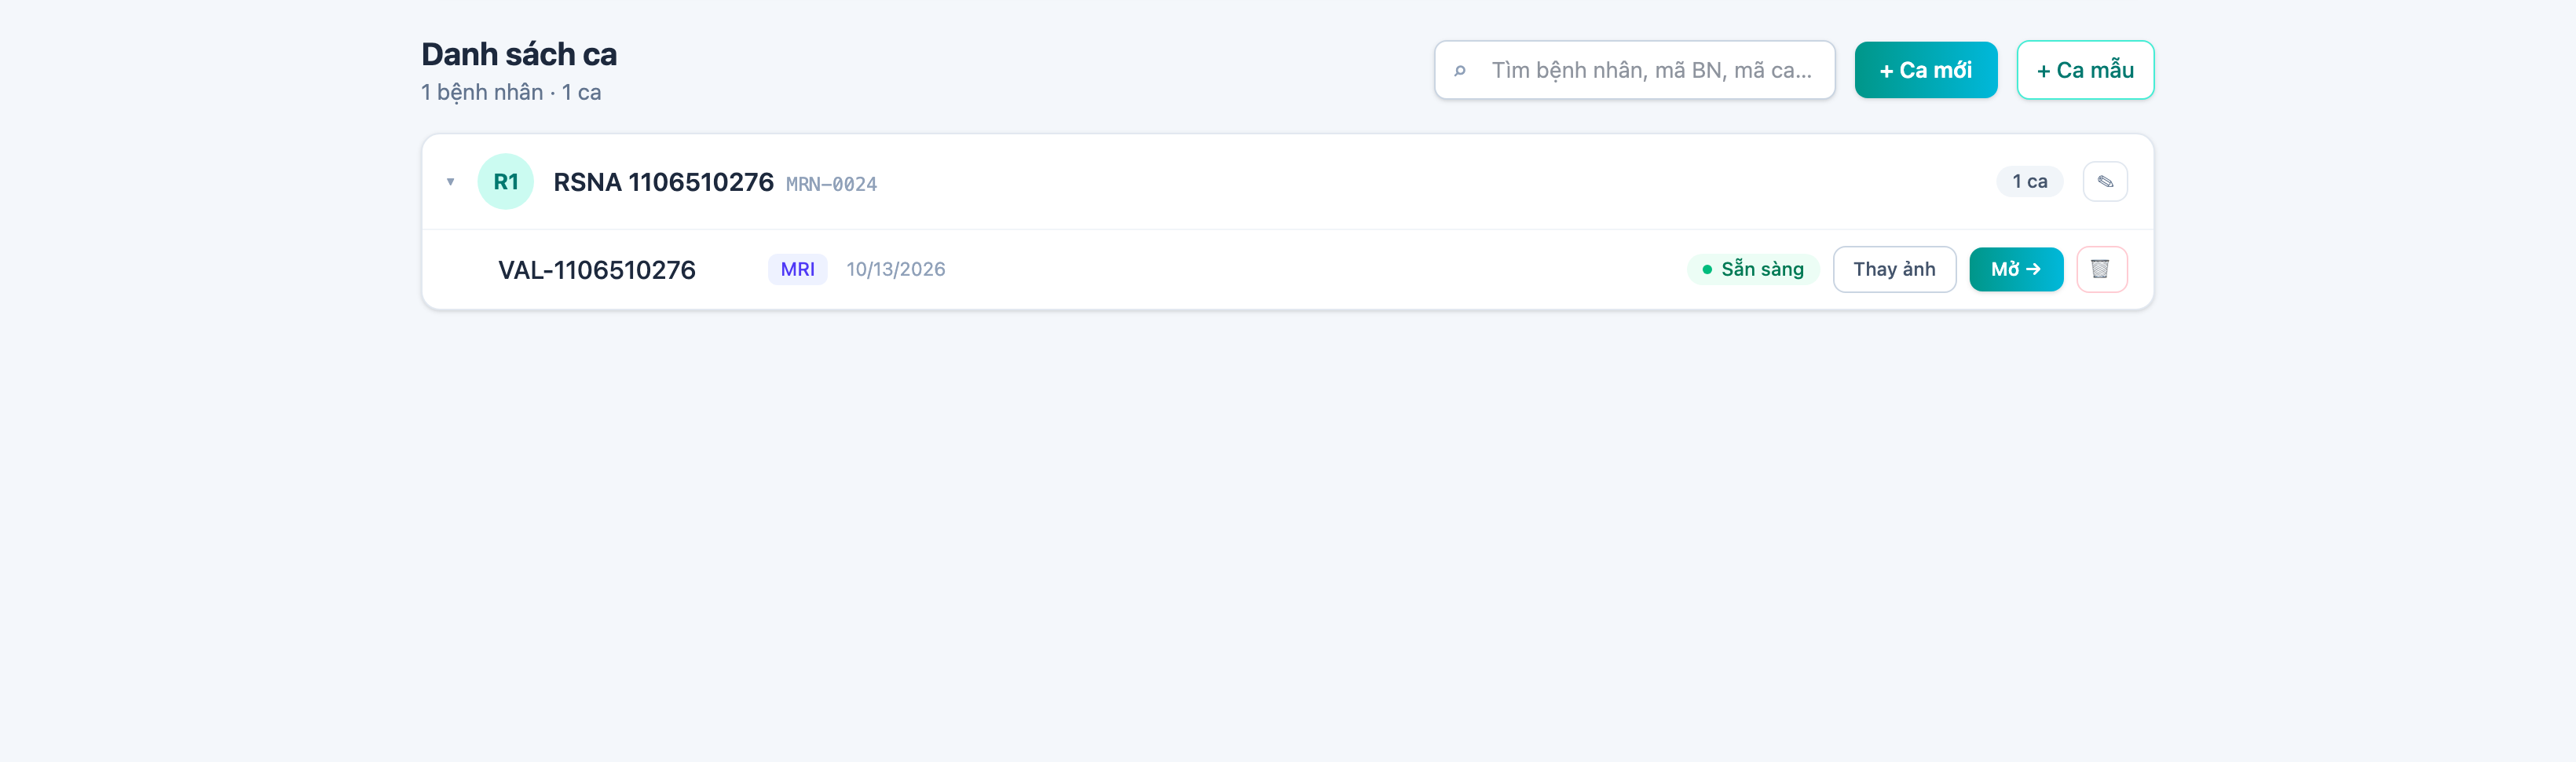
\includegraphics[width=\textwidth]{cslt/app_caselist.png}
    \caption{Màn hình danh sách ca chụp.}
    \label{fig:app_caselist}
\end{figure}

Bác sĩ có thể tạo ca mới rồi tải phim của mình lên, hoặc thêm một ca mẫu đã được chấm sẵn để thử nhanh. Ca mẫu là bản sao riêng của từng phòng, nên bác sĩ sửa thoải mái mà không ảnh hưởng người khác.

\subsection{Xem ảnh và kết quả phân vùng}

Màn hình đọc phim là nơi bác sĩ làm việc nhiều nhất (Hình~\ref{fig:app_viewer}). Ảnh MRI hiển thị ở giữa, mặt nạ phân vùng tô màu chồng lên, mỗi cấu trúc một màu và có chú giải bên phải. Bác sĩ chỉnh được độ trong của lớp màu, tắt hẳn lớp màu để nhìn ảnh gốc, chuyển lát cắt bằng con lăn chuột, và chỉnh độ sáng, độ tương phản bằng cách kéo chuột. Với máy không có chuột, mọi thao tác trên đều có nút bấm tương ứng ở dưới ảnh.

\begin{figure}[htbp]
    \centering
    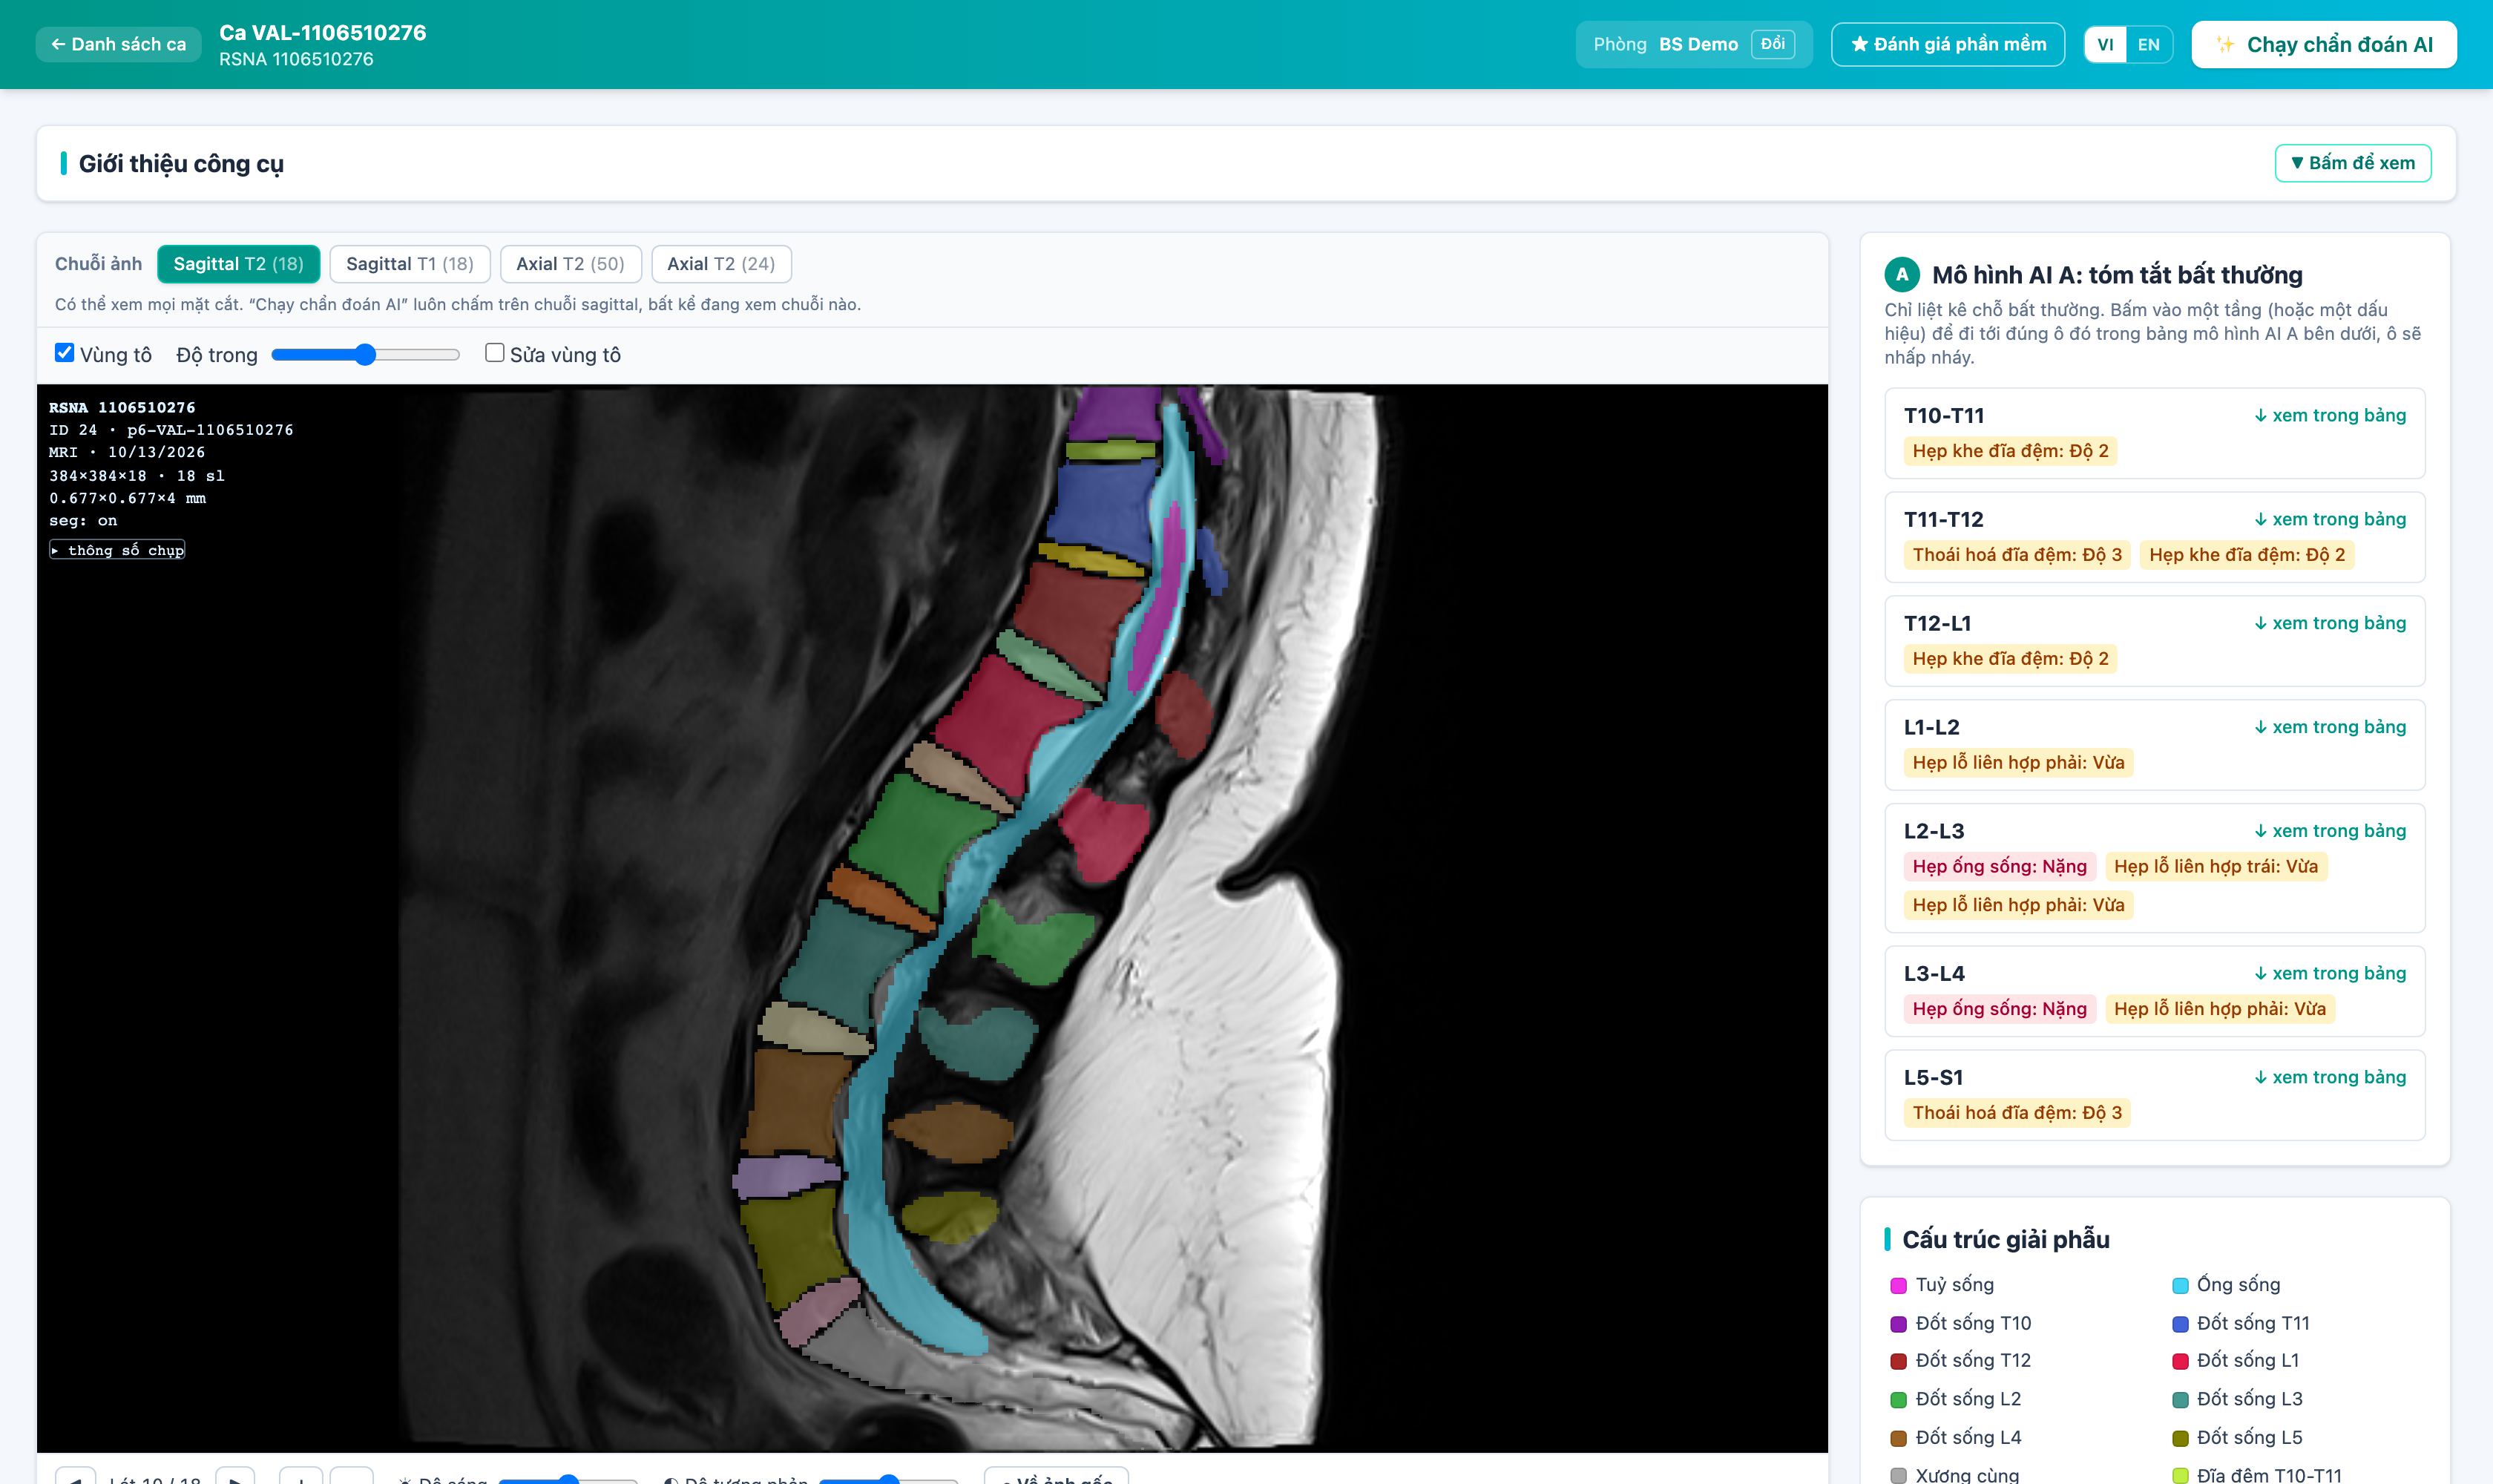
\includegraphics[width=\textwidth]{cslt/app_viewer.png}
    \caption{Màn hình đọc phim.}
    \label{fig:app_viewer}
\end{figure}

Bên phải ảnh là khung tóm tắt, chỉ liệt kê những tầng đĩa đệm có dấu hiệu bất thường kèm mức độ. Bác sĩ bấm vào một dòng thì giao diện cuộn xuống đúng ô tương ứng trong bảng nhãn và làm ô đó nhấp nháy. Mục đích là để bác sĩ không phải dò cả bảng mười một dòng khi chỉ muốn kiểm tra một chỗ.

\subsection{Xem và chỉnh sửa nhãn}

Kết quả chấm nhãn trình bày dưới dạng bảng mười một nhãn bệnh lý theo tám tầng đĩa đệm, từ T10--T11 đến L5--S1 (Hình~\ref{fig:app_grading_table}). Mỗi ô là một hộp chọn: bác sĩ bấm vào là đổi được giá trị. Ô được tô màu theo mức độ, đỏ cho mức nặng và vàng cho mức vừa, để chỗ cần chú ý nổi lên ngay. Những ô mà mô hình ít chắc chắn có thêm một dấu cảnh báo.

\begin{figure}[htbp]
    \centering
    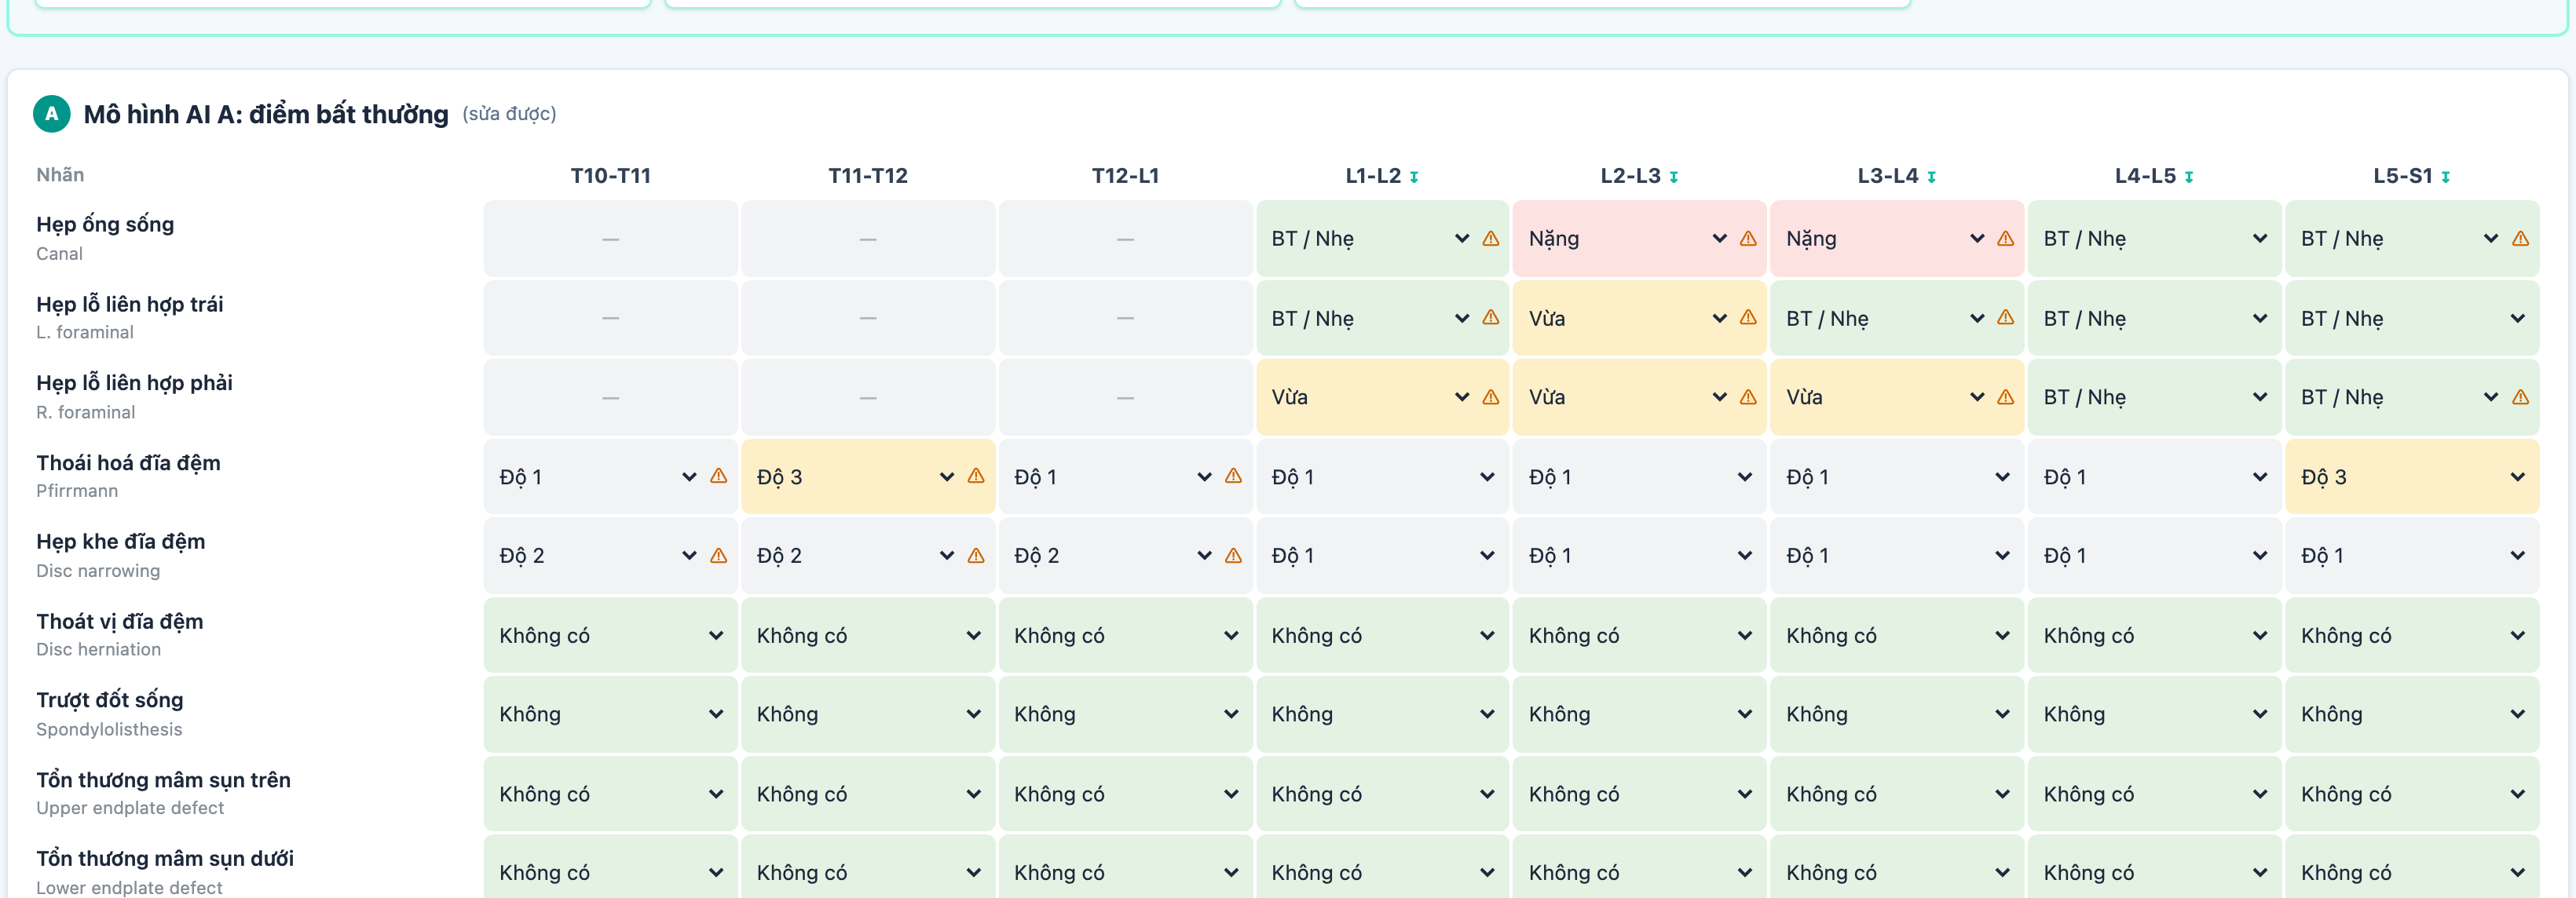
\includegraphics[width=\textwidth]{cslt/app_grading_table.png}
    \caption{Bảng chấm nhãn theo tầng đĩa đệm.}
    \label{fig:app_grading_table}
\end{figure}

Ba nhãn hẹp ống sống và hẹp lỗ liên hợp trái, phải để trống ở các tầng ngực trên, vì bộ dữ liệu huấn luyện chỉ gán nhãn từ tầng L1--L2 trở xuống; để trống thay vì đưa ra một giá trị không có cơ sở.

Dưới bảng còn ô ghi kết luận của bác sĩ bằng chữ. Phần này không bắt buộc, nhưng để bác sĩ ghi thêm những gì bảng điểm không thể hiện được.

\subsection{Ghi nhận chỉnh sửa của bác sĩ}

Mỗi lần bác sĩ sửa một ô trong bảng nhãn rồi bấm lưu, hệ thống ghi lại cặp giá trị mô hình dự đoán và giá trị bác sĩ chỉnh, kèm mã ca chụp và tầng đĩa đệm tương ứng. Các bản ghi này được gom thành từng lô (Hình~\ref{fig:app_corrections}).

\begin{figure}[htbp]
    \centering
    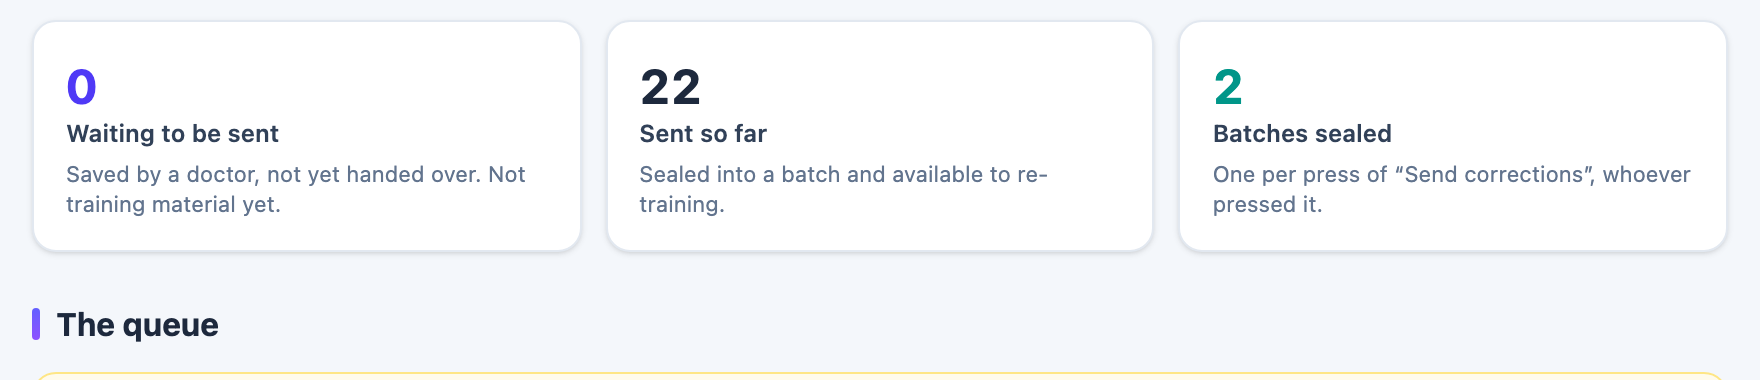
\includegraphics[width=0.9\textwidth]{cslt/app_corrections.png}
    \caption{Thống kê chỉnh sửa của bác sĩ.}
    \label{fig:app_corrections}
\end{figure}

Các chỉnh sửa được gom chung cho cả hệ thống chứ không theo từng ca, vì một ca chỉ có vài đĩa đệm, quá ít để huấn luyện. Trong đợt thử nghiệm, hệ thống đã ghi nhận 22 chỉnh sửa và gom thành hai lô.

Hiện tại phần mềm mới chỉ dừng ở việc lưu lại các chỉnh sửa. Mô hình chưa học lại được từ những dữ liệu này; phần huấn luyện lại được đặt làm hướng phát triển ở Chương 7.

\section{Nhận xét từ bác sĩ}
\label{sec:sw_doctor_feedback}

% ===================================================================
% MỤC NÀY ĐỂ TRỐNG CÓ CHỦ Ý cho lần nộp theo hạn.
% GVHD (TS. Phan Trọng Nhân, tin nhắn ngày 13/10/2026):
%   "Em cứ nộp theo hạn, phần BS nhận xét sẽ bổ sung khi gặp phản biện
%    và khi báo cáo HĐ."
%   "Vẫn viết vào báo cáo cuối cùng nộp cho khoa nha -- vì ở HĐ em show
%    ra có được tính điểm, nên báo cáo cuối cùng vẫn phải có nha."
% => BẮT BUỘC điền trước khi nộp bản cuối cho khoa.
% ===================================================================

Phần mềm có sẵn phiếu đánh giá để bác sĩ trả lời sau khi đọc vài ca. Kết quả thu thập từ bác sĩ sẽ được bổ sung vào mục này.

\clearpage

\chapter{KẾT LUẬN VÀ HƯỚNG PHÁT TRIỂN}

\section{Tổng kết}

Luận văn đã xây dựng một giải pháp hỗ trợ bác sĩ gán nhãn ảnh MRI cột sống thắt lưng, gồm hai phần gắn với nhau: một mô hình đánh giá mức độ thoái hóa cho từng đĩa đệm, và một phần mềm đưa mô hình đó tới tay người dùng. Các kết quả chính được tóm tắt dưới đây.

\textbf{Lựa chọn mô-đun phân vùng.} TotalSpineSeg được chọn sau khi so sánh với ba mô hình khác là SPINEPS, MedCLIP-SAMv2 và SpineNetV2. Mô hình đạt độ chính xác dương tính 97.87\%, vượt xa SPINEPS (52.17\%), MedCLIP-SAMv2 (29.16\%) và SpineNetV2 (51.76\%), nên vùng trích xuất gần như không nhiễu. Chỉ số Recall thấp hơn (56.49\%) đến từ khác biệt về định nghĩa nhãn, do TotalSpineSeg chỉ phân vùng thân đốt sống mà không tính gai sau; bù lại, sai số bề mặt thấp nhất trong nhóm (ASSD 6.85 mm) khiến đây là lựa chọn phù hợp để định vị vùng quan tâm.

\textbf{Lựa chọn mô-đun đánh giá bất thường.} SpineNetV2 được chọn làm kiến trúc nền. Trên ba nhóm bệnh lý chính, mô hình đạt F1 trung bình 77.50\%, thấp hơn Ning Shen khoảng ba điểm nhưng được ưu tiên nhờ mã nguồn mở và kiến trúc đủ đơn giản để tinh chỉnh sâu, trong khi Ning Shen là tổ hợp nhiều mô hình lớn, khó duy trì. MedGemma bị loại vì Recall chỉ 6--21\% trên bệnh lý cột sống thắt lưng do chưa được chuyên biệt hóa.

\textbf{Đóng góp chính về mô hình.} Luận văn đề xuất kiến trúc Hybrid hai nhánh, kết hợp một nhánh chú ý CBAM trên ResNet-34 ba chiều với một nhánh BiomedCLIP được giữ đông cứng, cùng một quy trình xử lý mất cân bằng lớp. Trên RSNA 2024, so với SpineNetV2, kiến trúc này nâng Mean F1 macro từ 0.420 lên 0.527 và Mean Recall từ 0.412 lên 0.592. Cải thiện rõ nhất nằm ở lớp Severe: Severe Recall tăng từ 12.3\% lên 48.6\%, gấp khoảng bốn lần, còn Severe F1 tăng từ 0.152 lên 0.356. Cái giá là Mean Accuracy giảm 8.6 điểm, do mô hình nền đạt độ chính xác cao chủ yếu nhờ dự đoán thiên về lớp đa số. Trong bối cảnh lâm sàng, bỏ sót một ca nặng nghiêm trọng hơn một lần báo động nhầm, nên đây là đánh đổi có chủ ý.

\textbf{Mở rộng không gian nhãn.} Vì dự đoán được thực hiện bằng cách so khớp với câu mô tả nhãn, tập nhãn trở thành đầu vào của suy luận. Trên bộ dữ liệu SPIDER đến từ bệnh viện khác và dùng lược đồ nhãn khác, mô hình chấm được tám nhãn chưa từng thấy mà không huấn luyện lại dòng nào, đạt F1 trung bình 0.362. Khi cho phép huấn luyện có giám sát, mô hình đạt 0.653 so với 0.646 của SpineNetV2, tức ngang bằng, trong khi cấu hình chỉ dùng CBAM tụt xuống 0.619. Điều này cho thấy nhánh đông cứng giữ cho lợi thế của cơ chế chú ý không mất đi khi đổi bộ dữ liệu.

\textbf{Phần mềm hỗ trợ bác sĩ.} Luận văn hiện thực một phần mềm cho phép tải ảnh DICOM, phân vùng tự động, chấm mười một nhãn bệnh lý theo từng tầng đĩa đệm, hiển thị kết quả trực tiếp trên ảnh, và cho bác sĩ chỉnh sửa mọi nhãn. Mọi chỉnh sửa đều được lưu lại làm dữ liệu. Phần máy chủ có 209 bài kiểm thử tự động.

\textbf{Kết quả đã được công bố.} Một phần kết quả của luận văn, cụ thể là kiến trúc Hybrid hai nhánh và cơ chế mở rộng không gian nhãn zero-shot, đã được chấp nhận và trình bày tại hội nghị quốc tế MIWAI 2026 (\textit{The 18th Multi-disciplinary International Conference on Artificial Intelligence}), tổ chức tại Halifax, Nova Scotia, Canada, ngày 10--12/10/2026. Bài báo có nhan đề \textit{``A Two-Branch Hybrid Model for Imbalanced Lumbar Disc Grading and Zero-Shot Label Extension''}, học viên là tác giả thứ nhất và TS. Phan Trọng Nhân là tác giả liên hệ, được xuất bản trong bộ \textit{Lecture Notes in Artificial Intelligence} của Springer. Việc bài báo vượt qua vòng phản biện quốc tế là một kiểm chứng độc lập cho phương pháp đề xuất.

\section{Hạn chế}

Luận văn còn một số hạn chế cần nêu rõ.

\textbf{Mức độ phát hiện ca nặng chưa đủ cho sàng lọc độc lập.} Severe Recall 48.6\% tuy gấp bốn lần mô hình nền nhưng vẫn thấp hơn nhiều so với mức khoảng 80\% mà một công cụ sàng lọc cần đạt. Vì vậy hệ thống chỉ nên dùng như người đọc thứ hai, đánh dấu những ca nghi ngờ để bác sĩ xem lại, chứ chưa thể dùng độc lập.

\textbf{Kết quả yếu hơn ở hai nhóm lỗ liên hợp.} Severe Recall ở hai điều kiện này chỉ nằm trong khoảng 18--22\%, thấp hơn hẳn so với ống sống. Các nghiên cứu kiểm chứng độc lập trên SpineNetV2 cũng ghi nhận giới hạn tương tự khi chỉ đọc mặt cắt dọc, nên nhiều khả năng đây là giới hạn của dữ liệu đầu vào chứ không phải của kiến trúc.

\textbf{Số lần chạy còn ít.} Mọi kết quả lấy trung bình qua ba hạt giống ngẫu nhiên. Đây là mức đủ để thấy xu hướng nhưng chưa đủ để kết luận có ý nghĩa thống kê chặt chẽ.

\textbf{Chưa đánh giá trên dữ liệu bệnh viện trong nước.} Hai bộ dữ liệu sử dụng đều là dữ liệu công khai của nước ngoài. Hiệu năng trên ảnh chụp tại các cơ sở y tế Việt Nam, với máy chụp và thông số khác, chưa được kiểm chứng.

\section{Hướng phát triển}

\subsection{Cơ chế học lại từ phản hồi của bác sĩ}

Phần mềm hiện đã thu thập và lưu trữ mọi chỉnh sửa của bác sĩ, nhưng chưa có cơ chế để mô hình học lại từ những dữ liệu đó. Đây là hướng phát triển trực tiếp nhất.

Một vòng phản hồi hoàn chỉnh cần ba phần còn thiếu. Thứ nhất là quy trình huấn luyện lại từ một lô chỉnh sửa, với bài toán khó là số mẫu mỗi lô rất ít so với tập huấn luyện gốc, nên cần kỹ thuật tránh việc mô hình quên những gì đã học. Thứ hai là cách đánh giá phiên bản mới một cách đáng tin trước khi đưa vào dùng. Thứ ba là bước người duyệt: nếu để mô hình tự cập nhật, chỉ vài chỉnh sửa sai cũng đủ làm chất lượng đi xuống mà không ai phát hiện, nên quyết định đưa phiên bản mới vào sử dụng vẫn nên thuộc về con người.

\subsection{Bổ sung mặt cắt ngang cho hai nhóm lỗ liên hợp}

Như đã nêu ở phần hạn chế, hai điều kiện hẹp lỗ liên hợp bị giới hạn bởi thông tin mà mặt cắt dọc cung cấp. Hướng khắc phục là đưa thêm mặt cắt ngang vào mô hình, đồng thời tinh chỉnh TotalSpineSeg để phân vùng chính xác trên mặt cắt này. Có mặt nạ đúng trên cả hai mặt phẳng sẽ giúp định vị vùng tổn thương chính xác hơn, từ đó nâng chất lượng chấm nhãn.

\subsection{Kiến trúc thị giác ngôn ngữ ba chiều}

Nhánh đa phương thức hiện dùng BiomedCLIP, vốn là mô hình hai chiều: nó đọc từng lát một rồi mới gộp lại, nên không nắm được quan hệ không gian giữa các lát. Một mô hình thị giác ngôn ngữ huấn luyện sẵn trên dữ liệu y khoa ba chiều sẽ là nền tốt hơn cho nhánh này.

\subsection{Sinh báo cáo chẩn đoán bằng ngôn ngữ tự nhiên}

Hệ thống hiện trả về nhãn và mức độ. Một bước mở rộng là sinh ra đoạn mô tả bằng lời để bác sĩ tham khảo khi viết kết luận. Khảo sát ở Chương 5 cho thấy MedGemma nguyên bản có Recall rất thấp trên bệnh lý thắt lưng nên không đưa được vào hệ thống, nhưng việc tinh chỉnh một mô hình như vậy trên các cặp ảnh và văn bản chẩn đoán của chính lĩnh vực này là hướng đáng thử.

\subsection{Đánh giá cùng bác sĩ trên dữ liệu thực tế}

Cuối cùng, hệ thống cần được đánh giá bởi chính người sẽ dùng nó. Phần mềm đã có sẵn phiếu đánh giá và cơ chế ghi nhận chỉnh sửa, nên việc còn lại là tổ chức một đợt sử dụng thực tế với bác sĩ chuyên khoa trên dữ liệu của bệnh viện trong nước, vừa để đo mức độ hữu ích, vừa để thu thập dữ liệu cho vòng phản hồi nói trên.

% \clearpage

\renewcommand{\bibname}{Tài liệu tham khảo}
\bibliographystyle{ieeetr}
% Tránh LaTeX tự ngắt từ tiếng Anh bằng gạch nối trong danh mục tham khảo
% (vd: "trans-formers", "seg-mentation"); ưu tiên giãn khoảng cách hơn.
\begingroup
\hyphenpenalty=10000
\exhyphenpenalty=10000
\sloppy
\bibliography{thesiscite}
\endgroup

\appendix
% \chapter{Phân công nhiệm vụ}
% \section{Nhận xét quá trình làm việc}
% Trong quá trình làm việc, các thành viên trong nhóm đã tích cực nghiên cứu, hoàn thành công việc theo đúng tiến độ đề ra. Nhóm cũng thực hiện báo cáo tiến độ cho giảng viên hướng dẫn theo lịch trình một cách đầy đủ và chi tiết để nhận được những nhận xét, góp ý kịp thời.

% Về mặt phân công, trong suốt quá trình làm việc, các thành viên đều có sự tham gia ít nhiều đối với tất cả các phần của Đồ án. Điều này giúp các thành viên hiểu và nắm rõ toàn bộ nội dung của đồ án, cũng như có thể trực tiếp tham gia hỗ trợ lẫn nhau và dễ dàng hơn trong việc phối hợp. Bên cạnh đó, để có để đạt được hiệu quả tốt nhất thì việc phân công vẫn dựa trên điểm mạnh và điểm yếu của từng thành thành viên, nhưng vẫn đảm bảo tính hợp lý về mặt thời gian và công bằng về khối lượng công việc.
% \section{Chi tiết phân công nhiệm vụ}
% Chi tiết phân công nhiên vụ cho từng thành viên được thể hiện trong bảng \ref{tab:phan_cong}.

% \begin{table}[!htp]
%     \centering
%     \caption{Bảng chi tiết phân công nhiệm vụ}
%     \begin{tabular}{|c|c|}
%     \hline
%         \textbf{Thành viên} & \textbf{Phân công nhiệm vụ}\\
%         \hline
%         \textbf{Hà Trung Kiên} & \makecell[l]{
%         Nghiên cứu các công trình liên quan.\\
%         Nghiên cứu các kiến thức nền tảng.\\
%         Phân tích và thiết kế các yêu cầu hệ thống.\\
%         Hiện thực các microservice về User, Project,...\\
%         Nghiên cứu các phương án cần thiết. \\
%         Triển khai hệ thống.
%         \\
%         }\\
%         \hline
%         \textbf{Lương Hồng Tiến Đạt} &  \makecell[l]{Nghiên cứu các kiến thức nền tảng.\\Nghiên cứu các công trình liên quan.\\Phân tích và thiết kế các yêu cầu hệ thống.\\ Thiết kế Database và kiến trúc hệ thống. \\ Hiện thực các microservice về Suggestion, Forum,... \\
%         Triển khai hệ thống.
%         \\}\\
%         \hline
%         \textbf{Hà Phan Thiên Phú} &  \makecell[l]{Nghiên cứu các kiến thức nền tảng.\\Nghiên cứu các công trình liên quan.\\
%          Phân tích và thiết kế các yêu cầu hệ thống.\\
%          Thiết kế giao diện cho hệ thống.\\
%         Hiện thực phần frontend cho hệ thống.\\
%         Triển khai hệ thống.
%          }\\
%         \hline
%     \end{tabular}
%     \label{tab:phan_cong}
% \end{table}
\end{document}



